\documentclass[a4paper]{article}
\usepackage[spanish]{babel}
\usepackage[utf8]{inputenc}
\usepackage{fancyhdr}
\usepackage{charter} % tipografia
%\usepackage{graphicx}
\usepackage[pdftex]{graphicx}
\usepackage{sidecap}
\usepackage{caption}
\usepackage{subcaption}
\usepackage{booktabs}
\usepackage{makeidx}
\usepackage{float}
\usepackage{amsmath, amsthm, amssymb}
\usepackage{amsfonts}
\usepackage{sectsty}
\usepackage{charter}
\usepackage{wrapfig}
\usepackage{listings}
\usepackage{hyperref} % links
\usepackage{algorithm} %http://www.ctan.org/pkg/algorithms
\usepackage{algorithmic}
\usepackage{color} % para snipets de codigo coloreados
\usepackage{fancybox} % para el sbox de los snipets de codigo
\definecolor{litegrey}{gray}{0.94}
% \newenvironment{sidebar}{%
% \begin{Sbox}\begin{minipage}{.85\textwidth}}%
% {\end{minipage}\end{Sbox}%
% \begin{center}\setlength{\fboxsep}{6pt}%
% \shadowbox{\TheSbox}\end{center}}
% \newenvironment{warning}{%
% \begin{Sbox}\begin{minipage}{.85\textwidth}\sffamily\lite\small\RaggedRight}%
% {\end{minipage}\end{Sbox}%
% \begin{center}\setlength{\fboxsep}{6pt}%
% \colorbox{litegrey}{\TheSbox}\end{center}}

%\newenvironment{codesnippet}{%
%\begin{Sbox}\begin{minipage}{\linewidth-2\fboxsep-2\fboxrule-4pt}\sffamily\small}%
%{\end{minipage}\end{Sbox}%
%\begin{center}%
%\colorbox{litegrey}{\TheSbox}\end{center}}

% \newenvironment{codesnippet}{\VerbatimEnvironment%
%   \noindent
%   %{\columnwidth-\leftmargin-\rightmargin-2\fboxsep-2\fboxrule-4pt}
%   \begin{Sbox}
%   \begin{minipage}{\linewidth-2\fboxsep-2\fboxrule-4pt}
%   \begin{Verbatim}
% }{%
%   \end{Verbatim}
%   \end{minipage}
%   \end{Sbox}%
%   \colorbox{litegrey}{\TheSbox}
% }

\newenvironment{codesnippet}{\VerbatimEnvironment%
  \noindent
  %      {\columnwidth-\leftmargin-\rightmargin-2\fboxsep-2\fboxrule-4pt}
  \begin{Sbox}
  \begin{minipage}{\linewidth}
  \begin{Verbatim}
}{%
  \end{Verbatim}
  \end{minipage}
  \end{Sbox}%
  \colorbox{litegrey}{\TheSbox}
}
\usepackage{fancyhdr}
\pagestyle{fancy}
%\renewcommand{\chaptermark}[1]{\markboth{#1}{}}
\renewcommand{\sectionmark}[1]{\markright{\thesection\ - #1}}
\fancyhf{}
\fancyhead[LO]{Sección \rightmark} % \thesection\
\fancyfoot[LO]{\small{Iv\'an Arcuschin, Mart\'in Jedwabny, Jos\'e Massigoge, Lucas Puterman}}
\fancyfoot[RO]{\thepage}
\renewcommand{\headrulewidth}{0.5pt}
\renewcommand{\footrulewidth}{0.5pt}
\setlength{\hoffset}{-0.8in}
\setlength{\textwidth}{16cm}
%\setlength{\hoffset}{-1.1cm}
%\setlength{\textwidth}{16cm}
\setlength{\headsep}{0.5cm}
\setlength{\textheight}{25cm}
\setlength{\voffset}{-0.7in}
\setlength{\headwidth}{\textwidth}
\setlength{\headheight}{13.1pt}
\renewcommand{\baselinestretch}{1.1} % line spacing
% \setcounter{secnumdepth}{2}
\usepackage{underscore}
\usepackage{caratula}
\usepackage{url}
\usepackage[usenames,dvipsnames]{xcolor}
\lstset{
    language=C++,
    basicstyle=\ttfamily,
    keywordstyle=\color{blue}\ttfamily,
    stringstyle=\color{red}\ttfamily,
    commentstyle=\color{ForestGreen}\ttfamily,
    morecomment=[l][\color{magenta}]{\#}
}
% ******************************************************** %
% TEMPLATE DE INFORME ORGA2 v0.1 %
% ******************************************************** %
% ******************************************************** %
% %
% ALGUNOS PAQUETES REQUERIDOS (EN UBUNTU): %
% ========================================
% %
% texlive-latex-base %
% texlive-latex-recommended %
% texlive-fonts-recommended %
% texlive-latex-extra? %
% texlive-lang-spanish (en ubuntu 13.10) %
% ******************************************************** %
\begin{document}
\thispagestyle{empty}
\materia{Algoritmos y Estructura de Datos III}
\submateria{Primer Cuatrimestre de 2015}
\titulo{Trabajo Práctico I}
%\subtitulo{Grupo: }
\integrante{Iv\'an Arcuschin}{678/13}{iarcuschin@gmail.com}
\integrante{Mart\'in Jedwabny}{885/13}{martiniedva@gmail.com}
\integrante{Jos\'e Massigoge}{954/12}{jmmassigoge@gmail.com}
\integrante{Lucas Puterman}{830/13}{lucasputerman@gmail.com}
\maketitle
% no footer on the first page
\thispagestyle{empty}
\newpage

\tableofcontents

\newpage
\section{Ejercicio 1 - Zombieland}
% \begin{flushright}
%   \makebox[\textwidth]{
\includegraphics[width=0.4\paperwidth, left, height=0.2\paperheight]{imagenes/zombieland.jpg}}
% \end{flushright}
\begin{figure}[h]
\begin{center}

\includegraphics[width=0.6\textwidth] {imagenes/zombieland.png}
\end{center}
\end{figure}

\subsection{Problema a resolver}

El problema a resolver consiste en salvar la mayor cantidad de ciudades de la invasión zombie. Para lograr tal fin, se busca lanzar un ataque coordinado, utilizando los soldados que ya estan en cada ciudad y enviando refuerzos a las mismas, cuya cantidad esta limitada por el presupuesto inicial. 

Para salvar una ciudad la proporción zombie-soldado debe ser de, al menos, 1 soldado por cada 10 zombis. La cantidad de zombis y soldados de cada ciudad es conocida, como también el costo de enviar un soldado a la misma.

Se busca un algoritmo que, tomando el estado actual de todas las ciudades del país, y un presupuesto, optimize el envio de soldados a cada ciudad para salvar la mayor cantidad de ciudades, detallando cuantas ciudades son salvadas y cuantos soldados se envía a cada ciudad del país.

\begin{itemize}
\item Ejemplo: Situación inicial.

\begin{codesnippet}
5 ciudades, $ 600 presupuesto
ciudad 1: 10 zombis 2 soldados $ 500 costo p/soldado
ciudad 2: 20 zombis 2 soldados $ 400 costo p/soldado
ciudad 3: 30 zombis 2 soldados $ 300 costo p/soldado
ciudad 4: 40 zombis 2 soldados $ 200 costo p/soldado
ciudad 5: 50 zombis 2 soldados $ 100 costo p/soldado
\end{codesnippet}
\item Solución del ejemplo:

\begin{codesnippet}
4 ciudades salvadas (todas menos la 4) 
ciudad 1: 0 soldados enviados (salvada, $ 0 costo)
ciudad 2: 0 soldados enviados (salvada, $ 0 costo)
ciudad 3: 1 soldados enviados (salvada, $ 300 costo)
ciudad 4: 0 soldados enviados (no es salvada, $ 400 costo)
ciudad 5: 3 soldados enviados (salvada, $ 300 costo)
\end{codesnippet}
\end{itemize}

\subsection{Resolución planteada}

La solución planteada utiliza la \texttt{técnica algorítmica golosa}. La idea de la misma es ordenar las ciudades en orden creciente en un vector según el \texttt{costo de salvar} cada ciudad e ir recorriendo el vector restando al presupuesto disponible ($P$) \texttt{el costo de salvar} cada ciudad, hasta que el mismo se agote o todas las ciudades sean salvadas, guardando en un contador la cantidad de ciudades salvadas y en un vector del mismo tamaño que la cantidad de ciudades ($n$), en el \texttt{indice de la ciudad}, los \texttt{soldados a enviar} a cada ciudad (este vector es inicializado en 0) . El \texttt{costo de salvar} cada ciudad se calcula a partir de $\lceil \frac{z}{10} \rceil$, donde $z$ es la cantidad de zombis en la ciudad, restándole a ese resultado la cantidad de soldados ($s$) en la ciudad, y por último, multiplicar el resultado previamente obtenido por el costo de enviar refuerzos ($c$) a la ciudad. En caso de que ese valor sea negativo, se pone en 0. La cantidad de \texttt{soldados a enviar} se calcula de la misma manera que el \texttt{costo de salvar} cada ciudad, sin hacer la ultima multiplicación. El \texttt{indice de la ciudad} se refiere al renglón en donde aparece la ciudad en el input. Por último se imprime por pantalla el contador de ciudades salvadas y el vector que contiene los \texttt{soldados a enviar}.
En pseudocódigo:
\newline \newline
\begin{codesnippet}
Creamos un vector infoCiudad de tamaño igual a n.
Creamos un vector soldadosPorCiudad de tamaño n, inicializado en 0.
Para cada ciudad: 
	Tomamos su z, s y c, y
	Hacemos soldados a enviar = parte alta de la división z / 10  - s 
	costo de salvar = soldados a enviar * c,
	Si costo de salvar es menor a 0, 
    	     Hacemos soldados a enviar y costo de salvar = 0.
        Insertamos cada ciudad en el vector infoCiudad
Ordenamos el vector infoCiudad segun costo de salvar.
Para todo i desde 1 hasta n:
 	Si P es mayor o igual al costo de salvar la i-ésima ciudad 
  		Incrementamos el contador de ciudades salvadas
  		Guardamos en soldadosPorCiudad[i] la cantidad de soldados a enviar
        	  Hacemos P = P - costo de salvar la i-ésima ciudad
Imprimimos el contador ciudades salvadas y luego el vector soldadosPorCiudad
\end{codesnippet}


\subsubsection{Demostración formal de la solución}

\underline{Teorema}
\\
\\
El algoritmo goloso propuesto encuentra siempre una solución óptima, donde solución óptima se refiere a maximizar la cantidad de ciudades que podrían recuperarse con el presupuesto disponible ($P$).
\\
\\
\underline{Demostración}
\\
\\
Sea $\pi_{i}$ = \texttt{costo de salvar} la ciudad $i$, es decir:

\begin{displaymath}
   \pi_{i} = \left\{
     \begin{array}{lr}
       (\lceil \frac{z_{i}}{10} \rceil - s_{i}) * c_{i} & : s_{i} \leq \lceil \frac{z_{i}}{10}\rceil \\
       0 & : s_{i} > \lceil \frac{z_{i}}{10}\rceil 
     \end{array}
   \right.
\end{displaymath}

% Se debe cumplir que $P \geq \displaystyle\sum_{i=1}^{j} \pi_{i}$ y $\displaystyle\sum_{i=1}^{j+1} \pi_{i} > P $ donde $0 \leq j \leq n$. Por lo tanto $C_{res}$ = j.

Probamos que dada una solución óptima cualquiera, el algoritmo genera una solución con la misma cantidad de ciudades rescatadas (puede contener ciudades distintas), es decir que la solución generada por el algoritmo goloso es óptima.
Para esto, suponemos por el absurdo que la solución dada por el algoritmo goloso no es óptima y
tomamos la solución óptima que mas ciudades rescatadas comparte con la solución del algoritmo goloso.

Sean $I$ las ciudades rescatadas por esta solución óptima y $J$ las ciudades rescatadas por el algoritmo goloso.
Suponemos que las ciudades están ordenadas por $\pi$ (de menor a mayor). En caso de empate, se ordenan por su orden de aparición.

Sea $I_{j}$ la primera ciudad de $I$ distinta a las ciudades de $J$ (existe pues supuse  que J no es óptimo), es decir que $I_{i}$ = $J_{i}$ para todo $i < j$. Por lo tanto, se cumple que $\pi_{I_{j}}$ $\geq$ $\pi_{I_{j - 1}}$. Pero entonces como también se cumple que $\pi_{J_{j}}$ $\geq$ $\pi_{J_{j - 1}}$, y $J_{j}$ fue elegido como aquel que tiene el menor $\pi$ (de las ciudades no incluidas en $J_{i}$ para todo $i < j$), y $I_{j - 1}$ = $J_{j - 1}$, debe suceder que $J_{j}$ sea menor o igual a $I_{j}$. Con lo cual si en $I$ reemplazo $I_{j}$ por $J_{j}$, seguimos salvando la misma o mayor cantidad de ciudades, ya que el costo acumulado es igual o menor al anterior costo acumulado, por lo que debe ser óptimo.

Pero este nuevo conjunto de ciudades, tiene más ciudades en común con $J$ que $I$, lo cual es absurdo, pues $I$ era el conjunto de ciudades que más elementos en común con $J$ tenía.

El absurdo provino de suponer que $J$ no es óptimo y que por lo tanto el conjunto de ciudades con la mayor cantidad de elementos en común con $J$ no es $J$. Así, $J$ debe ser óptimo, en el sentido de que debe salvar la mayor cantidad de ciudades con el presupuesto disponible.


\subsection{Complejidad propuesta}

Como se desprende del pseudocódigo del punto anterior, el algoritmo que proponemos tiene 2 ciclos que se repetirán $n$ veces (siendo $n$ la cantidad de ciudades). En ambos ciclos realizamos operaciones con complejidad $\mathcal{O}(1)$, ya que son operaciones aritméticas, de comparación, asignaciones, o inserciones en vectores (no hay que hacer resizes), por lo tanto el costo de cada ciclo es de $\mathcal{O}(n)$.

Por otro lado, hay 3 operaciones por fuera de los ciclos, cuya complejidad es distinta de $\mathcal{O}(1)$. Estas son, dos creaciones de vector (complejidad $\mathcal{O}(n)$) y un ordenamiento de vector. Para el ordenamiento del vector se estipula una complejidad de $\mathcal{O}(n*log(n))$, ya que existen varios algoritmos de ordenamiento que responden a este requerimiento (HeapSort, MergeSort).

Por lo tanto la complejidad total del algoritmo es $\mathcal{O}(n + n + n + n*log(n) + n)$, lo que es igual a $\mathcal{O}(n*log(n))$.

% \begin{Algoritmo}{Zombieland}{\In{input}{txt}}{txt}
% {\Theta(n*log(n))} % Complejidad total
% {El algoritmo tiene 3 ciclos que se repetirán $n$ veces (siendo n la cantidad de ciudades). En el primer ciclo y en el segundo, todas las operaciones son de complejidad $\Theta(1)$, excepto una, siendo  \texttt{Encolar} en el primer ciclo y \texttt{Desencolar} en el segundo ciclo la excepción. El costo de ambas operaciones es $\Theta(log(n))$, ya que es la inserción y el borrado en un Heap. Por último, en el tercer ciclo, todas las operaciones son $\Theta(1)$. También, por fuera de los ciclos, hay una operación que no es constante, \texttt{CrearArreglo} cuyo costo es de $\Theta(n)$. Por lo tanto el costo total del algoritmo es $\Theta(n + n*log(n) + n*log(n) + n)$, lo que es igual a $\Theta(n*log(n))$} % Justificación
% % Algoritmo:
% \lineaState{n \leftarrow ObtenerDato(input)}{1}
% \lineaState{P \leftarrow ObtenerDato(input)}{1}
% \lineaState{ciudadesSalvadas \leftarrow 0}{1}
% \lineaState{soldados \leftarrow CrearArreglo(n)}{n}
% \lineaState{infoCiudad \leftarrow CrearMinHeap()}{n}
% \lineaState{i \leftarrow 1}{1}
% \lineaWhile{i $\leq$ n}{1}
%   \lineaState{z \leftarrow ObtenerDato(input)}{1}
%   \lineaState{s \leftarrow ObtenerDato(input)}{1}
%   \lineaState{c \leftarrow ObtenerDato(input)}{1}
%   \lineaState{indice \leftarrow i}{1}
%   \lineaState{cantSol \leftarrow \lceil z / 10 \rceil - s}{1}
%   \lineaState{costoCiu \leftarrow cantSol * c}{1}
%   \lineaState{tuplaAux \leftarrow \langle costoCiu, cantSol, indice \rangle}{1}
%   \lineaState{infoCiudad \leftarrow Encolar(tuplaAux, infoCiudad)}{log (n)}

% \lineaState{i \leftarrow i + 1}{1}
% \lineaEndWhile{n*log(n)}

% \lineaState{i \leftarrow 1}{1}
% \lineaWhile{i $\leq$ n}{1}
%   \lineaIf{P $\geq$ Tope(infoCiudad)}{1}
% %	
%     \lineaState{ciudadesSalvadas \leftarrow ciudadesSalvadas + 1}{1}
%     \lineaState{s[Tope(infoCiudad).indice] \leftarrow Tope(infoCiudad).cantSol}{1}
%     \lineaState{P \leftarrow P - Tope(infoCiudad).costoCiu}{1}
% %   \lineaElseIf{((Siguiente(iT).estB = est1) $\land$ (Siguiente(iT).estA = est2))}{equal(estB, est1) + equal(estA, est2)}
% %   	\lineaState{res \leftarrow true}{1}
%   \lineaEndIf{1}
%   \lineaState{Desencolar(infoCiudad)}{log(n)} 
%   \lineaState{i \leftarrow i + 1}{1}  
% \lineaEndWhile{n*log(n)}

% % \lineaEndWhile{n*log(n)}
% \lineaState{print(ciudadesSalvadas)}{1}
% \lineaState{i \leftarrow 1}{1}
% \lineaWhile{i $\leq$ n}{1}
% 	\lineaState{print(soldados[i])}{1}
% 	\lineaState{i \leftarrow i + 1}{1}  
% \lineaEndWhile{n}

% \end{Algoritmo}

\newpage
\subsection{Implementación en C++}

\textit{Nota: se utilizó C++11 cuya implmentación de la función std::sort tiene complejidad $\mathcal{O}(n*log(n))$, a diferencia de la versión C++98 que tiene una función std::sort con complejidad $\mathcal{O}(n^2)$}.

\lstinputlisting[language=C++]{codigo/ej1.cpp}

\subsection{Experimentación computacional}
La función que utilizamos para llevar a cabo las mediciones fue \texttt{std::clock}\footnote{Referencia \url{http://en.cppreference.com/w/cpp/chrono/c/clock}}. La unidad temporal que utilizamos para este ejercicio fue ciclos de clock.
La complejidad teórica calculada es de $\mathcal{O}(n*log(n))$

\subsubsection{Experimentación con instancias aleatorias}
Para generar las instancias aleatorias utilizamos la función \texttt{std::rand}\footnote{Referencia \url{http://en.cppreference.com/w/cpp/numeric/random/rand}} con determinados intervalos de valores para la variables, para obtener instancias coherentes. El detalle de intervalos es el siguiente:
\begin{itemize}
	\item Cantidad de ciudades ($n$): 100 $\leq n \leq$ 100.000
    \item Presupuesto disponible ($P$): 0 $\leq P \leq$ 10.000
    \item Cantidad de zombies por ciudad ($z$): 0 $\leq z \leq$ 10.000
    \item Cantidad de soldados por ciudad ($s$): 0 $\leq s \leq$ 1.000
    \item Costo de refuerzos por ciudad ($c$): 0 $\leq c \leq$ 100
\end{itemize}

Generamos 500 instancias aleatorias, cuya medición temporal, arroja el siguiente resultado:

\begin{figure}[H]
  \begin{center}
   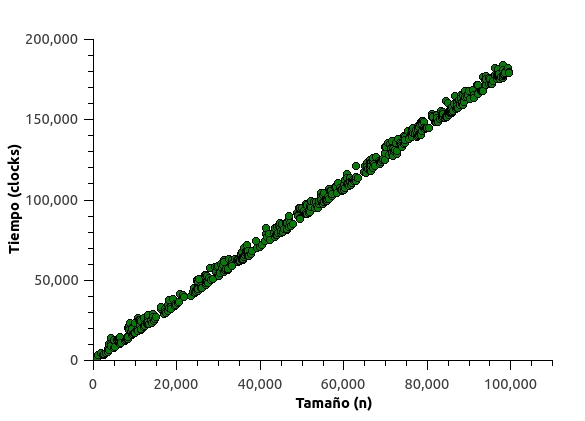
\includegraphics[scale=0.66]{imagenes/grafico1-1.jpg}
  \end{center}
\end{figure}

Si al tiempo medido lo dividimos por $log(n)$, se obtiene el siguiente resultado: 

\begin{figure}[H]
  \begin{center}
   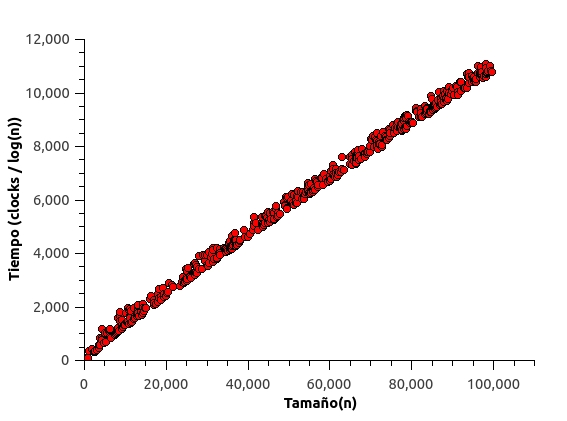
\includegraphics[scale=0.66]{imagenes/grafico1-2.jpg}
  \end{center}
\end{figure}

\newpage

Por ultimo, dividimos el ultimo resultado obtenido por $n$, para de esta manera constatar que la complejidad experimental coincide con la calculada teóricamente:

\begin{figure}[H]
  \begin{center}
   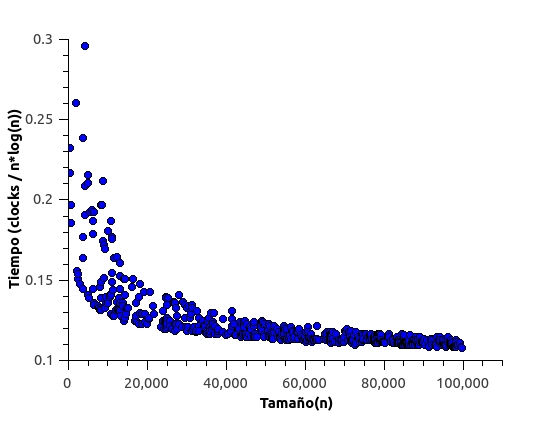
\includegraphics[scale=0.66]{imagenes/grafico1-3.jpg}
  \end{center}
\end{figure}

A continuación, adjuntamos una tabla con los últimos 20 valores obtenidos en las instancias aleatorias, teniendo en cuenta que los casos fueron previamente ordenados según el tamaño ($n$):

\begin{table}[H]
\parbox{0.3\textwidth}{
    \begin{tabular}{ | l | l |l | l |}
    \hline
	Tamaño($n$) & Tiempo($t$) & \textbf{$t / log(n)$} & \textbf{$t / n*log(n)$} \\ \hline
96,553	&	178,384	&	10,772.61	&	0.112	\\ \hline
96,631	&	176,000	&	10,627.89	&	0.110	\\ \hline
96,703	&	181,731	&	10,973.25	&	0.113	\\ \hline
96,714	&	176,870	&	10,679.63	&	0.110	\\ \hline
96,750	&	178,210	&	10,760.19	&	0.111	\\ \hline
96,998	&	177,114	&	10,691.63	&	0.110	\\ \hline
97,107	&	179,106	&	10,810.82	&	0.111	\\ \hline
97,288	&	175,469	&	10,589.58	&	0.109	\\ \hline
97,538	&	176,710	&	10,662.09	&	0.109	\\ \hline
97,904	&	176,177	&	10,626.46	&	0.109	\\ \hline
98,066	&	184,153	&	11,105.95	&	0.113	\\ \hline
98,068	&	177,755	&	10,720.08	&	0.109	\\ \hline
98,100	&	181,413	&	10,940.38	&	0.112	\\ \hline
98,229	&	178,379	&	10,756.18	&	0.110	\\ \hline
98,296	&	178,935	&	10,789.07	&	0.110	\\ \hline
98,404	&	180,022	&	10,853.57	&	0.110	\\ \hline
98,612	&	179,711	&	10,832.83	&	0.110	\\ \hline
99,097	&	182,861	&	11,018.01	&	0.111	\\ \hline
99,342	&	179,873	&	10,835.65	&	0.109	\\ \hline
99,482	&	179,194	&	10,793.42	&	0.108	\\ \hline
    \textbf{Promedio} & & & 0.110 \\ \hline

    \end{tabular}
%   \caption*{Ver Apendice A para Tabla com-pleta}
}
\end{table}

\textbf{Promedio de las 500 instancias}: 0.125
\\
\\
A partir de la información suministrada, podemos concluir que, en el último resultado, estamos en presencia de una constante cercana a 0, pero distinta a 0. Si bien esta conclusión no es suficiente como demostración matemática de que el limite no tiende a 0, si efectivamente tiende a 0, esto no afecta la conclusión a la que arribamos, ya que la complejidad sigue siendo $\mathcal{O}(n*log(n))$
De este análisis se desprende que la complejidad calculada teóricamente coincide con la complejidad de la experimentación.


\subsubsection{Experimentación con instancias particulares}
La diferencia entre mejor o peor caso viene dado por el algoritmo de ordenamiento, ya que es la operación con mayor complejidad, $\mathcal{O}(n*log(n))$. En la implementación presentada se utiliza la función   \texttt{std::sort}\footnote{Referencia:  \url{http://en.cppreference.com/w/cpp/algorithm/sort}}, que acorde a la documentación disponible\footnote{Referencia:  \url{https://gcc.gnu.org/onlinedocs/libstdc++/libstdc++-html-USERS-4.4/a01027.html}}, la complejidad es siempre la misma. Por lo cual carece de sentido plantear mejor y peor caso, ya que el resultado sería el mismo.

Para demostrar este argumento, planteamos el siguiente experimento:
\begin{itemize}
	\item Casos donde las ciudades ya están ordenadas desde el input, según el costo de salvar cada ciudad de forma creciente (posible ``mejor'' caso). Para generar este tipo de input, fijamos la cantidad de soldados y costo de enviar refuerzos de cada ciudad, mientras vamos incrementando de ciudad en ciudad los zombis en las mismas de forma que necesitamos cada vez mas soldados para rescatar la ciudad.
    \begin{codesnippet}
Ejemplo:
5 ciudades, $ XX presupuesto (es irrelevante)
ciudad 1: 1000 zombis 100 soldados $ 10 costo p/soldado
ciudad 2: 2000 zombis 100 soldados $ 10 costo p/soldado
ciudad 3: 3000 zombis 100 soldados $ 10 costo p/soldado
ciudad 4: 4000 zombis 100 soldados $ 10 costo p/soldado
ciudad 5: 5000 zombis 100 soldados $ 10 costo p/soldado
\end{codesnippet}
	\item Casos donde las ciudades ya están ordenadas desde el input, según el costo de salvar cada ciudad de forma decreciente (posible ``peor'' caso). Para generar este tipo de input, fijamos la cantidad de soldados y costo de enviar refuerzos de cada ciudad, mientras vamos decrementando de ciudad en ciudad los zombis en las mismas de forma que necesitamos cada vez menos soldados para rescatar la ciudad.

\begin{codesnippet}
Ejemplo:
5 ciudades, $ XX presupuesto (es irrelevante)
ciudad 1: 5000 zombis 100 soldados $ 10 costo p/soldado
ciudad 2: 4000 zombis 100 soldados $ 10 costo p/soldado
ciudad 3: 3000 zombis 100 soldados $ 10 costo p/soldado
ciudad 4: 2000 zombis 100 soldados $ 10 costo p/soldado
ciudad 5: 1000 zombis 100 soldados $ 10 costo p/soldado
\end{codesnippet}
    \item 100 instancias de cada tipo.
\end{itemize}

A continuación exponemos gráficamente el resultado de la experimentación:

\begin{figure}[H]
        \centering
        \begin{subfigure}[b]{0.5\textwidth}
                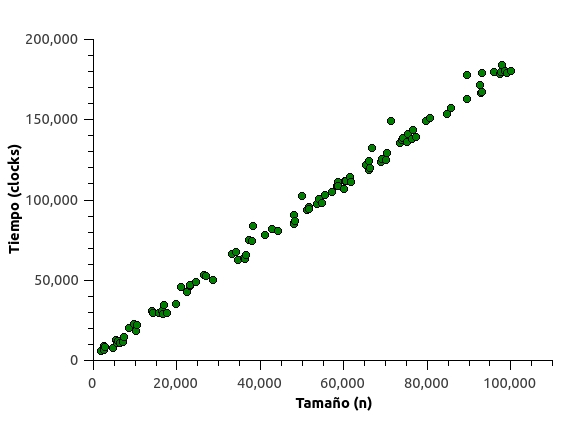
\includegraphics[width=\textwidth]{imagenes/grafico1-mejor1.jpg}
                \caption{Mejor Caso}
        \end{subfigure}%
        ~ %add desired spacing between images, e. g. ~, \quad, \qquad, \hfill etc.
          %(or a blank line to force the subfigure onto a new line)
        \begin{subfigure}[b]{0.5\textwidth}
                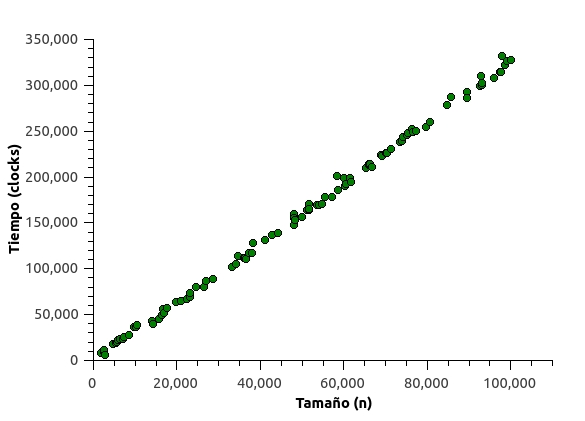
\includegraphics[width=\textwidth]{imagenes/grafico1-peor1.jpg}
                \caption{Peor Caso}
        \end{subfigure}

\end{figure}

Al igual que en el caso de las instancias aleatorias, dividimos por $log(n)$ a los tiempos obtenidos:

\begin{figure}[H]
        \centering
        \begin{subfigure}[b]{0.5\textwidth}
                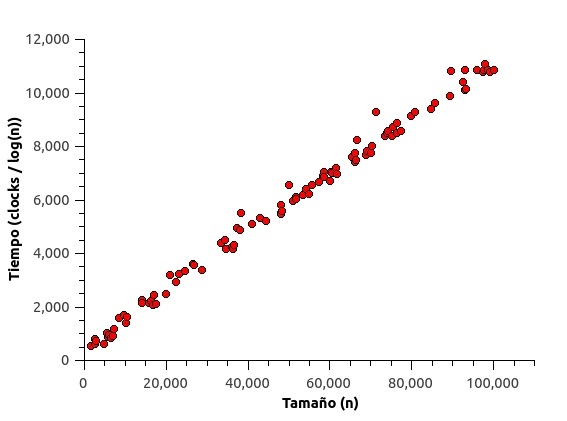
\includegraphics[width=\textwidth]{imagenes/grafico1-mejor2.jpg}
                \caption{Mejor Caso}
        \end{subfigure}%
        ~ %add desired spacing between images, e. g. ~, \quad, \qquad, \hfill etc.
          %(or a blank line to force the subfigure onto a new line)
        \begin{subfigure}[b]{0.5\textwidth}
                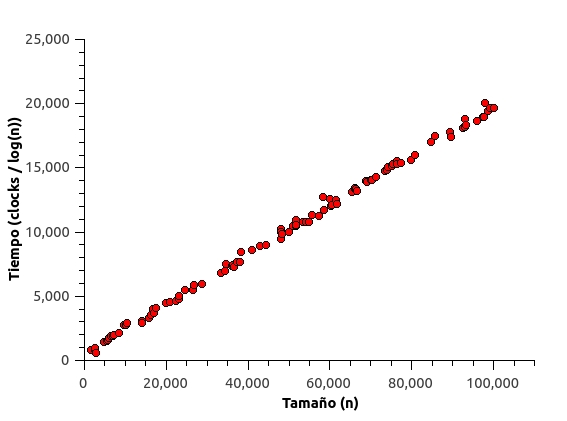
\includegraphics[width=\textwidth]{imagenes/grafico1-peor2.jpg}
                \caption{Peor Caso}
        \end{subfigure}

\end{figure}

Por último dividimos el anterior resultado por $n$:

\begin{figure}[H]
        \centering
        \begin{subfigure}[b]{0.5\textwidth}
                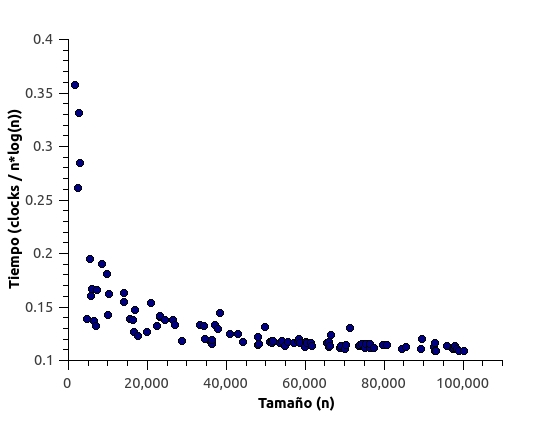
\includegraphics[width=\textwidth]{imagenes/grafico1-mejor3.jpg}
                \caption{Mejor Caso}
        \end{subfigure}%
        ~ %add desired spacing between images, e. g. ~, \quad, \qquad, \hfill etc.
          %(or a blank line to force the subfigure onto a new line)
        \begin{subfigure}[b]{0.5\textwidth}
                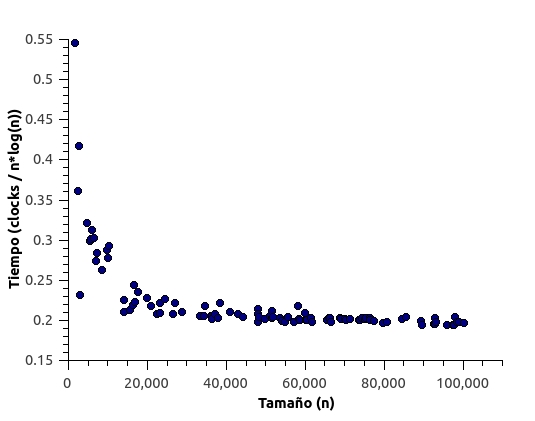
\includegraphics[width=\textwidth]{imagenes/grafico1-peor3.jpg}
                \caption{Peor Caso}
        \end{subfigure}

\end{figure}

Visualmente queda en evidencia la similitud entre ambos casos y el resultado obtenido con las instancias aleatorias. De esta forma, demostramos la inexistencia de un mejor o peor caso práctico.

A continuación, adjuntamos una tabla con los últimos 20 valores obtenidos en las instancias consideradas ``mejor''  caso, teniendo en cuenta que los casos fueron previamente ordenados según el tamaño ($n$):

\begin{table}[H]
\parbox{0.3\textwidth}{
    \begin{tabular}{ | l | l |l | l |}
    \hline
	Tamaño($n$) & Tiempo($t$) & \textbf{$t / log(n)$} & \textbf{$t / n*log(n)$} \\ \hline
75,298	&	141,520	&	8,735.63	&	0.116	\\ \hline
76,191	&	138,505	&	8,540.55	&	0.112	\\ \hline
76,329	&	144,175	&	8,888.75	&	0.116	\\ \hline
77,184	&	139,809	&	8,611.04	&	0.112	\\ \hline
79,597	&	149,414	&	9,177.52	&	0.115	\\ \hline
80,640	&	151,454	&	9,292.11	&	0.115	\\ \hline
84,521	&	154,040	&	9,411.61	&	0.111	\\ \hline
85,486	&	157,776	&	9,630.24	&	0.113	\\ \hline
89,272	&	163,195	&	9,923.13	&	0.111	\\ \hline
89,483	&	178,221	&	10,834.55	&	0.121	\\ \hline
92,479	&	171,924	&	10,421.63	&	0.113	\\ \hline
    \end{tabular}
  \caption*{Tabla 1/2}
}
\end{table}
\begin{table}[H]
\parbox{0.3\textwidth}{
    \begin{tabular}{ | l | l |l | l |}
    \hline
	Tamaño($n$) & Tiempo($t$) & \textbf{$t / log(n)$} & \textbf{$t / n*log(n)$} \\ \hline

92,854	&	167,048	&	10,122.48	&	0.109	\\ \hline
92,877	&	179,340	&	10,867.09	&	0.117	\\ \hline
93,021	&	167,888	&	10,171.78	&	0.109	\\ \hline
95,888	&	180,248	&	10,891.73	&	0.114	\\ \hline
97,401	&	179,004	&	10,801.82	&	0.111	\\ \hline
97,567	&	180,332	&	10,880.35	&	0.112	\\ \hline
97,863	&	184,156	&	11,108.14	&	0.114	\\ \hline
98,415	&	180,447	&	10,879.09	&	0.111	\\ \hline
98,914	&	179,276	&	10,803.74	&	0.109	\\ \hline
100,032	&	180,844	&	10,887.59	&	0.109	\\ \hline
    \textbf{Promedio} & & & 0.113 \\ \hline

    \end{tabular}
  \caption*{Tabla 2/2}
}
\end{table}
\textbf{Promedio de las 100 instancias}: 0.133
\\
\\
La información de los últimos 20 valores obtenidos en las instancias consideradas ``peor'' caso son:

\begin{table}[H]
\parbox{0.3\textwidth}{
    \begin{tabular}{ | l | l |l | l |}
    \hline
	Tamaño($n$) & Tiempo($t$) & \textbf{$t / log(n)$} & \textbf{$t / n*log(n)$} \\ \hline
75,298	&	248,304	&	15,327.10	&	0.204	\\ \hline
76,191	&	252,415	&	15,564.52	&	0.204	\\ \hline
76,329	&	249,327	&	15,371.63	&	0.201	\\ \hline
77,184	&	250,608	&	15,435.32	&	0.200	\\ \hline
79,597	&	254,918	&	15,657.94	&	0.197	\\ \hline
80,640	&	261,103	&	16,019.37	&	0.199	\\ \hline
84,521	&	279,177	&	17,057.29	&	0.202	\\ \hline
85,486	&	287,561	&	17,551.97	&	0.205	\\ \hline
89,272	&	293,204	&	17,828.37	&	0.200	\\ \hline
89,483	&	286,589	&	17,422.54	&	0.195	\\ \hline
92,479	&	299,692	&	18,166.63	&	0.196	\\ \hline
92,854	&	310,673	&	18,825.61	&	0.203	\\ \hline
92,877	&	300,995	&	18,238.77	&	0.196	\\ \hline
93,021	&	303,404	&	18,382.25	&	0.198	\\ \hline
95,888	&	309,010	&	18,672.36	&	0.195	\\ \hline
97,401	&	314,691	&	18,989.72	&	0.195	\\ \hline
97,567	&	315,383	&	19,028.66	&	0.195	\\ \hline
97,863	&	332,936	&	20,082.43	&	0.205	\\ \hline
98,415	&	322,493	&	19,443.00	&	0.198	\\ \hline
98,914	&	327,398	&	19,730.04	&	0.199	\\ \hline
100,032	&	327,654	&	19,726.19	&	0.197	\\ \hline
    \textbf{Promedio} & & & 0.199 \\ \hline

    \end{tabular}
%   \caption*{Ver Apendice A para Tabla com-pleta}
}
\end{table}

\textbf{Promedio de las 100 instancias}: 0.223
\\
\\


% \begin{figure}[H]
%   \begin{center}
%    \includegraphics[scale=0.66]{imagenes/grafico2-1.png}
%   \end{center}
% \end{figure}




\newpage
\section{Ejercicio 2 - Alta frecuencia}
\begin{figure}[h]
\begin{center}
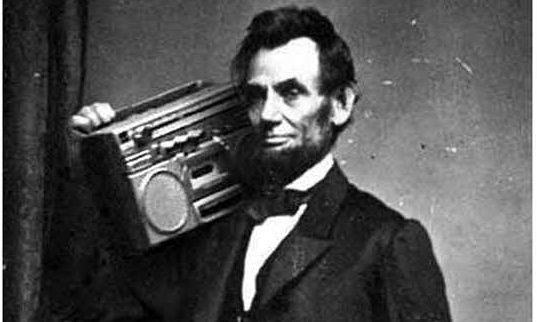
\includegraphics[width=0.6\textwidth] {imagenes/frecuencia.jpeg}
\end{center}
\end{figure}

\subsection{Problema a resolver}
Se tienen una lista de frecuencias que transmiten señales, donde cada una tiene un tiempo de inicio y fin y un costo por transmisión. El problema a resolver consiste en dar un algoritmo que minimice los costos, es decir, que para cada unidad de tiempo encuentre la frecuencia con menor costo e indique como ir cambiando de frecuencia acorde pasa el tiempo. A la vez, queremos transmitir todo el tiempo que sea posible.\\

\smallskip
Tenemos los siguientes parámetros de entrada:
	\begin{itemize}[noitemsep,nolistsep]
      \item $n$ = Cantidad de frecuencias
	  \item Luego vienen $n$ líneas con frecuencias, donde $F_{i}$ representa a la frecuencia en la línea $i$ con $1 \leq i \leq n$ y tiene los siguientes parámetros:
      \begin{itemize}
      \item $c_{i}$ = Costo de la frecuencia
      \item $b_{i}$ = Tiempo de inicio de la frecuencia
      \item $e_{i}$ = Tiempo de final de la frecuencia
      \end{itemize}
  	\end{itemize}
\smallskip

\begin{itemize}
\item Ejemplo: Situación inicial.

\begin{codesnippet}
2
10 1 16
5 6 10
\end{codesnippet}

Aquí se presentan dos señales, la primera tiene costo 10, inicio 1 y fin 16. La segunda tiene costo 5, inicio 6 y fin 10.

En este caso el algoritmo debe elegir la mejor señal para los tiempos 1 al 16.

En este ejemplo tenemos $n$ = 2 y luego $n$ señales:

\begin{table}[H]
\centering
\parbox{0.3\textwidth}{
    \begin{tabular}{ | l | l | l | l |}
    \hline
$F_{i}$ & $c_{i}$ & $b_{i}$ & $e_{i}$ \\ \hline
$F_{1}$ & 10 & 1 & 16 \\ \hline
$F_{2}$ & 5 & 6 & 10 \\ \hline
    \end{tabular}
}
\end{table}

\item Solución del ejemplo:

\begin{codesnippet}
130
1 1 6
2 6 10
1 10 16
\end{codesnippet}

La solución muestra que lo mejor es usar la primera señal de los tiempos 1 al 6, luego pasar a la segunda del 6 al 10 para, finalmente, retornar a la primer señal del 10 al 16.

El costo total de la transmisión anterior es 130 que es el menor costo posible para el ejemplo.

\end{itemize}

\subsection{Resolución planteada}

La solución planteada utiliza la técnica de \textit{Divide and Conquer}.
En este caso, se agregan todas las frecuencias recibidas a un vector y luego se llama a una función que se queda con dos problemas de menor complejidad en cada paso. Se llama a la misma recursivamente hasta llegar al caso base y luego se van uniendo las soluciones parciales hasta alcanzar un único vector con la solución final. \\


Veamos ahora como hacemos para unir dos soluciones parciales. En primer lugar, creo un indice de iteración para cada uno de los dos vectores que contienen los elementos que quiero unir (los llamamos vector izq y der):

\begin{codesnippet}
int izq_it <- 0
int der_it <- 0
\end{codesnippet}

Mientras ambos iteradores sean menores al tamaño del vector que itera, me fijo cual de los dos elementos a los que apuntan tiene menor principio y llamo a la función auxiliar $mergeAux$ que los irá agregando al resultado según corresponda. Es importante ver cual tiene menor principio porque queremos transmitir todo el tiempo posible.

\begin{codesnippet}
izq y der son Vector<Signal>
    donde Signal es tupla <numero:int, costo:int, principio:int, final:int>
Mientras izq_it < |izq| y der_it < |der| hacer:
    Si izq[izq_it].principio <= der[det_it].principio:
        mergeAux(izq, der, izq_it, der_it, result)
    Sino
        mergeAux(der, izq, der_it, izq_it, result)
    Fin if
Fin ciclo
\end{codesnippet}

Una vez que sale del ciclo, significa que al menos uno de los vectores fue recorrido completamente, por lo que nos queda agregar los elementos restantes del otro vector al vector solución:

\begin{codesnippet}
Mientras izq_it < |izq| hacer:
    result.agregarAlFinal(izq[izq_it])
    izq_it <- izq_it + 1
Fin ciclo

Mientras der_it < |der| hacer:
    result.agregarAlFinal(der[der_it])
    der_it <- der_it + 1
Fin ciclo
\end{codesnippet}

\vspace{1em}

Como vimos en el pseudocódigo arriba, la función auxiliar $mergeAux$ necesita comparar dos señales que pertencen una al vector $izq$ y la otra a $der$. Para hacer esto utiliza los iteradores pasados por parametro.\\

Pasamos a mostrar cómo la función auxiliar mergeAux compara dos señales dadas. Sean $F_{1}$ y $F_{2}$ las dos señales pertenecientes a $izq$ y $der$ apuntadas por los iteradores,  donde $b_{1} < b_{2}$. Sea también $resultado$ un vector que contendra frecuencias.\\

Al comparar las dos señales se nos presentan varios casos posibles:\\

\textit{Observacion:} Para todos los gráficos siguientes, las señales azules representan las de menor costo y las rojas las de mayor. Además, la que se encuentra más a la izquierda representa a $F_{1}$. \\
\\

\begin{itemize}
	\item Si $c_{1} \leq c_{2}$:
        \begin{itemize}
            \item Si $b_{2} \geq e_{1}$, entonces agrego $F_{1}$ a $resultado$ y aumento el iterador del vector al que pertenece $F_{1}$.
            \begin{figure}[H]
        		\centering
				\begin{subfigure}[b]{0.25\textwidth}
                	
\includegraphics[width=\textwidth]{imagenes/ej2-a.jpg}
                	\caption*{Lo llamaremos caso A}
        		\end{subfigure}%
			\end{figure}
            \item Si $b_{2} \leq e_{1} \land e_{1} < e_{2}$. Entonces, agrego $F_{1}$ a $resultado$, defino $b_{2} = e_{1}$ y aumento el iterador del vector al que pertenece $F_{1}$.

            \begin{figure}[H]
        	\centering
				\begin{subfigure}[b]{0.25\textwidth}
                	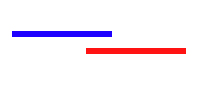
\includegraphics[width=\textwidth]{imagenes/ej2-b2.jpg}
                	\caption*{Lo llamaremos caso B}
        		\end{subfigure}%

				\begin{subfigure}[b]{0.25\textwidth}
                	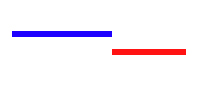
\includegraphics[width=\textwidth]{imagenes/ej2-b3c.jpg}
                	\caption*{$b_{2} = e_{1}$}
        		\end{subfigure}%
			\end{figure}
            \item Si $b_{2} \leq e_{1} \land e_{1} \geq e_{2}$. Entonces desestimo $F_{2}$, es decir, aumento el iterador del vector al que pertece $F_{2}$.
            \begin{figure}[H]
        		\centering
				\begin{subfigure}[b]{0.25\textwidth}
                	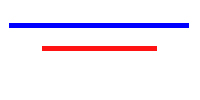
\includegraphics[width=\textwidth]{imagenes/ej2-c.jpg}
                	\caption*{Lo llamaremos caso C}
        		\end{subfigure}%
			\end{figure}
        \end{itemize}

	\item Si $c_{1} > c_{2}$:\\

\begin{itemize}
            \item Si $b_{2} \leq e_{1} \land e_{1} > e_{2}$. Entonces defino $F_{1}^{\prime} = F_{1}$ pero con $e_{1}^{\prime} = b_{2}$ y la agrego a $resultado$. Si $e_{2} < e_{1}$, entonces defino $b_{1} = e_{2}$ y no aumento ningún iterador.
            \begin{figure}[H]
        		\centering
				\begin{subfigure}[b]{0.25\textwidth}
                	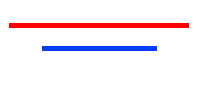
\includegraphics[width=\textwidth]{imagenes/ej2-c2.jpg}
                	\caption*{Lo llamaremos caso C$^{\prime}$}
        		\end{subfigure}%

				\begin{subfigure}[b]{0.25\textwidth}
                	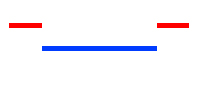
\includegraphics[width=\textwidth]{imagenes/ej2-c3.jpg}
                	\caption*{Aquí el primer segmento rojo es $F_{1}^{\prime}$ y el segundo $F_{1}$}
        		\end{subfigure}%
			\end{figure}

            \item Si $b_{2} \leq e_{1} \land e_{1} \leq e_{2}$. Entonces defino $e_{1} = b_{2}$ y agrego $F_{1}$ a $resultado$ y aumento el iterador del vector al que pertenece $F_{1}$.

            \begin{figure}[H]
        		\centering
				\begin{subfigure}[b]{0.25\textwidth}
                	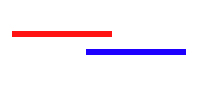
\includegraphics[width=\textwidth]{imagenes/ej2-b.jpg}
                	\caption*{Lo llamaremos caso B$^{\prime}$}
        		\end{subfigure}%

				\begin{subfigure}[b]{0.25\textwidth}
                	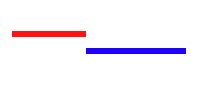
\includegraphics[width=\textwidth]{imagenes/ej2-b4c.jpg}
                	\caption*{$e_{1} = b_{2}$}
        		\end{subfigure}%
			\end{figure}

            \item Si $b_{2} \geq e_{1}$. Entonces agrego $F_{1}$ a $resultado$ y aumento el iterador del vector al que pertenece $F_{1}$.
            \begin{figure}[H]
        		\centering
				\begin{subfigure}[b]{0.25\textwidth}
                	
\includegraphics[width=\textwidth]{imagenes/ej2-a2.jpg}
                	\caption*{Lo llamaremos caso A$^{\prime}$}
        		\end{subfigure}%
			\end{figure}
        \end{itemize}

        Notemos que el único caso donde no se aumenta ninguno de los dos iteradores es el caso C$^{\prime}$. Sin embargo, como podemos ver en ese caso, luego de ejecutar ese llamado a $mergeAux$ nos queda nada más y nada menos que el caso A, y aumenta en uno nuestra cantidad de señales. \\ 
Por lo tanto al ejecutar un $merge$ entero con una entrada de tamaño $k$, donde $k$ es la suma de la cantidad de elementos de los dos vectores a unir, necesitamos a lo sumo $2k$ operaciones  Y se duplica la cantidad de señales retornadas, que es a lo sumo $2k$.\\ 

Por lo que podemos decir que $merge$ tiene complejidad lineal en la cantidad de elementos. \\

\end{itemize}

Ahora, veamos que si $n$ es la entrada del problema, el vector resultante luego de hacer el algoritmo tendrá a lo sumo tamaño $2n$
\begin{lemma}
Sea $n$ la cantidad de frecuencias recibidas al comienzo del problema. La cantidad de frecuencias resultantes al dar el menor costo de transmisión será a lo sumo $2n$.
\end{lemma}

\begin{proof}

Supongamos que puedo graficar en una línea de tiempo todos los $t$ que tienen comienzos y finales de las $n$ señales. De esta forma tendré $n$ comienzos y $n$ finales graficados a lo sumo porque dos señales pueden compartir los mismos comienzos o finales.\\

Por ejemplo:

            \begin{figure}[H]
        		\centering
				\begin{subfigure}[b]{0.5\textwidth}
azul                	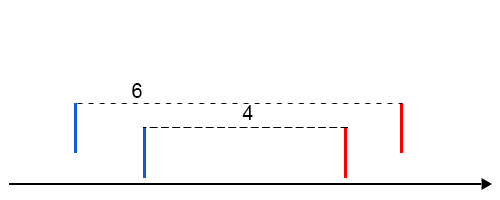
\includegraphics[width=\textwidth]{imagenes/demo1.jpg}
                	\caption*{Aqui podemos ver 2 frecuencias, por ende 2 comienzos (azul) y 2 finales (rojo)}
        		\end{subfigure}%
			\end{figure}

Como vimos arriba, solo se da en el caso C$^{\prime}$ que al comparar dos frecuencias me terminan quedando tres. Pero observemos que siempre que una frecuencia es separada en fragmentos, estos están delimitados por el comienzo o el final de otra frecuencia. Es decir, pondré como final de un fragmento el comienzo de otro, o pondré como comienzo de un fragmento el final de otro. \\

            \begin{figure}[H]
        		\centering
				\begin{subfigure}[b]{0.5\textwidth}
                	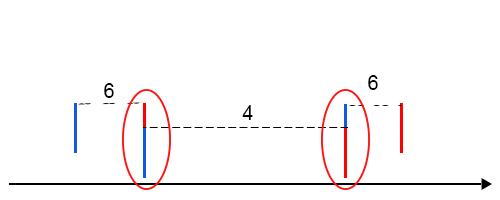
\includegraphics[width=\textwidth]{imagenes/demo2.jpg}
                	\caption*{Aqui podemos ver que aunque aumenta la cantidad de frecuencias, siguen usando los mismos comienzos y finales}
        		\end{subfigure}%
			\end{figure}


Pero como ya dijimos, en una entrada de tamaño $n$, tengo $n$ comienzos y $n$ finales. Entonces, la cantidad de veces que puedo cortar una frecuencia en dos está acotada por la cantidad de comienzos y finales que yo tenga, y estos son $2n$.
\end{proof}


%Por lo tanto, aunque una ejecución de $merge$ con un subproblema de tamaño $k$ con $k \leq n$ , donde $k$ es la suma de la cantidad de elementos de los dos vectores a unir, puede devolvernos $2k$ frecuencias, el tamaño total de la solución para todo el problema está acotado por $2n$.

Por lo tanto, aunque vimos que $merge$ puede retornar para una entrada $k$ algo de a lo sumo tamaño $2k$, donde $k$ es la suma de la cantidad de elementos de los dos vectores a unir. Uno puede pensar que cuando se ejecutan los $merge$ de nuestro algoritmo divide and conquer, se puede duplicar el tamaño de las frecuencias que devuelve en cada paso y aumentar de manera exponencial, esto es falso ya que estas están acotadas por $2n$.

\subsection{Complejidad propuesta}

Analizamos la complejidad usando Teorema Maestro\footnote{Thomas H. Cormen, Charles E. Leiserson, Ronald L. Rivest, and Clifford Stein. Introduction to Algorithms. The MIT Press, 2001.}:

Sean $a > 1$ y $b > 1$ constantes, sea $f(n)$ una función y sea
$T(n)$ definido en los enteros no negativos por la
recurrencia
$$T(n)= aT(\frac{n}{b}) + f(n)$$
$T(n)$ puede ser acotado asintóticamente de la siguiente manera: \\

1) Si $f(n) = \mathcal{O}(n^{\log_b a-\epsilon})$ para alguna constante $\epsilon > 0$, entonces, $T(n) = \Theta (n^{\log_b a})$. \\

2) Si $f(n) = \mathcal{O}(n^{\log_b a})$ entonces, $T(n) = \Theta (\log_b a  \log n )$. \\

3) Si $f(n) = \Omega (n^{\log_b a + \epsilon})$ para alguna constante $\epsilon > 0$ y si,
$af(\frac{n}{b}) \leq cf(n)$ para alguna constante $c < 1$ y todas las $n$ suficientemente grandes, entonces $T(n) = \Omega (f(n))$. \\

	% WAITTTTTT, no viste (en ningun lado lo dijiste) que el merge tiene complejidad lineal. Lo único que viste es que el tamaño total de la solución resultante está acotado por 2n. CUIDADO. ARREGLAR. WARNING.
	% OTRA COSA, quizas te creería más que las operaciones además del merge son constante si antes de esta demo de Complejidad hubiera un pseudocodigo, aunque se que era largo el pseudocodigo de este problema, fijate si le encontras alguna vuelta (no es tan importante esto que digo).
En cada paso nos quedamos con dos subproblemas que tienen la mitad de tamaño que el original, así que $a$ = 2 y $c$ = 2. Además de la recursión, se unen los resultados. Para esto llamamos a la función merge, que ya vimos que tiene complejidad lineal en la cantidad de elementos del arreglo. Más allá de esto, se hace una cantidad constante de comparaciones y asignaciones, por lo que podemos decir que $f(n)$  $\in$  $\Theta
(n)$. No podríamos usar el primer caso del teorema, porque $n^{\log_2 2-\epsilon}$ = $n^{1 - \epsilon}$ , y no es cierto que $f(n) \in$  $\Theta$ ($n^{1 - \epsilon}$ ). En cambio, podemos usar el segundo caso, porque como ya dijimos $f(n)$ $\in$ $\Theta (n)$ . Reemplazando, obtenemos $T(n)$ $\in$
 $\Theta$ ( $n^{\log_2 2}$  $log (n)$), o sea $T(n) \in$  $\Theta$ ($n$  $log (n)$).

\newpage
\subsection{Implementación en C++}
\lstinputlisting[language=C++]{codigo/ej2.cpp}

\subsection{Experimentación computacional}
La función que utilizamos para llevar a cabo las mediciones fue \texttt{std::clock}\footnote{Referencia \url{http://en.cppreference.com/w/cpp/chrono/c/clock}}. La unidad temporal que utilizamos para este ejercicio fue de nanosegundos.
La complejidad teórica calculada es de $\mathcal{O}(n*log(n))$

\subsubsection{Experimentación con instancias aleatorias}
Para generar las instancias aleatorias utilizamos la función \texttt{std::rand}\footnote{Referencia \url{http://en.cppreference.com/w/cpp/numeric/random/rand}} con determinados intervalos de valores para la variables, para obtener instancias coherentes. El detalle de intervalos es el siguiente:
\begin{itemize}
	\item Cantidad de muestras: 100
	\item Cantidad de frecuencias ($n$): de 1 a 3000
    \item Costos ($P$): 1 $\leq P \leq$ 10.000
	\item Para cada frecuencia, se verifico que su tiempo final fuera mayor que su inicio (no se usaron frecuencias invalidas).
\end{itemize}

Entonces, para cada $n$, del 1 al 3000 se generaron 100 instancias aleatorias de tamaño $n$.
Luego, estas fueron promediadas, arrojando los siguientes resultados:

\begin{figure}[H]
        \centering
        \begin{subfigure}[b]{0.5\textwidth}
                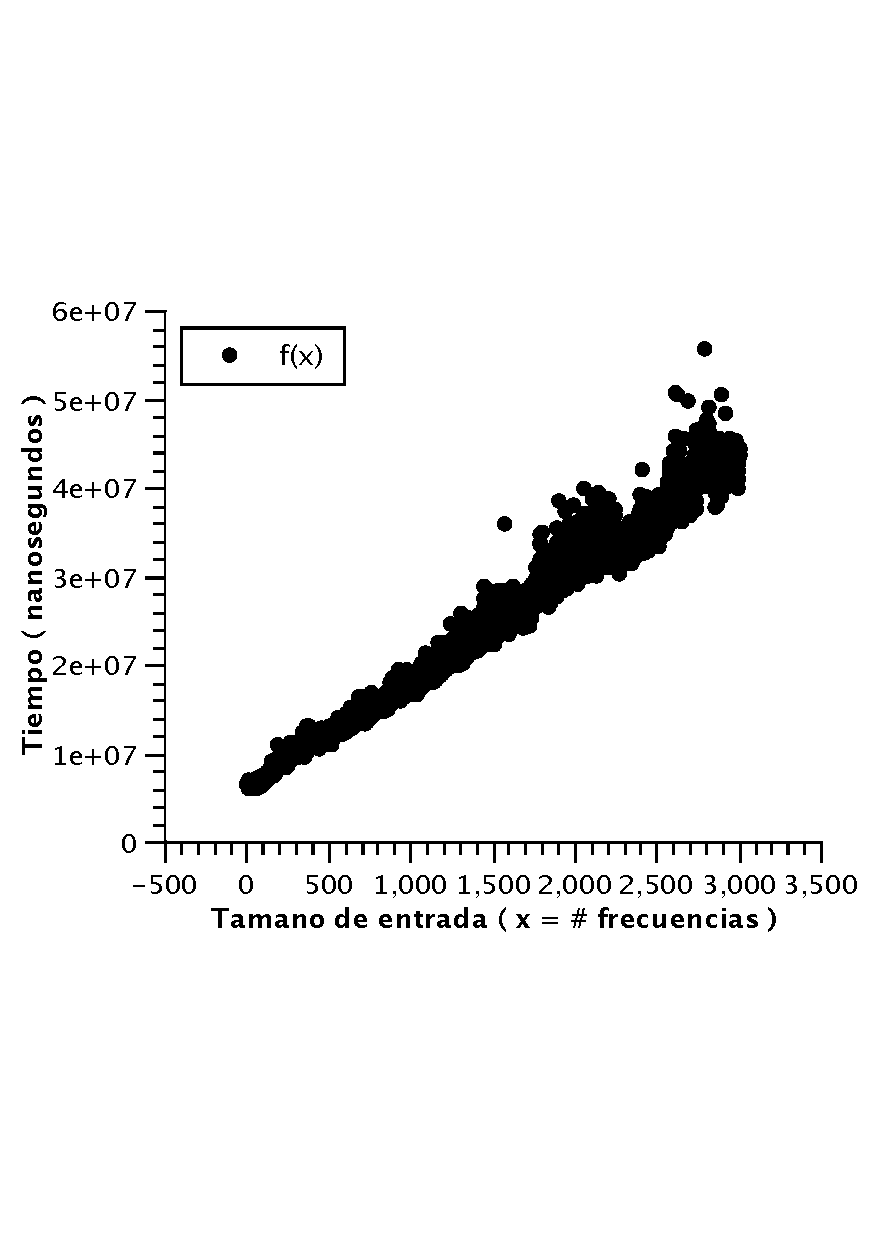
\includegraphics[width=\textwidth]{imagenes/af-rand-nlogn.pdf}
                \caption*{Tiempos sin procesar}
        \end{subfigure}%
\end{figure}

\begin{figure}[H]
        \centering
        \begin{subfigure}[b]{0.5\textwidth}
                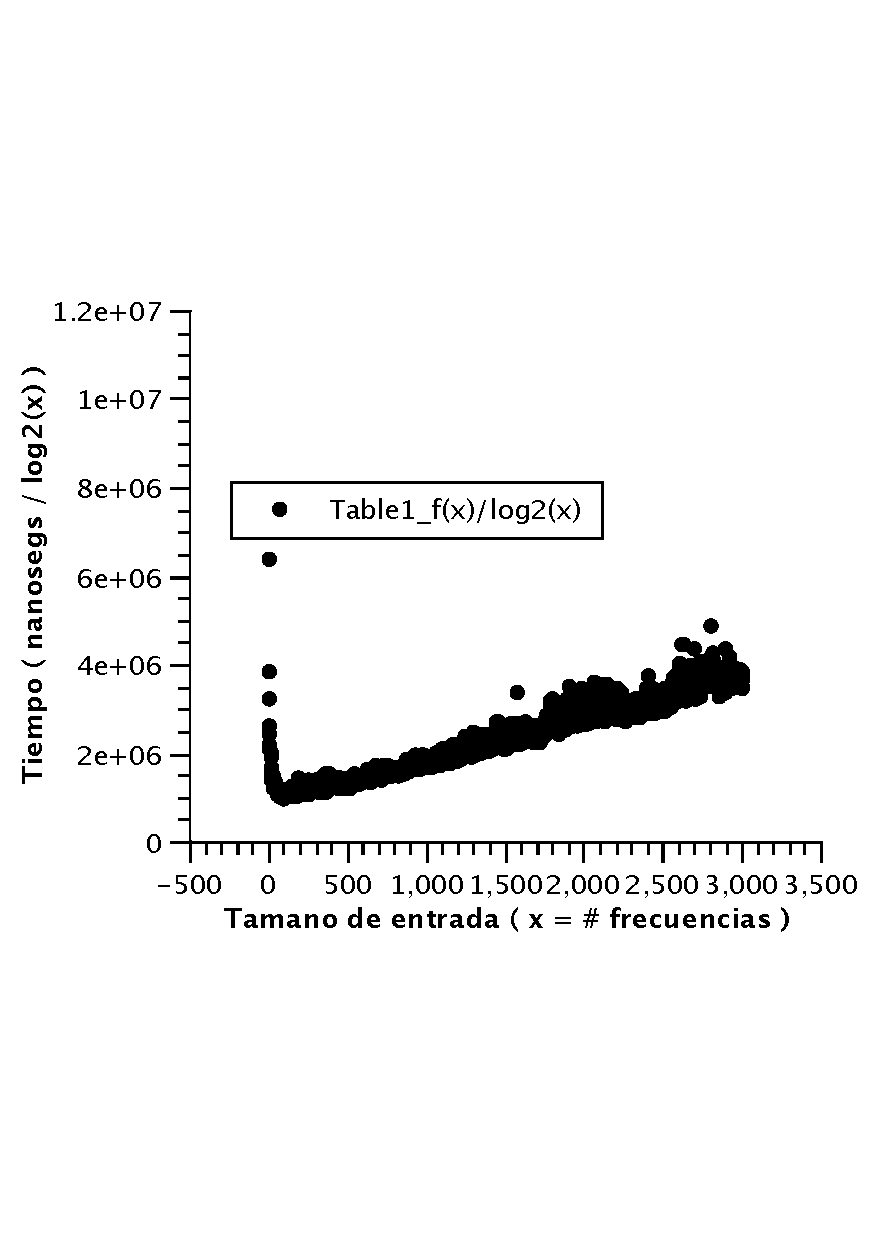
\includegraphics[width=\textwidth]{imagenes/af-rand-lineal.pdf}
                \caption*{Dividiendo a los tiempos por $\log(n)$}
        \end{subfigure}
\end{figure}

\begin{figure}[H]
        \centering
        \begin{subfigure}[b]{0.5\textwidth}
                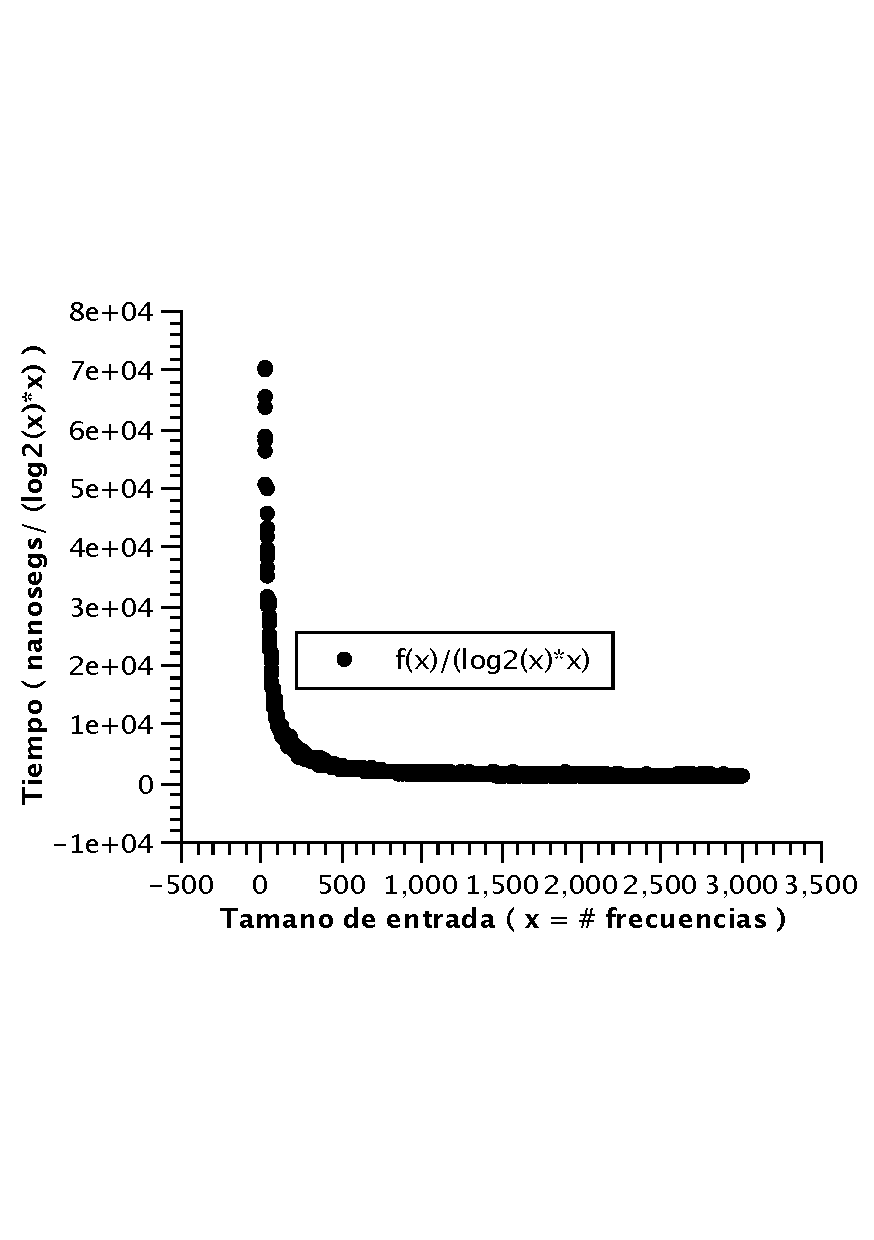
\includegraphics[width=\textwidth]{imagenes/af-rand-const.pdf}
                \caption*{Dividiendo a los tiempos por $n \log(n)$}
        \end{subfigure}
\end{figure}


A continuación, adjuntamos una tabla con los ultimos 20 valores obtenidos en este último paso, teniendo en cuenta que los casos fueron previamente ordenados segun el tamaño ($n$):

\begin{table}[H]
\parbox{0.3\textwidth}{
    \begin{tabular}{ | l | l | l | l |}
    \hline
Tamano($n$) & Tiempo($t$) & $t / log(n)$ & $t / n*log(n)$ \\ \hline
2,980 & 41,823,717 & 3,623,894.53913547 & 1,216.07199299848 \\ \hline
2,981 & 42,205,634 & 3,656,833.08407709 & 1,226.713547157695 \\ \hline
2,982 & 41,379,610 & 3,585,113.377975757 & 1,202.251300461354 \\ \hline
2,983 & 42,125,330 & 3,649,569.318887776 & 1,223.456023763921 \\ \hline
2,984 & 45,341,672 & 3,928,055.705472136 & 1,316.372555453129 \\ \hline
2,985 & 40,887,769 & 3,542,055.278169351 & 1,186.618183641324 \\ \hline
2,986 & 42,795,296 & 3,707,146.720857472 & 1,241.509283609334 \\ \hline
2,987 & 43,971,377 & 3,808,865.466588621 & 1,275.147461194717 \\ \hline
2,988 & 41,832,598 & 3,623,449.707752226 & 1,212.667238203556 \\ \hline
2,989 & 41,938,501 & 3,632,470.907368039 & 1,215.279661213797 \\ \hline
2,990 & 41,182,479 & 3,566,839.555032387 & 1,192.922928104477 \\ \hline
2,991 & 43,525,502 & 3,769,612.695656072 & 1,260.318520781034 \\ \hline
2,992 & 42,113,000 & 3,647,127.818332012 & 1,218.959832330218 \\ \hline
2,993 & 42,931,618 & 3,717,867.670108657 & 1,242.187661245792 \\ \hline
2,994 & 43,479,759 & 3,765,179.403366345 & 1,257.574951024163 \\ \hline
2,995 & 42,626,427 & 3,691,130.148415261 & 1,232.430767417449 \\ \hline
2,996 & 42,621,659 & 3,690,563.361166947 & 1,231.830227358794 \\ \hline
2,997 & 40,046,500 & 3,467,438.573756513 & 1,156.969827746584 \\ \hline
2,998 & 40,993,661 & 3,549,300.88989128 & 1,183.88955633465 \\ \hline
2,999 & 44,504,732 & 3,853,134.875349259 & 1,284.806560636632 \\ \hline
3,000 & 43,832,216 & 3,794,751.699991118 & 1,264.917233330373 \\ \hline
    \end{tabular}
}
\end{table}

A partir de la información suministrada, podemos observar que, en el primer gráfico las mediciones tienden a algo un poco más grande que lineal. Al dividir los tiempos por logaritmo de $n$ (segundo gráfico), se observa que tienden a ser algo lineal. Por último, en el último gráfico, se dividen además de por logaritmo de $n$, por $n$ y el gráfico que arroja es constante y mayor a 0. Por lo que podemos concluir que la complejidad de $\mathcal{O}(n*log(n))$ se condice con nuestra predicción de complejidad.

\subsubsection{Experimentación con instancias particulares}


Como quedo demostrado en la justificación de la complejidad teórica, el peor caso ocurre cuando al comparar dos frecuencias la de menor costo esta completamente contenida dentro de la de mayor costo. En este caso, la salida termina teniendo $2n-1$ señales. \\

\begin{figure}[H]
        		\centering
				\begin{subfigure}[b]{0.25\textwidth}
                	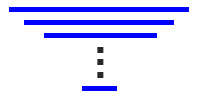
\includegraphics[width=\textwidth]{imagenes/ej2-wc-dibujo.jpg}
                	\caption{Aquí supongamos que cada señal tiene costo menor que la de arriba}
        		\end{subfigure}%
			\end{figure}

Generamos una muestra de peor caso de tamaños 1 a 3000 de la siguiente manera:
\begin{itemize}
	\item El costo de la primer frecuencia es 3001
	\item El comienzo de la primer frecuencia es 1
    \item El final de la primer frecuencia es 6001
    \item Cada frecuencia que se agrega disminuye en 1 el costo, aumenta en 1 el comienzo y disminuye en 1 el final
\end{itemize}



\begin{figure}[H]
        \centering
        \begin{subfigure}[b]{0.5\textwidth}
                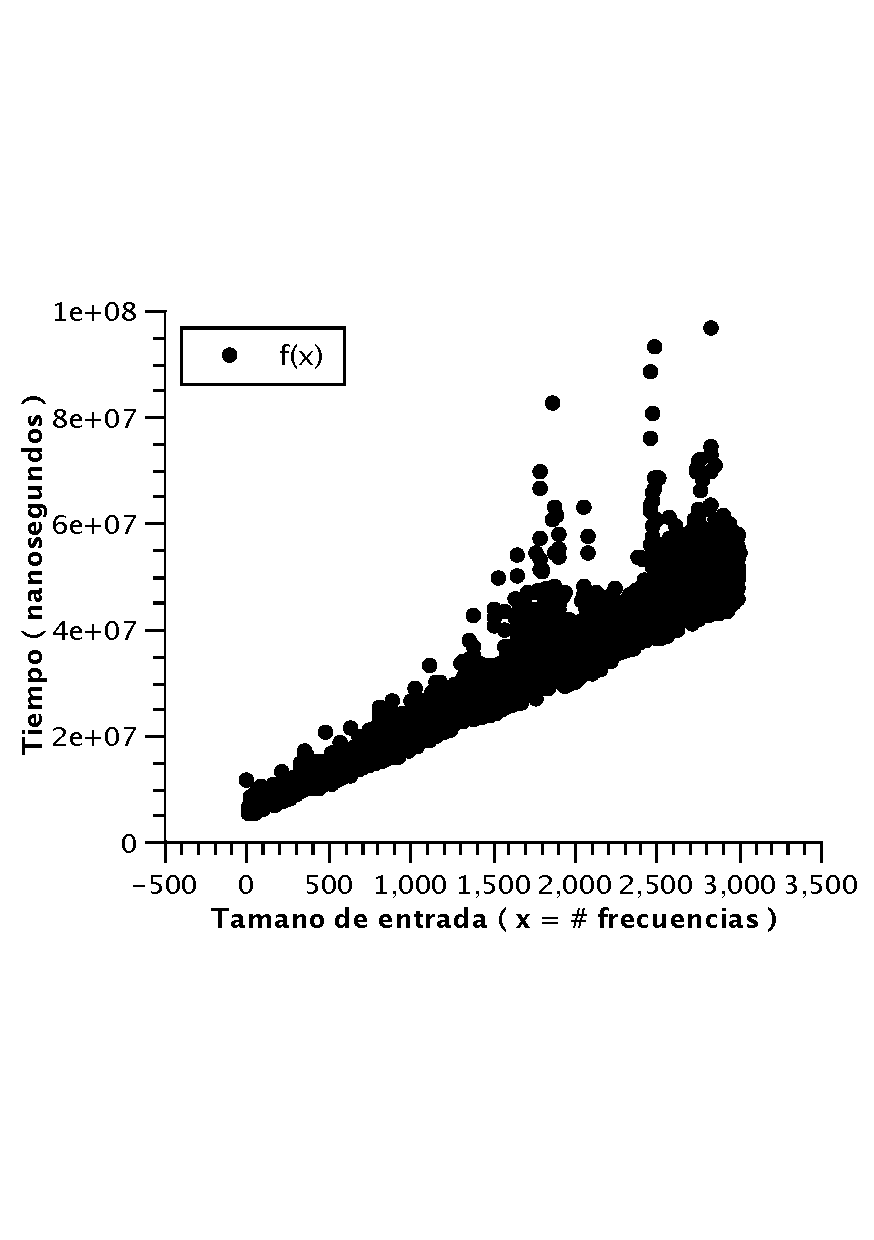
\includegraphics[width=\textwidth]{imagenes/af-wc-nlogn.pdf}
                \caption*{Tiempos sin procesar}
        \end{subfigure}%
\end{figure}

\begin{figure}[H]
        \centering
        \begin{subfigure}[b]{0.5\textwidth}
                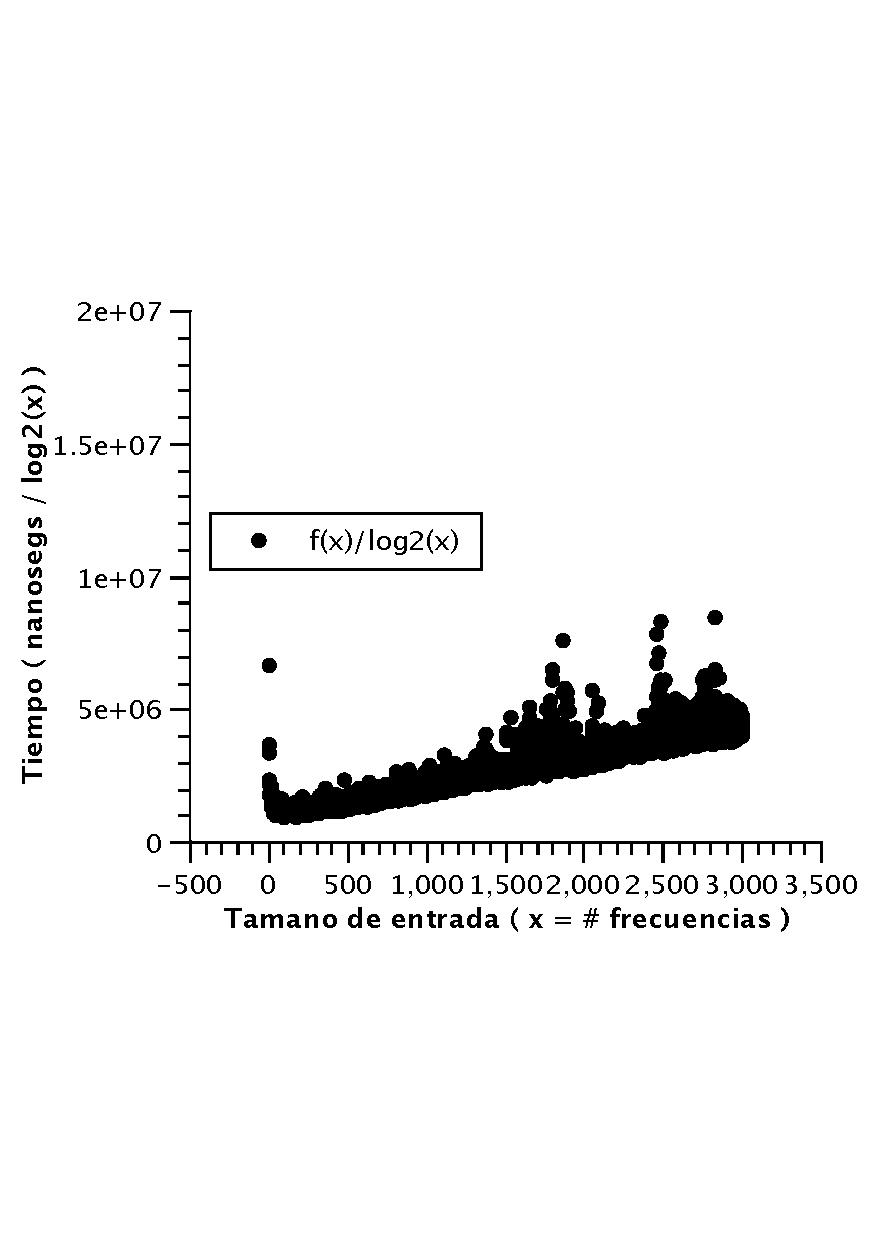
\includegraphics[width=\textwidth]{imagenes/af-wc-lineal.pdf}
                \caption*{Dividiendo a los tiempos por $\log(n)$}
        \end{subfigure}
\end{figure}

\begin{figure}[H]
        \centering
        \begin{subfigure}[b]{0.5\textwidth}
                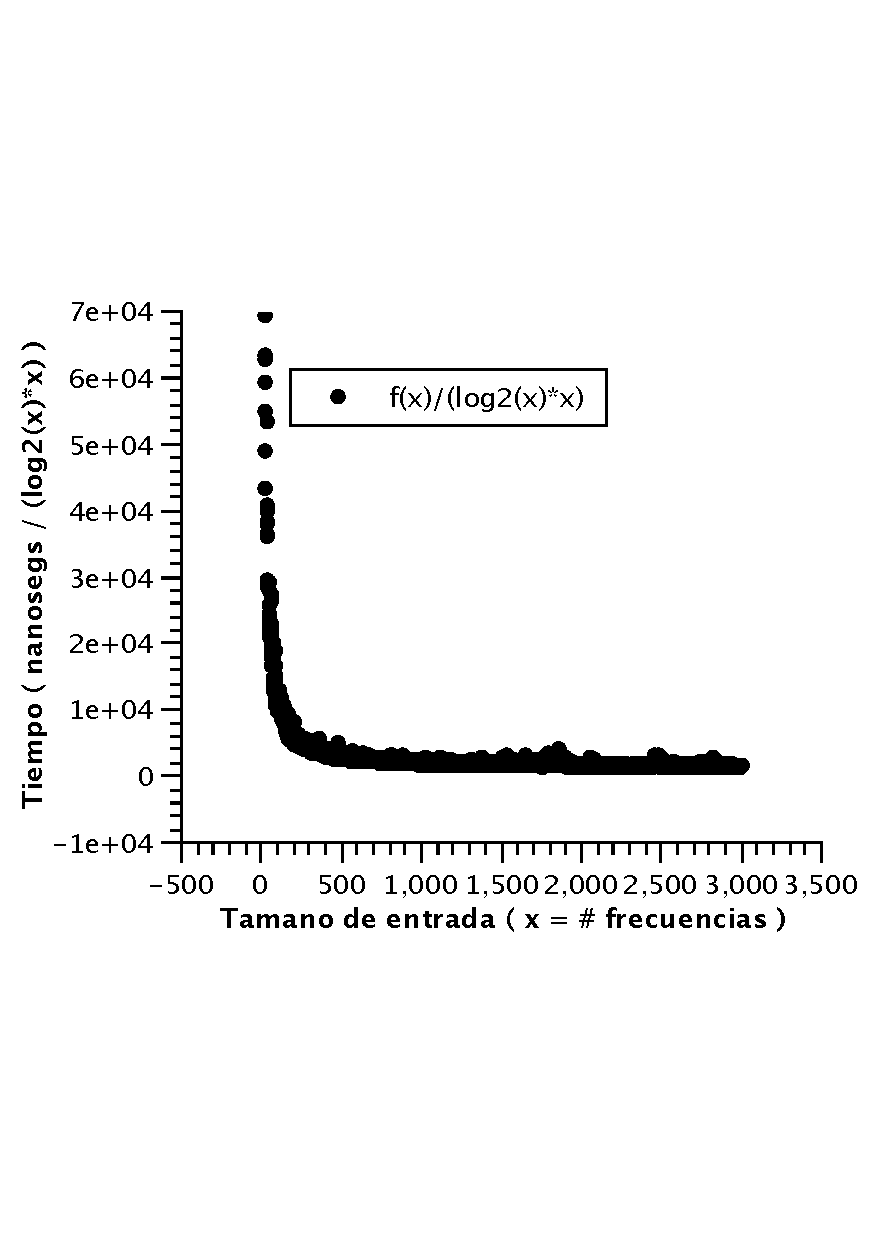
\includegraphics[width=\textwidth]{imagenes/af-wc-const.pdf}
                \caption*{Dividiendo a los tiempos por $n \log(n)$}
        \end{subfigure}
\end{figure}

A continuación, adjuntamos una tabla con los ultimos 20 valores obtenidos en este último paso, teniendo en cuenta que los casos fueron previamente ordenados segun el tamaño ($n$):

\begin{table}[H]
\parbox{0.3\textwidth}{
    \begin{tabular}{ | l | l | l | l |}
    \hline
Tamano($n$) & Tiempo($t$) & $t / log(n)$ & $t / n*log(n)$ \\ \hline
2,980 & 47,188,711 & 4,088,754.524179232 & 1,372.065276570212 \\ \hline
2,981 & 48,174,802 & 4,174,021.169127874 & 1,400.208376091202 \\ \hline
2,982 & 47,537,404 & 4,118,622.264314194 & 1,381.161054431319 \\ \hline
2,983 & 50,090,561 & 4,339,644.926021389 & 1,454.792130748035 \\ \hline
2,984 & 50,262,066 & 4,354,321.012249329 & 1,459.222859332885 \\ \hline
2,985 & 50,960,628 & 4,414,654.205912404 & 1,478.946132633971 \\ \hline
2,986 & 51,054,247 & 4,422,579.162716796 & 1,481.104876998257 \\ \hline
2,987 & 58,162,121 & 5,038,088.62161512 & 1,686.671784939779 \\ \hline
2,988 & 53,436,807 & 4,628,581.344801059 & 1,549.056674966887 \\ \hline
2,989 & 57,760,600 & 5,002,889.805053413 & 1,673.767080981403 \\ \hline
2,990 & 50,334,133 & 4,359,469.874376941 & 1,458.016680393625 \\ \hline
2,991 & 52,002,106 & 4,503,745.849466659 & 1,505.765914231581 \\ \hline
2,992 & 55,619,141 & 4,816,805.175903654 & 1,609.894778042665 \\ \hline
2,993 & 53,321,719 & 4,617,647.88796729 & 1,542.815866343899 \\ \hline
2,994 & 49,501,380 & 4,286,628.55316679 & 1,431.739663716362 \\ \hline
2,995 & 48,025,112 & 4,158,615.939924299 & 1,388.519512495592 \\ \hline
2,996 & 51,954,186 & 4,498,656.781775029 & 1,501.554333035724 \\ \hline
2,997 & 51,590,387 & 4,466,969.595815528 & 1,490.48034561746 \\ \hline
2,998 & 45,924,717 & 3,976,240.104930008 & 1,326.297566687795 \\ \hline
2,999 & 54,525,123 & 4,720,681.230346652 & 1,574.085105150601 \\ \hline
    \end{tabular}
}
\end{table}

A partir de la información suministrada, podemos observar que, en el primer gráfico las mediciones tienden a algo un poco más grande que lineal. Al dividir los tiempor por $\log(n)$ (segundo gráfico) se observa que el gráfico tiende a ser lineal. Por último, al dividir los tiempos por $n \log(n)$, el gráfico que arroja es constante y mayor a 0. Aunque este es peor caso, los gráficos siguen mostrando que se cumple la complejidad teórica calculada. Por lo que podemos concluir que la complejidad de $\mathcal{O}(n*log(n))$ se condice con nuestra predicción de complejidad.

\subsection{Adicionales}

Debido a un aumento en la demanda de nuestro servicio de transmisión de información, hemos duplicado
nuestro caudal de datos a transmitir y por tal motivo podemos ahora utilizar dos frecuencias en paralelo
en lugar de una sola. Quisiéramos resolver el mismo problema que antes pero ahora queremos transmitir
siempre que sea posible en dos frecuencias. En los momentos en que esto no sea posible, seguiremos
transmitiendo por una sola frecuencia, y obviamente en los momentos en los que esto último no se pueda
no transmitiremos nada. Es decir, el objetivo es transmitir información durante todo el tiempo que sea
posible y en la mayor cantidad de frecuencias en paralelo hasta un máximo de dos frecuencias, y hacer
esto invirtiendo la menor cantidad de dinero. Se pide desarrollar los siguientes puntos:

\begin{enumerate}
	\item \textit{Dar una idea de qué cambiaría en su algoritmo para resolver este nuevo problema.}

        Podríamos resolver este problema modificando el algoritmo que ya tenemos de la siguiente forma:

        Ejecutamos el algoritmo normalmente, pero guardando una copia extra del vector original que contiene a las señales, llamémosla $copia$.

        Una vez que se termina de ejecutar el algoritmo original, tendremos en el vector $resultado$ la opción de menor costo para la transmisión de las señales.

        Ahora, lo que se debe hacer es recorrer el vector $resultado$ y, por cada señal en $resultado$, buscar en el vector $copia$ la misma o el fragmento de la misma correspondiente y eliminarla.\\

        Esta tarea la haremos de la siguiente manera. Llamemos $R_{i}$ a la frecuencia en la posición $i$ de $resultado$. Buscamos en $copia$ la frecuencia correpondiente a $R_{i}$, llamemosla $C_{R_{i}}$. Actuaremos de la siguiente forma:

        Recordemos que dada una frecuencia $F_{i}$, $c_{i}$, $b_{i}$ y $e_{i}$ representan su costo, tiempo de comienzo y tiempo de fin respectivamente.
        \begin{itemize}

          \item Si $b_{i} = b_{R_{i}} \land e_{i} = e_{R_{i}}$ entonces esta señal se usa completamente, por lo que definimos $c_{R_{i}} = e_{R_{i}} = b_{R_{i}} = -1$.

          \item  Si $b_{i} > b_{R_{i}} \land e_{i} < e_{R_{i}}$ entonces me quedan dos fragmentos que no fueron usados, por lo que agrego al final de $copia$ una frecuencia $F$ con $c = c_{R_{i}}$, $b = b_{R_{i}}$ y $e = e_{i}$. Luego modifico a $C_{R_{i}}$ definiendole $b_{R_{i}} = b_{i}$.

          \item Si $b_{i} > b_{R_{i}} \land e_{i} = e_{R_{i}}$ o $b_{i} = b_{R_{i}} \land e_{i} < e_{R_{i}}$ entonces modifico $b_{R_{i}} = b_{i}$ o $e_{R_{i}} = e_{i}$ según sea necesario.

		\end{itemize}

		Una vez finalizado esto, podríamos tener frecuencias que tengan todos sus atributos en -1 (primer caso arriba), por lo que debemos crear otro vector, llamemoslo $v$ y lo llenaremos con los elementos de $copia$ que no tengan todo en -1. Luego, ejecutamos nuevamente el algoritmo de $mergeSort$ que usamos para resolver el ejercicio original sobre el vector $v$, obteniendo así las segundas mejores señales. \\

		\item \textit{¿Cómo afectaría este cambio en la complejidad temporal de su algoritmo?}

    Veamos: el agregado que le hacemos a nuestro algoritmo se divide en tres partes, una es crear el vector $copia$, la segunda es seleccionar las señales en $resultado$ y eliminar los fragmentos correspondientes en $copia$ y la tercera es volver a correr el algoritmo $mergeSort$ original sobre $copia$.

    Crear $copia$ no modifica nuestra complejidad temporal ya que lo hacemos al mismo tiempo que creamos el vector original.

    Sabemos que $resultado$ tiene tamaño de a lo sumo $2n-1$. Deberíamos recorrerlo entero y, por cada frecuencia, buscar el correspondiente en $copia$. Esto parece tener complejidad $\mathcal{O}(n^2)$. Sin embargo, podemos hacer algunos cambios en nuestra estructura para poder hacer esto de manera más eficiente.\\

    Actualmente tenemos la siguiente estructura $Signal$ en la implementación: \\

            \begin{codesnippet}
struct Signal {
    Signal() : numero(0), costo(0), principio(0), fin(0) {};
    Signal(const int n,const int c,const int p, const int f) : numero(n),
    costo(c), principio(p), fin(f) {};

    int numero;
    int costo;
    int principio;
    int fin;
};
\end{codesnippet}

	Notemos que estamos guardando el número de señal, que es ni más ni menos que el orden con que la señal fue guardada tanto en el vector original como en $copia$. Por esto, cada vez que ejecutando el algoritmo tengamos que buscar una señal de $resultado$ en $copia$, podemos hacerlo en $\mathcal{O}(1)$. Luego tenemos que modificarlo según sea necesario, esto lo hacemos también en $\mathcal{O}(1)$. Por lo que todo el proceso de recorrer $resultado$ y modificar $copia$ podemos hacerlo en $\mathcal{O}(2n) \in \mathcal{O}(n)$ porque vimos que $resultado$ tiene su tamaño acotado por $2n$. \\

   Ahora tenemos que crear el vector $v$ y llenarlo con las señales de $copia$ que cumplen las condiciones que vimos en el punto anterior. Esto esta acotado por el tamaño de $copia$ luego de modificarlo.

   Veamos cual es el tamaño de $copia$ viendo cuales son los tres casos posibles al comparar una señal de $resultado$ con una de copia:

           Llamemos $R_{i}$ a la frecuencia en la posición $i$ de resultado. Buscamos en $copia$ la frecuencia correpondiente a $R_{i}$, llamemosla $C_{R_{i}}$. Actuaremos de la siguiente forma: \\

        Recordemos que dada una frecuencia $F_{i}$, $c_{i}$, $b_{i}$ y $e_{i}$ representan su costo, tiempo de comienzo y tiempo de fin respectivamente.
        \begin{itemize}

          \item Si $b_{i} = b_{R_{i}} \land e_{i} = e_{R_{i}}$ entonces esta señal se usa completamente, por lo que definimos $c_{R_{i}} = e_{R_{i}} = b_{R_{i}} = -1$. \\

En este caso, el tamaño de $copia$ se mantiene igual, ya que no se agregan fragmentos. \\

          \item  Si $b_{i} > b_{R_{i}} \land e_{i} < e_{R_{i}}$ entonces me quedan dos fragmentos que no fueron usados, por lo que agrego al final de $copia$ una frecuencia $F$ con $c = c_{R_{i}}$, $b = b_{R_{i}}$ y $e = e_{i}$. Luego modifico a $C_{R_{i}}$ definiendole $b_{R_{i}} = b_{i}$. \\

En este caso, el tamaño de $copia$ aumenta en uno. \\
Recordemos que $resultado$ está ordenado cronologicamente por lo tanto mientras lo vaya recorriendo, cada frecuencia $R_{i}$ tendrá $b_{i} \geq e_{i-1}$. Entonces, al partir las frecuencias, la que agrego al final de $copia$ tiene que ser la que tenga el menor final ya que nunca volverá a ser buscada, mientras que la otra debe permanecer en su lugar, para que si tiene que volver a ser accedida en el futuro, esto se logre en $\mathcal{O}(1)$.\\ 


          \item Si $b_{i} > b_{R_{i}} \land e_{i} = e_{R_{i}}$ o $b_{i} = b_{R_{i}} \land e_{i} < e_{R_{i}}$ entonces modifico $b_{R_{i}} = b_{i}$ o $e_{R_{i}} = e_{i}$ según sea necesario. \\

          En este caso, el tamaño de $copia$ se mantiene igual, ya que no se agregan fragmentos. \\


\end{itemize}
Entonces, como podemos ver, el tamaño de $copia$ aumenta a lo sumo en uno por cada iteración. Esto se ejecuta tantas veces como elementos tenga $resultado$ y ya vimos que el tamaño de resultado está acotado por $2n$ por lo que $copia$ finaliza con a lo sumo $3n$ elementos. Por lo tanto, crear $v$ nos cuesta $\mathcal{O}(3n) \in \mathcal{O}(n)$\\

Por último, solo tenemos que correr nuestro $mergeSort$ con entrada $v$, como ya demostramos en el ejercicio original esto tiene complejidad $\mathcal{O}(n\log(n))$. Entonces con $v$ quedaría $\mathcal{O}(3n\log(3n)) \in \mathcal{O}(n\log(n))$. \\

Por lo tanto, no se modifica la complejidad del algoritmo, ya que esta termina siendo igualmente de:

$$\mathcal{O}(n\log(n))$$

\end{enumerate}


\subsection{Informe de modificaciones}
    \begin{itemize}
    \item Mejoras en descripción del problema.
    \item La resolución del problema fue modificada completamente.
    \item Aclaraciones sobre Teorema Maestro en la justificación de la complejidad.
    \item Aclaraciones sobre como fueron tomadas las muestras.
    \item Agregados los adicionales
\end{itemize}

\newpage
\section{Ejercicio 3 - El sen\~or de los caballos}
\begin{figure}[h]
\begin{center}
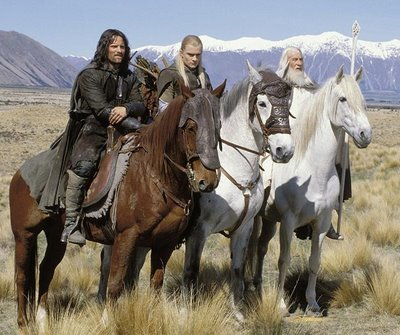
\includegraphics[width=0.6\textwidth] {imagenes/caballos.jpeg}
\end{center}
\end{figure}

\subsection{Problema a resolver}
El problema a resolver consiste en dar un algoritmo de Backtracking que minimice la cantidad de caballos utilizados para cubrir todos los casilleros de un tablero de $n$ x $n$.

Decimos que un casillero está cubierto sí está ocupado con un caballo o es amenazado por otro caballo.

A su vez, el tablero inicial puede o no tener caballos ya posicionados, en cuyo caso igual se quiere buscar la solución optima que minimice la cantidad de caballos utilizados.

\begin{itemize}
\item Ejemplo 1: Situación inicial.

\begin{codesnippet}
n = 8, sin caballos iniciales
\end{codesnippet}
\item Solución del ejemplo\footnote{Se puede encontrar las soluciones para $3 \leq n \leq 17$ con tableros vacios en \url{http://home.earthlink.net/~morgenstern/solution/knsols1.htm}}:

\begin{codesnippet}
Cantidad de caballos agregados: 12
Tablero:
0 0 0 0 0 0 0 0
0 0 1 0 0 0 0 0
0 0 1 1 0 1 1 0
0 0 0 0 0 1 0 0
0 0 1 0 0 0 0 0
0 1 1 0 1 1 0 0
0 0 0 0 0 1 0 0
0 0 0 0 0 0 0 0
\end{codesnippet}
\end{itemize}

\subsection{Resolución planteada}
La solución planteada utiliza la técnica algorítmica de backtracking, como se pide en el enunciado. La idea es recorrer el tablero inicial evaluando cada posición vacía (es decir sin caballo. Puede ser vacía y estar amenazada) para determinar si es necesario poner un caballo o, en caso contrario, comparar las mejores soluciones al poner un caballo en la casilla o dejarla como estaba.

Nuestro modelo consiste en representar el tablero con una matriz de tamaño $n*n$. De esta manera conseguimos acceder a cada dato del tablero en tiempo constante. Dicho esto, nuestro algoritmo va 'procesando' cada casilla sin caballo secuencialmente de izquierda a derecha y de arriba hacia abajo. Es decir que empieza desde la primer casilla sin un caballo (x,y), toma las decisiones correspondientes a la casilla, se fija si la casilla (x,y+1) tiene un caballo, si no lo tiene la 'procesa', en caso contrario se fija la casilla (x, y+2), (x, y+3), ... , (x, n-1) , (x+1, 0) , ... , (x+1, n-1) , (n-1, 0) y asi hasta (n-1, n-1).

Para ayudar a tomar estas decisiones hemos pensado e implementado una serie de \textit{podas} que evitan llegar a soluciones invalidas o (parcialmente) suboptimas. Consideramos que se va a llegar a una solución invalida cuando, al visitar una casilla sin caballo que no esta amenazada, no ponerle un caballo implica que no pueda ser amenazada en el futuro. Es decir que no hay habría manera de colocar un caballo en una casilla a ser visitada en el futuro de manera que aquella casilla quede amenazada. De esto se encargan las podas 'B' y 'C', las cuales explicamos en la próxima sección. Las demás podas se encargan de no considerar decisiones que necesariamente llevarían a soluciones subóptimas (tableros en los cuales todas las casillas tienen un caballo o están amenazadas, pero cuya cantidad de caballos es mayor a la de otra solución).


\subsubsection{Poda A}
Este caso se da cuando todas las posiciones que amenaza el casillero siendo evaluado tienen un caballo o están amenazadas y alguna al menos tiene un caballo, es decir, la casilla actual esta amenazada.
Si pasa esto, entonces el casillero siendo evaluado tiene que permanecer vacío. Porque si pusiera un caballo, entonces me llevaría a una solución sub-optima, ya que estaría poniendo un caballo que no es realmente necesario.

\begin{itemize}
\item Notación: 'c' es el casillero siendo evaluado, 'a' son las posiciones amenazadas, '1' son las casillas que tienen un caballo.

\item Ejemplo: Situación inicial.

\begin{codesnippet}
Tablero (c es el casillero siendo evaluado):
c 0 a 0
0 0 a 0
0 1 0 0
0 0 0 1
\end{codesnippet}

\item Decisión subóptima:

\begin{codesnippet}
Tablero:
1 0 a 0
0 0 a 0
0 1 0 0
0 0 0 1
\end{codesnippet}

\item Decisión óptima:

\begin{codesnippet}
Tablero:
a 0 a 0
0 0 a 0
0 1 0 0
0 0 0 1
\end{codesnippet}
\end{itemize}

\subsubsection{Poda B}
Este caso se da cuando existe una posición que amenaza el casillero siendo evaluado que ya fue procesada, está vacía y solo la puede amenazar el casillero siendo evaluado (todas las otras posiciones que pueden amenazar a la amenazada ya fueron procesadas y ninguna tiene un caballo).
Si pasa esto, entonces el casillero siendo evaluado tiene que tener un caballo sí o sí. Dejarlo vacío me llevaría a una tablero incorrecto, porque sería imposible amenazar el otro casillero en el futuro.

\begin{itemize}
\item Ejemplo: Situación inicial.

\begin{codesnippet}
Tablero (c es el casillero siendo evaluado):
0 0 0 0
0 0 a 0
0 c 0 0
0 0 0 1
\end{codesnippet}

\item Decisión incorrecta:
en este caso, amenazar la casilla (0,0) se vuelve imposible

\begin{codesnippet}
Tablero:
0 0 0 0
0 0 a 0
0 a c 0
0 0 0 1
\end{codesnippet}

\item Decisión correcta:

\begin{codesnippet}
Tablero:
a 0 a 0
0 0 a a
0 1 c 0
0 0 0 1
\end{codesnippet}
\end{itemize}

\subsubsection{Poda C}
Este caso se da cuando todas las posiciones que amenaza el casillero siendo evaluado ya fueron procesadas y ninguna tiene un caballo.
Si pasa esto, entonces el casillero siendo evaluado tiene que tener un caballo sí o sí. Porque si se lo deja vacío, no hay forma de amenazarlo en el futuro.

\begin{itemize}
\item Ejemplo: Situación inicial.

\begin{codesnippet}
Tablero (c es el casillero siendo evaluado):
1 1 1
a c a
a a a
\end{codesnippet}

\item Decisión incorrecta:

\begin{codesnippet}
Tablero:
1 1 1
a 0 a
a a a
\end{codesnippet}

\item Decisión correcta:

\begin{codesnippet}
Tablero:
1 1 1
a 1 a
a a a
\end{codesnippet}
\end{itemize}

\subsubsection{Poda D}
Este caso se da cuando existe una posición que el casillero siendo evaluado amenaza que tiene un caballo, y a la vez, todas sus posiciones amenazadas que no son la actual tienen caballo. Además, no se deben cumplir \textit{B} o \textit{C}.
Si pasa esto, entonces el casillero siendo evaluado tiene que permanecer vacío, excepto que el caballo amenazado halla sido puesto a través del input. En caso contrario, si pusiera un caballo me llevaría a una solución sub-optima, porque el casillero amenazado, estaría siendo amenazado por todas las posiciones posibles y además tendría un caballo. Casos en los que una posición contiene un caballo y, a la vez, todas sus posiciones amenazadas contienen un caballo llevan a tableros subóptimos, porque poner un caballo allí no cambia el total de casillas amenazadas.

\begin{itemize}
\item Ejemplo: Situación inicial.

\begin{codesnippet}
Tablero (c es el casillero siendo evaluado):
c a 0 0
a 0 1 0
1 a a a
0 1 a 1
\end{codesnippet}

\item Solución parcial subóptima:

\begin{codesnippet}
Tablero:
1 a 0 0
a 0 1 0
1 a a a
0 1 a 1
\end{codesnippet}

\item Solución parcial óptima:

\begin{codesnippet}
Tablero:
a a 0 0
a 0 1 0
1 a a a
0 1 a 1
\end{codesnippet}
\end{itemize}

\subsubsection{Poda G}
Esta poda consiste en calcular una cota como primer aproximación a la cantidad de caballos necesarios para la solución óptima usando un \textit{algoritmo goloso}. Si en algún paso del algoritmo del ejercicio la cantidad de caballos supera esta cota, dejamos de calcular dicha solución, porque la solución que nos dio el algoritmo goloso es mejor (esto lo generaliza la poda Z).

La cota en cuestión se calcula antes de empezar el algoritmo de backtracking.

El algoritmo goloso que se utiliza para esta cota buscará en cada paso maximizar la cantidad de posiciones amenazadas al poner un caballo. Es decir, compara la cantidad de nuevas casillas amenazadas entre varios casilleros y se queda con la mejor, y asi recorre cada casilla del tablero una sola vez.

Como claramente este problema no adhiere al \textit{principio de optimalidad}, la solución dada no será óptima en principio, pero en general es una aproximación más interesante que usar como cota $n^2$.

\subsubsection{Poda S}
Esta poda funciona de manera muy parecida a lo que hace la \textit{Poda G}. Sin embargo, en este caso la cota a utilizar es la cantidad de caballos en la mejor solución que se conoce para un Tablero de ese tamaño (o sea, para un $n$ dado). Esta información fue recompilada del sitio mencionado en la sección de \textit{Problema a resolver} y tiene dichos valores para $3\leq n\leq 17$.

De esta forma, sí en algún momento encontramos una solución con cantidad de caballos igual a la cantidad de caballos utilizada en la solución optima, sabemos que no tenemos que seguir buscando y ya podemos dar la solución.

Es necesario notar, que los valores recompilados solo sirven para soluciones en las que el Tablero inicial esté vacío. Es por eso que esta poda además tiene en cuenta la cantidad de caballos iniciales. Sí en algún momento la solución parcial actual tiene más caballos que la solución optima más los caballos iniciales, entonces sabemos que podemos podar dicha solución, ya que no será optima.

\subsubsection{Poda Z}
Esta poda funciona de manera muy parecida a lo que hace la \textit{Poda G}. Sin embargo, en este caso la cota a utilizar es la cantidad de caballos en la mejor solución encontrada hasta el momento. De esta forma, una vez que nuestro algoritmo encuentre una solución de $k$ caballos, automaticamente empezara a podar todos los subarboles que tengan soluciones parciales con $k+1$ caballos.

\subsubsection{Pseudocódigo}
Para hacer el pseudocódigo más sencillo, no vamos a listar las condiciones que tienen que pasar para cada Poda, ya que cada una fue explicada más arriba con ejemplos.

\begin{codesnippet}
main:
	pongo tablero_inicial = un tablero vacio más los caballos pasados por input
	pongo cota_optima = resolver_con_goloso(tablero_inicial)
	result = resolver_aux(cota_optima, (0,0))

resolver_aux(optimo_alcanzado, ultima_celda):
	Si entro en los casos de las podas G, S o Z
		devuelvo la cantidad de caballos utilizados por la solución optima \
			alcanzada
	pongo siguiente = siguiente celda vacía sin un caballo en el tablero \
		después de ultima_celda
	Si no hay siguiente
		devuelvo el mínimo entre la cantidad de caballos usada por la \ 
			solución actual y la solución optima alcanzada
    Si entro en el caso de la poda A
		dejo la celda como esta y llamo a resolver_aux recursivamente
	Si entro en el caso de la poda B
		pongo un caballo en la celda y llamo a resolver_aux recursivamente
	Si entro en el caso de la poda C
		dejo la celda como esta y llamo a resolver_aux recursivamente
	Si entro en el caso de la poda D (y no entre en los casos B ni C)
		pongo un caballo en la celda y llamo a resolver_aux recursivamente
	Si no entre a ningún caso de poda
		pruebo llamando a resolver_aux recursivamente: dejando vacío y \
			poniendo un caballo en la celda
		devuelvo el mínimo de esos dos

resolver_con_goloso(tablero):
	pongo siguiente = siguiente celda vacia no amenazada en el tablero
    Si no hay siguiente
		devuelvo la cantidad de caballos usada
	pongo posibilidades = [las posibles formas de poner un caballo que haga
		que la celda "siguiente" este cubierta]
	tomo de posibilidades la que maximize la cantidad de celdas cubiertas
	agrego al tablero la decision tomada
	llamo resolver_con_goloso(tablero)

\end{codesnippet}

\subsubsection{Justificación}

Como planteamos en nuestra resolución, nuestro algoritmo primero encuentra una solución aproximada usando un algoritmo auxiliar goloso. Luego, procede visitando cada celda sin un caballo secuencialmente. Las podas desechan tableros incorrectos y decisiones que necesariamente llevarían a tableros con más caballos de lo necesario. Finalmente, si ninguna poda aplica, compara las soluciones dadas entre dejar un casillero vacío y poner un caballo en ese lugar.

\subsection{Complejidad propuesta}
Dado un Tablero de $n$ x $n$, el algoritmo propuesto evalúa cada celda de forma secuencial una sola vez, y ya que para cada celda hay dos posibilidades, o bien poner un caballo o bien dejarla vacía, el árbol de decisión tendría $2^{M}$ nodos, donde \textit{M} es la cantidad de celdas a evaluar.

Por ejemplo, en un tablero vacío de largo \textit{n}, $M= n^2$. Sin embargo, si el tablero inicial tiene k celdas con caballos ya cargados, entonces tenemos $M=n^2 - k$, pues hay $k$ celdas para las cuales no hay que decidir si tiene o no un caballo.

Ahora, para ver que el algoritmo propuesto tiene complejidad $\mathcal{O}(2^{n^2 - k})$, tenemos que ver que las operaciones realizadas en cada nodo (sin contar las llamadas recursivas y guardar un nuevo tablero, explicado a continuación) tienen costo constante. En nuestro caso, realizamos distintas comparaciones de enteros y checkeos para las podas. Estos checkeos, a su vez, consisten en recorrer las posiciones a las cuales amenazaría un caballo colocado en la posición actual. Como la cantidad de posiciones que un caballo puede amenazar es a lo sumo 8, podemos decir que este ciclo se repite una cantidad constante de veces. Dentro del ciclo, solo se realizan operaciones constantes. Por lo tanto, en cada paso, se realizan a lo sumo dos llamadas recursivas y operaciones de costo constante.

Cuando llegamos a soluciones del tablero con menos cantidad de caballos que la mejor solución calculada hasta el momento, queremos guardar el tablero para mostrar las casillas con caballo al final del algoritmo. Si bien esta operación tiene costo $n^2$, esto no sucede muy frecuentemente. Veamos lo siguiente: el tablero se guarda solo si se encuentra uno nuevo con menos cantidad de caballos que el mejor hasta ahora, pero las posibles cantidades de caballos en el tablero son de 0 a $n^2$. Por lo tanto, como tablero se guarda como máximo $n^2$ cantidad de veces y esta operación tiene un costo de $n^2$, guardar el tablero solo añade $n^4$ trabajo a todo el algoritmo (contando todo el árbol de recursión). Entonces, estos casos no le añaden complejidad al algoritmo ya que, en particular, $n^4$ esta en $\mathcal{O}(2^{n^2 - k})$.

Además, el algoritmo propuesto utiliza una función auxiliar que con un algoritmo goloso obtiene una primera cota para la solución optima. Entonces, tenemos que ver que la complejidad de esta función es a lo sumo $\mathcal{O}(2^{n^2 - k})$. Siguiendo la notación de antes, la función auxiliar tiene \textit{M} celdas a evaluar. Para cada una de ellas checkea si obtiene más celdas cubiertas amenazándola desde alguna celda vecina, o poniendo un caballo en ella, pero solo toma una decisión por cada celda y las evalúa secuencialmente. Como vimos recién, las comparaciones toman tiempo constante ya que cada celda tiene a lo sumo 8 celdas posibles que la pueden amenazar. Por lo tanto, la complejidad de esta función es $\mathcal{O}(M)$ que es estrictamente menor que $\mathcal{O}(2^{M})$.

Luego, la complejidad del algoritmo propuesto en el peor caso es:


$$\mathcal{O}(2^{n^2 - k})$$

\newpage
\subsection{Implementación en C++}
\lstinputlisting[language=C++]{codigo/ej3.cpp}

\newpage
\subsection{Experimentación computacional}

La función utilizada para llevar a cabo las mediciones fue \texttt{std::clock}.

La complejidad teórica calculada es de $\mathcal{O}(2^{n^2 - k})$.

\subsubsection{Experimentación con instancias aleatorias}
Para generar instancias aleatorias se creo un script que utiliza la función \texttt{std::rand}. Los intervalos para los parámetros fueron:
\begin{itemize}
	\item Tamaño del tablero ($n$): 3 $\leq n \leq$ 6
   	\item Cantidad de caballos iniciales ($k$): 0 $\leq k \leq n^2$
\end{itemize}

Se generaron 200 muestras para cada combinación de n y k posibles en dichos intervalos, y para cada $x=n^2-k$ se promediaron dichas muestras.
Dichas mediciones arrojaron los siguientes resultados:

\begin{figure}[H]
        \centering
        \begin{subfigure}[b]{0.5\textwidth}
                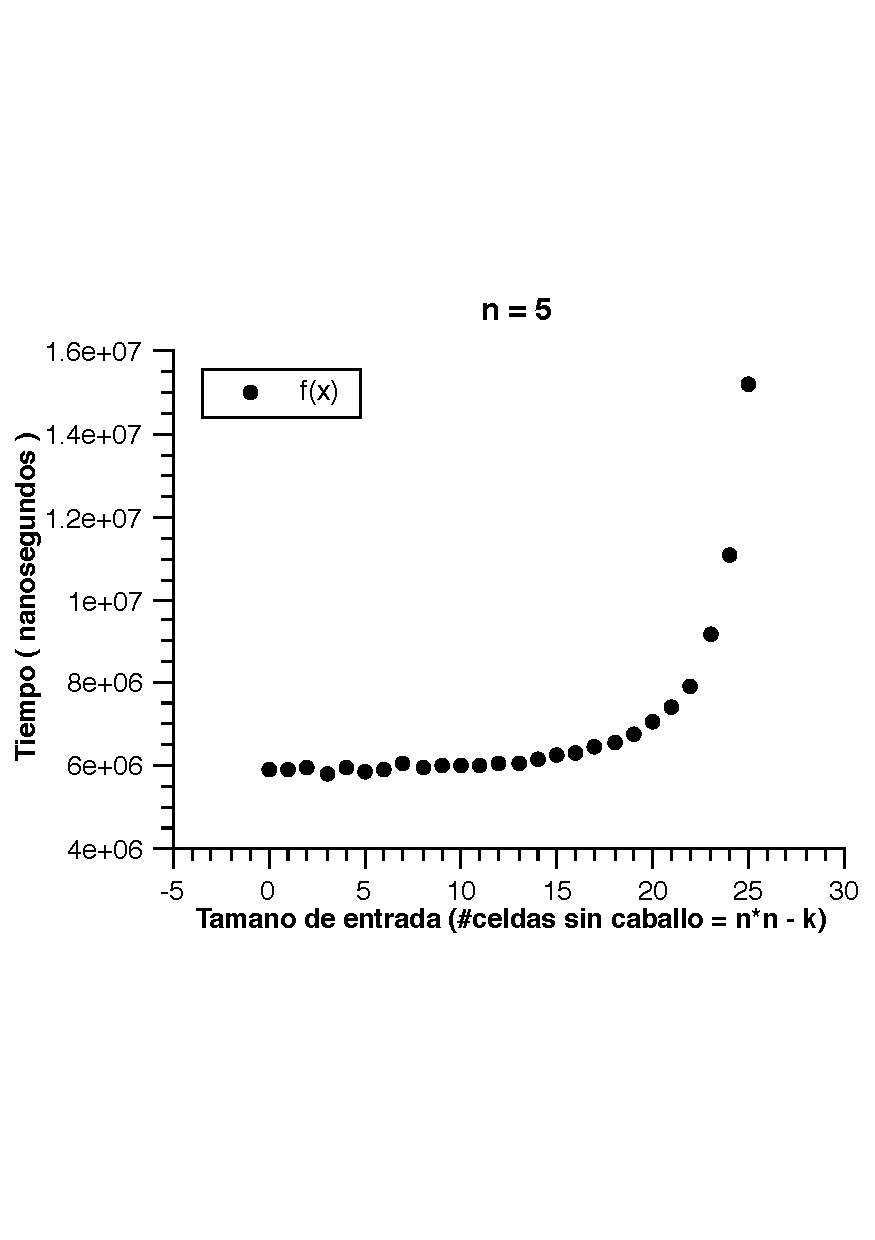
\includegraphics[width=\textwidth]{imagenes/grafico3-n-5-norm.pdf}
                \caption{Tiempos sin procesar}
        \end{subfigure}%
        ~ %add desired spacing between images, e. g. ~, \quad, \qquad, \hfill etc.
          %(or a blank line to force the subfigure onto a new line)
        \begin{subfigure}[b]{0.5\textwidth}
                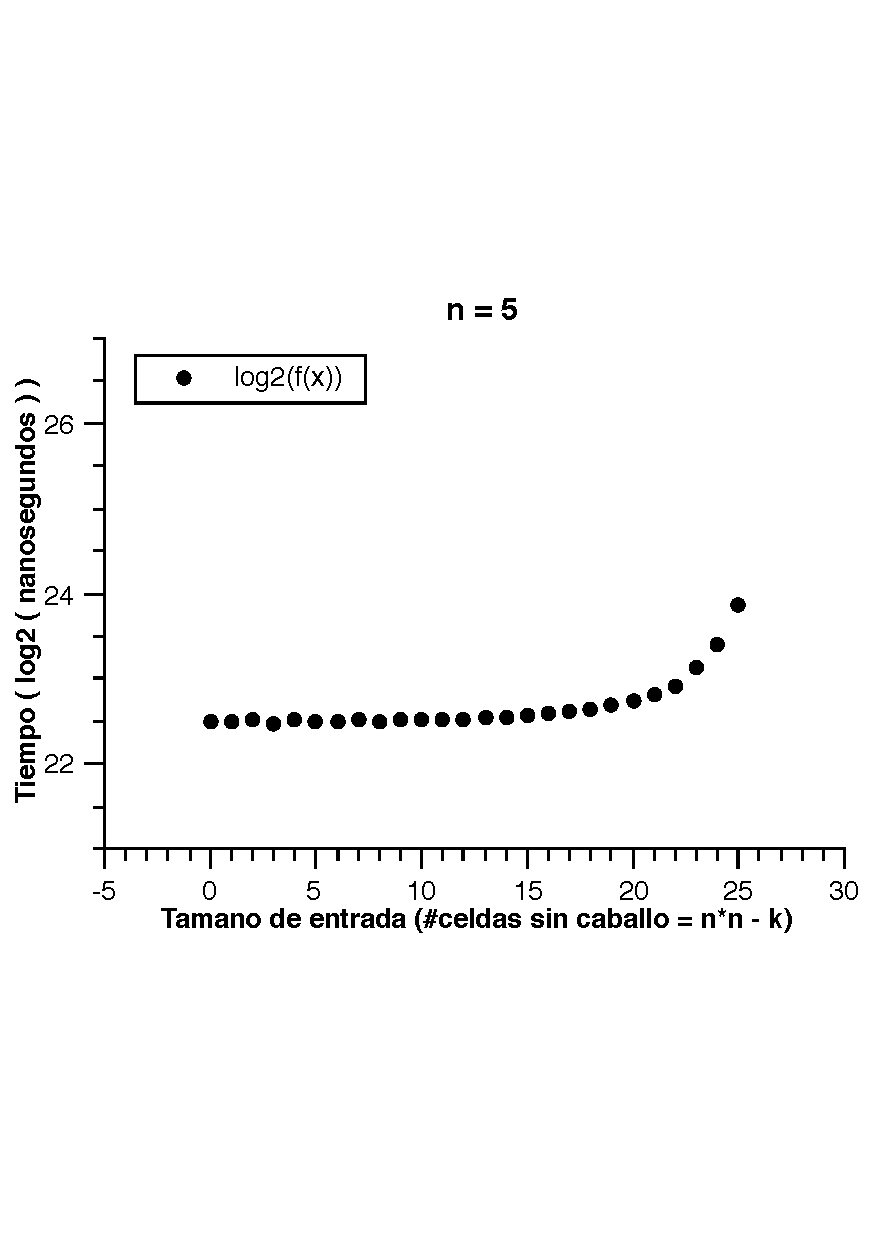
\includegraphics[width=\textwidth]{imagenes/grafico3-n-5-log.pdf}
                \caption{Logaritmo a la figura (a)}
        \end{subfigure}
        
        \begin{subfigure}[b]{0.5\textwidth}
                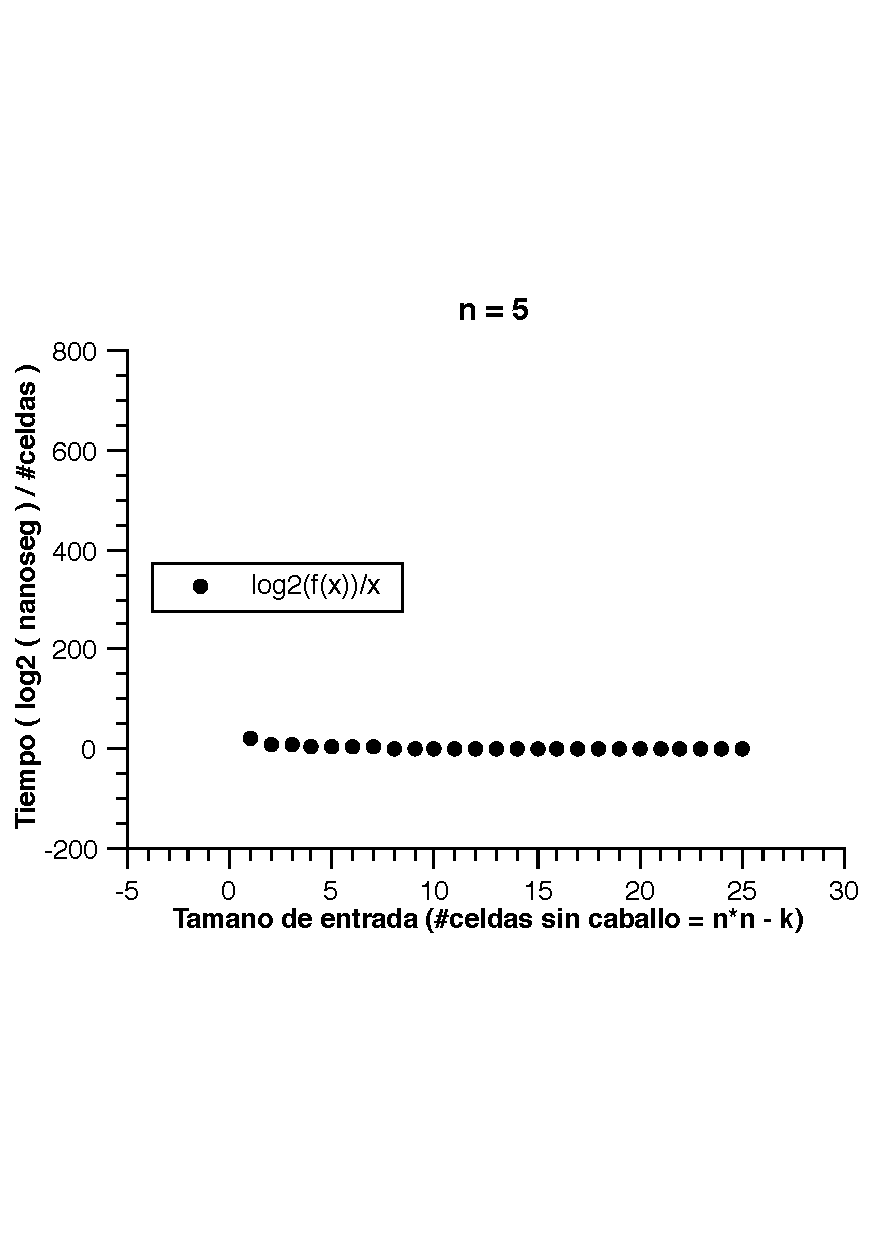
\includegraphics[width=\textwidth]{imagenes/grafico3-n-5-div-log.pdf}
                \caption{Dividiendo por x la figura (b)}
        \end{subfigure}
        \caption{Gráficos para $n=5$ sin podas G ni S}
\end{figure}

\begin{figure}[H]
        \centering
        \begin{subfigure}[b]{0.5\textwidth}
                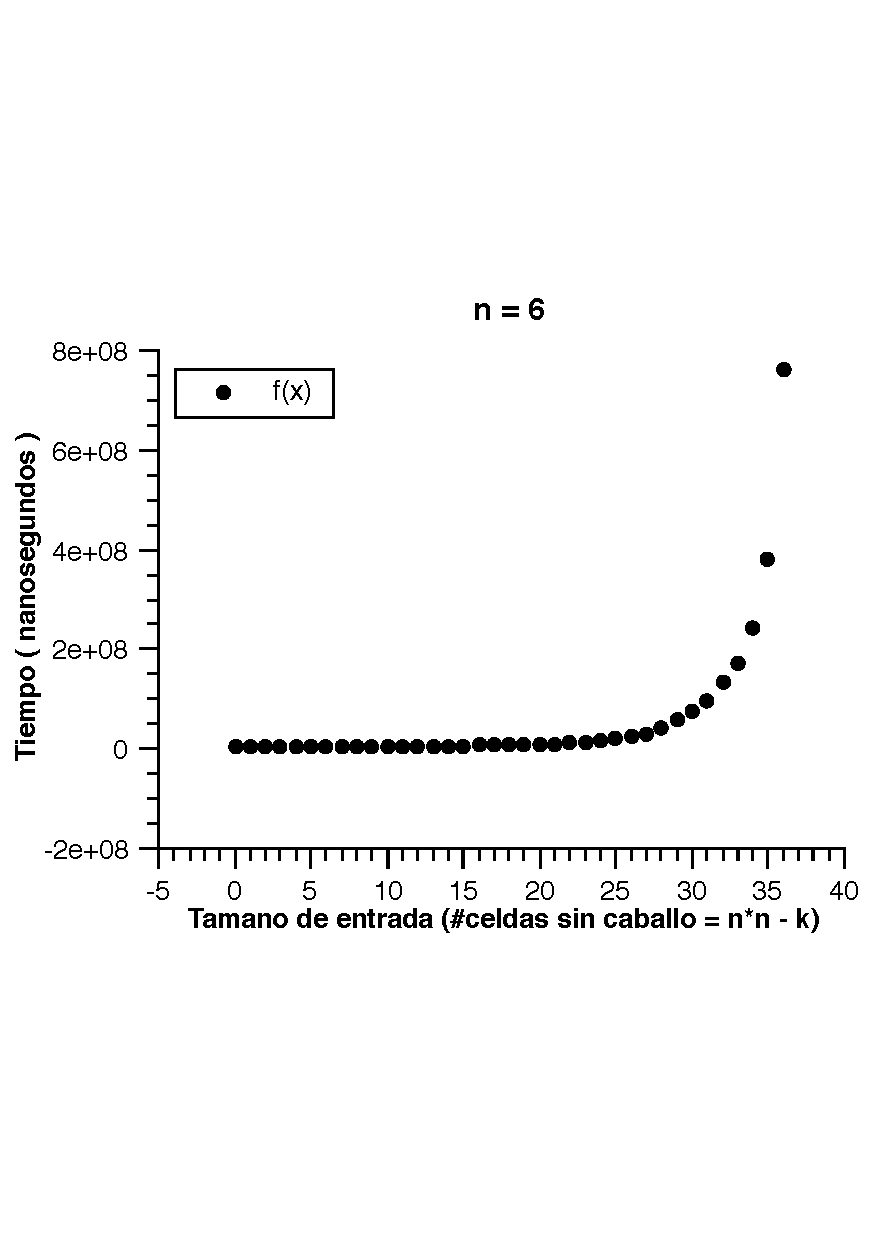
\includegraphics[width=\textwidth]{imagenes/grafico3-n-6-norm.pdf}
                \caption{Tiempos sin procesar}
        \end{subfigure}%
        ~ %add desired spacing between images, e. g. ~, \quad, \qquad, \hfill etc.
          %(or a blank line to force the subfigure onto a new line)
        \begin{subfigure}[b]{0.5\textwidth}
                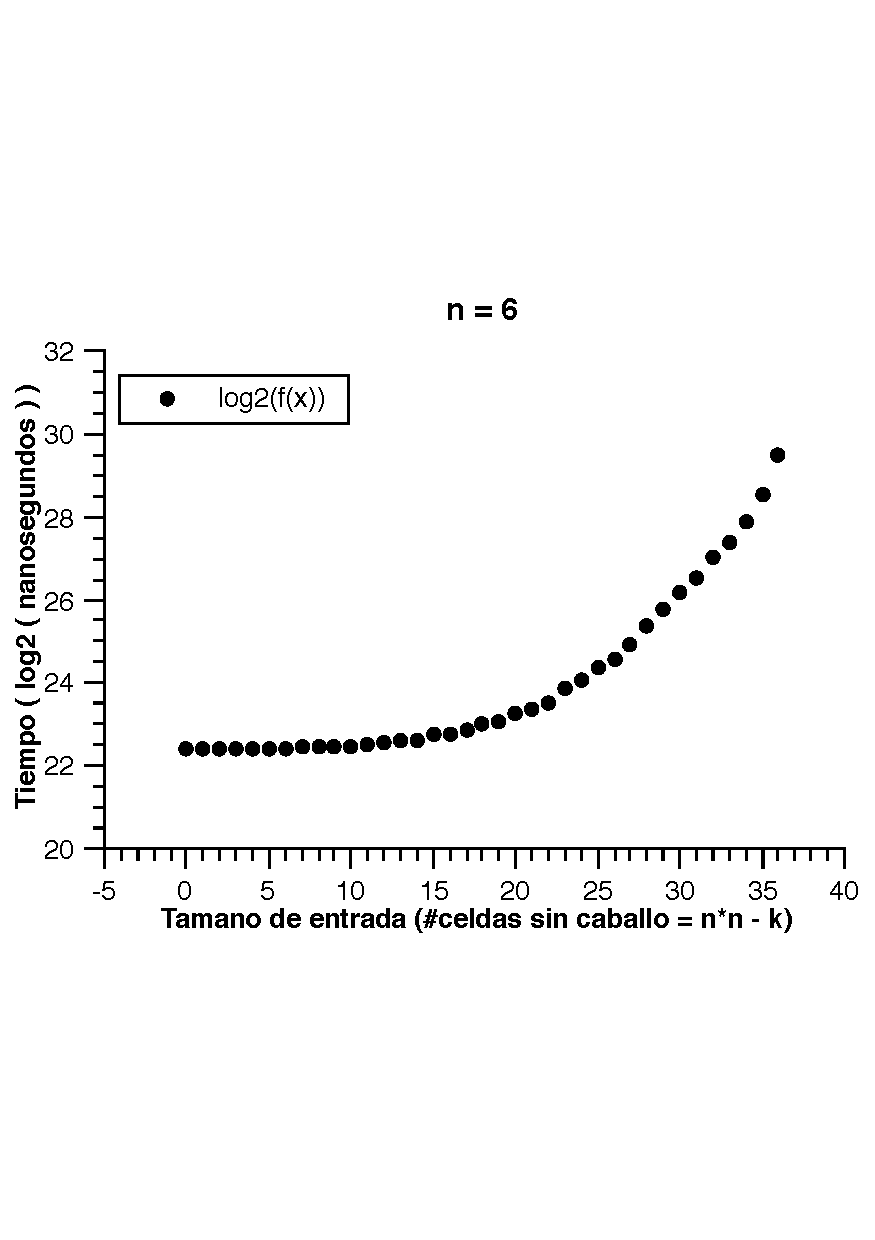
\includegraphics[width=\textwidth]{imagenes/grafico3-n-6-log.pdf}
                \caption{Logaritmo a la figura (a)}
        \end{subfigure}
        
        \begin{subfigure}[b]{0.5\textwidth}
                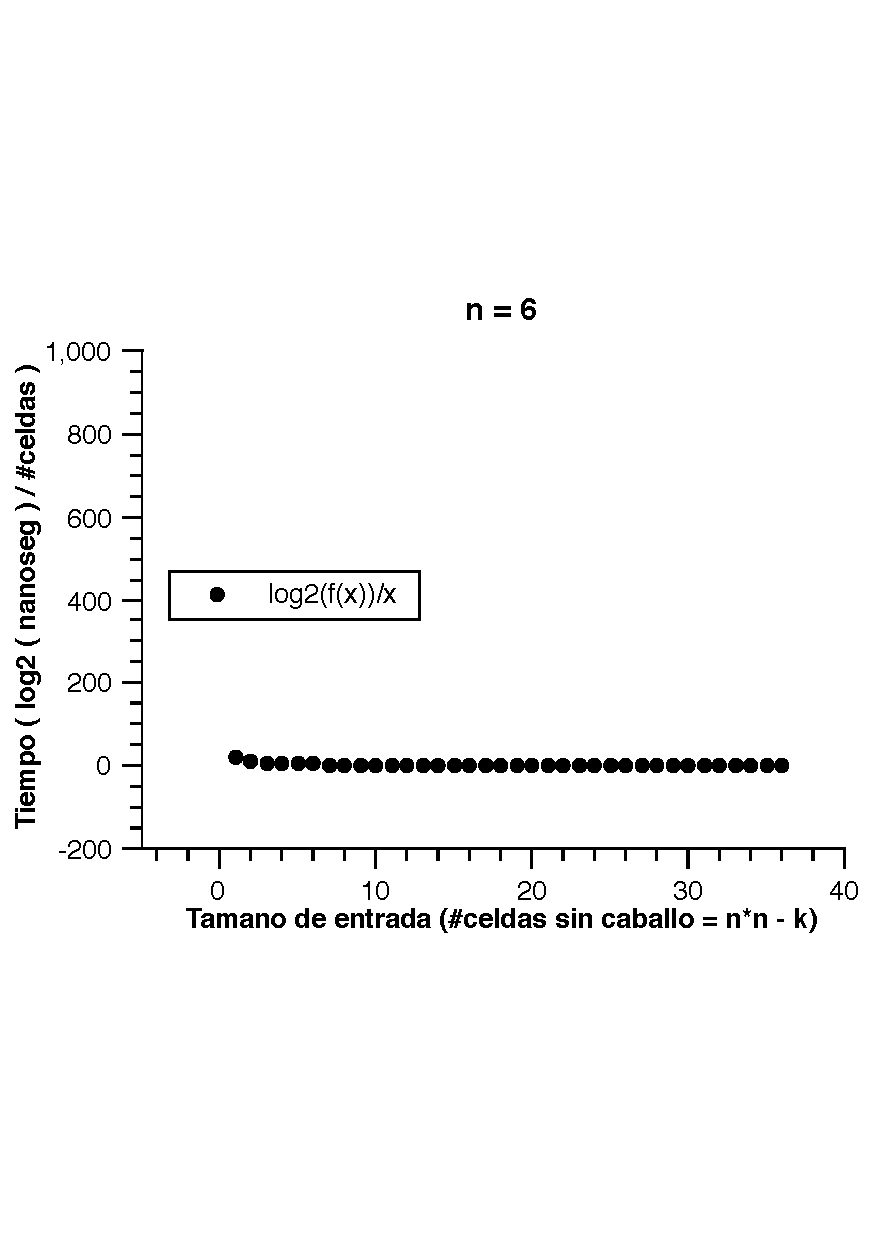
\includegraphics[width=\textwidth]{imagenes/grafico3-n-6-div-log.pdf}
                \caption{Dividiendo por x la figura (b)}
        \end{subfigure}
        \caption{Gráficos para $n=6$ sin podas G ni S}
\end{figure}

\begin{figure}[H]
        \centering
        \begin{subfigure}[b]{0.5\textwidth}
                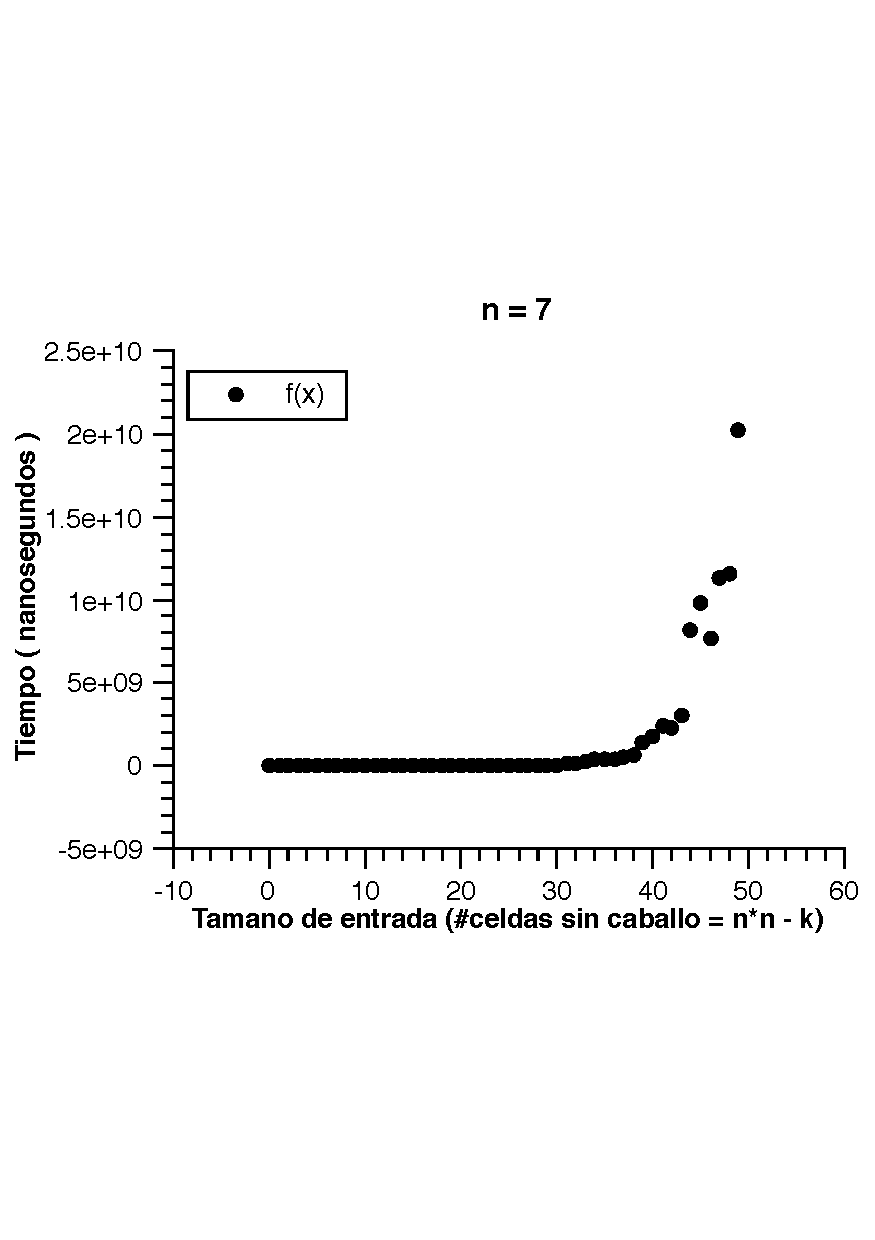
\includegraphics[width=\textwidth]{imagenes/grafico3-n-7-norm.pdf}
                \caption{Tiempos sin procesar}
        \end{subfigure}%
        ~ %add desired spacing between images, e. g. ~, \quad, \qquad, \hfill etc.
          %(or a blank line to force the subfigure onto a new line)
        \begin{subfigure}[b]{0.5\textwidth}
                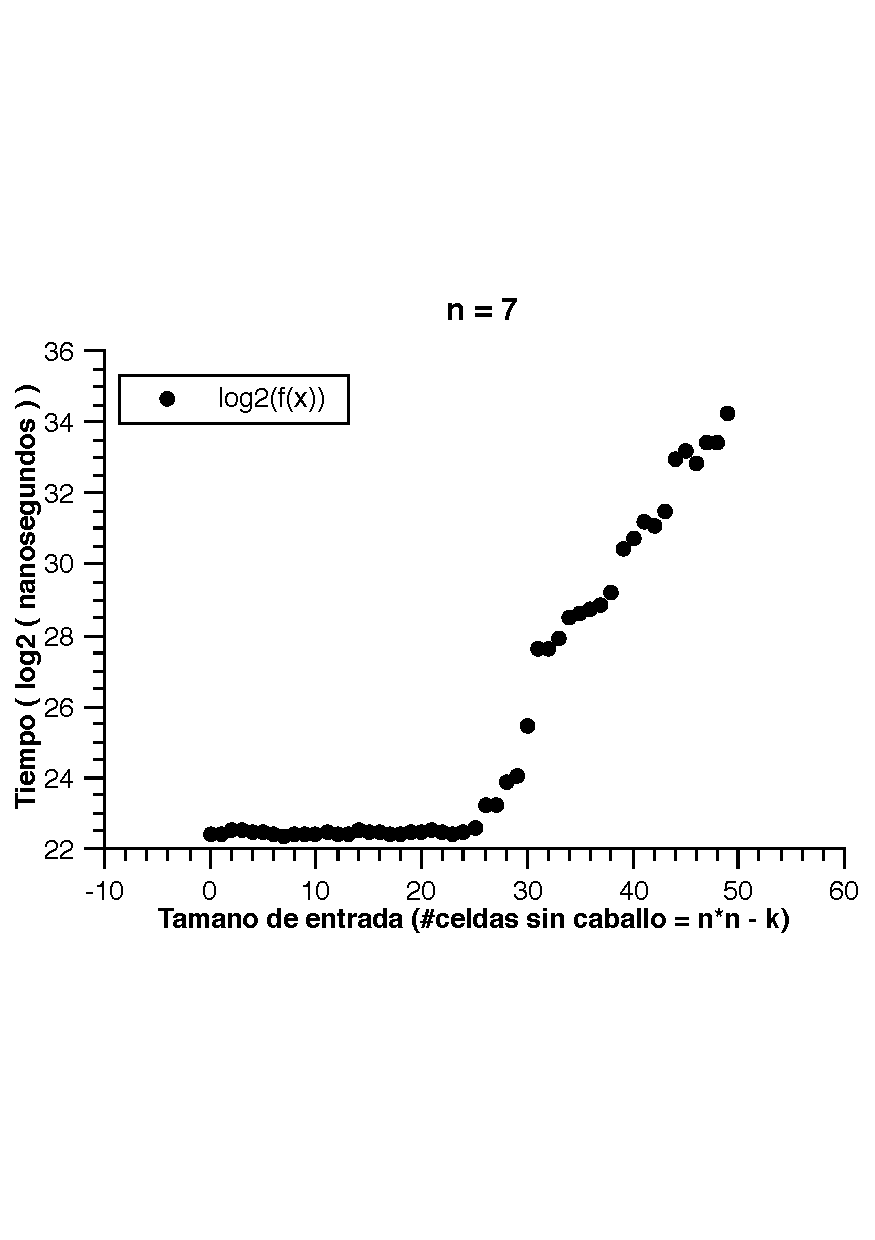
\includegraphics[width=\textwidth]{imagenes/grafico3-n-7-log.pdf}
                \caption{Logaritmo a la figura (a)}
        \end{subfigure}
        
        \begin{subfigure}[b]{0.5\textwidth}
                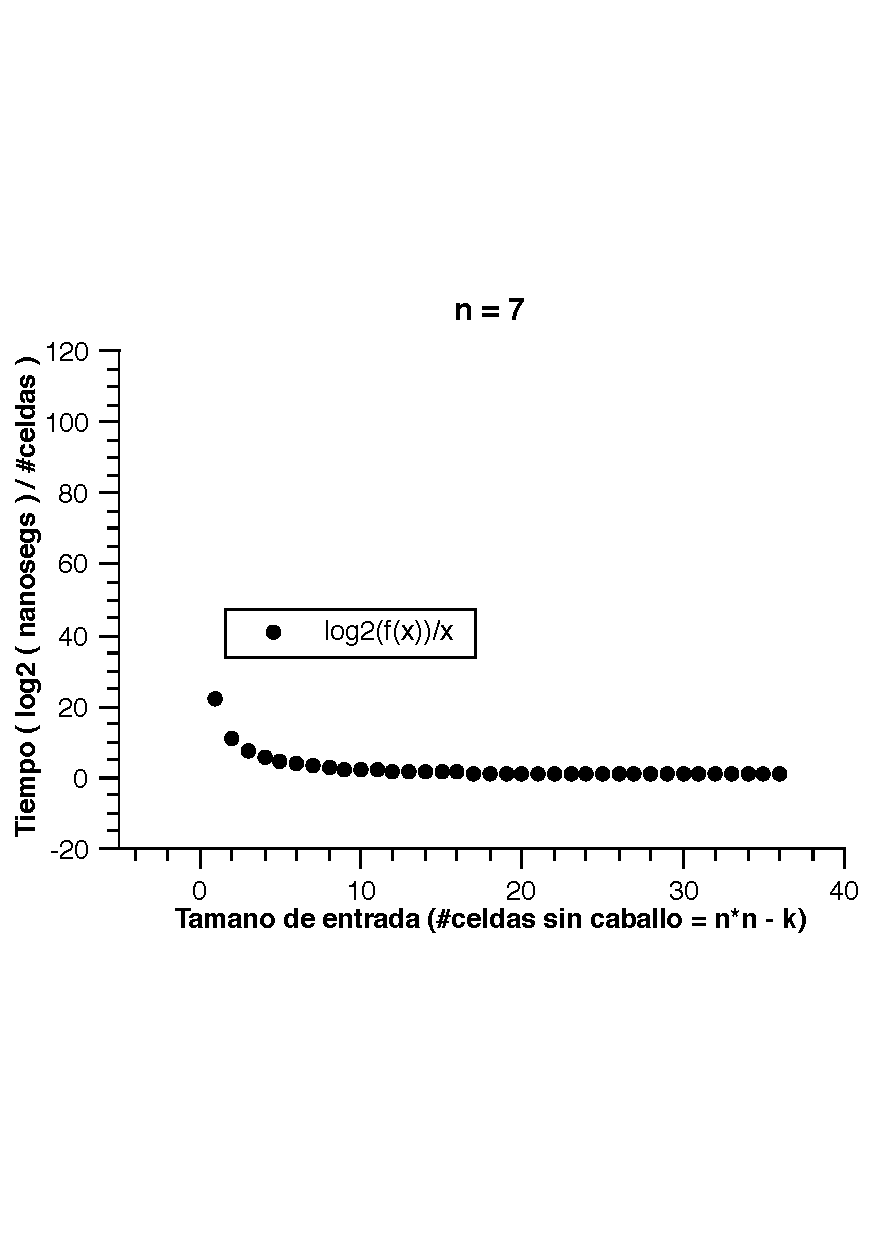
\includegraphics[width=\textwidth]{imagenes/grafico3-n-7-div-log.pdf}
                \caption{Dividiendo por x la figura (b)}
        \end{subfigure}
        \caption{Gráficos para $n=7$ sin podas G ni S}
\end{figure}

Con sus respectivas tablas en el Anexo \ref{sec:tablas-ej3}. \textit{Nota: se quitaron las podas G y S para facilitar el análisis del gráfico.}

Como podemos ver de los gráficos 1, 2 y 3 y sus respectivas tablas, al aplicarles logaritmo y dividirlos por x, todos tienden a un número constante entre cero y uno (para más detalles, se puede ver la tabla de valores en el anexo). Entonces nuestro algoritmo tendría complejidad $\mathcal{O}(c*2^{n^2 - k})$, donde $c$ es la constante a la cual converge el gráfico. Por lo tanto concluimos que los gráficos se condicen con nuestra predicción de complejidad.

\subsubsection{Experimentación con instancias particulares}

La experimentación con instancias particulares se realizó dejando el $k$ fijo en cero y variando el $n$ de 1 a 8:

\begin{figure}[H]
        \centering
        \begin{subfigure}[b]{0.5\textwidth}
                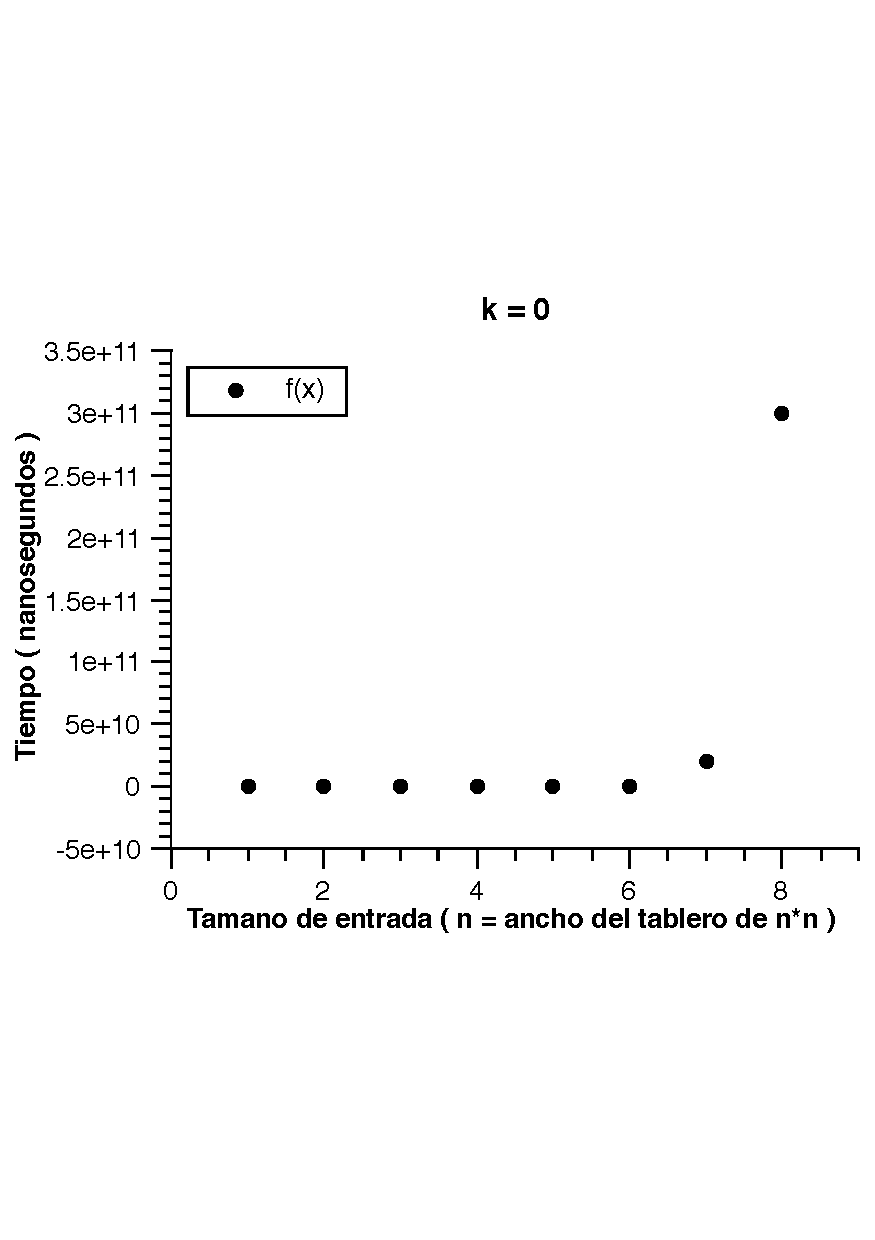
\includegraphics[width=\textwidth]{imagenes/grafico3-k-0-norm.pdf}
                \caption{Tiempos sin procesar}
        \end{subfigure}%
        ~ %add desired spacing between images, e. g. ~, \quad, \qquad, \hfill etc.
          %(or a blank line to force the subfigure onto a new line)
        \begin{subfigure}[b]{0.5\textwidth}
                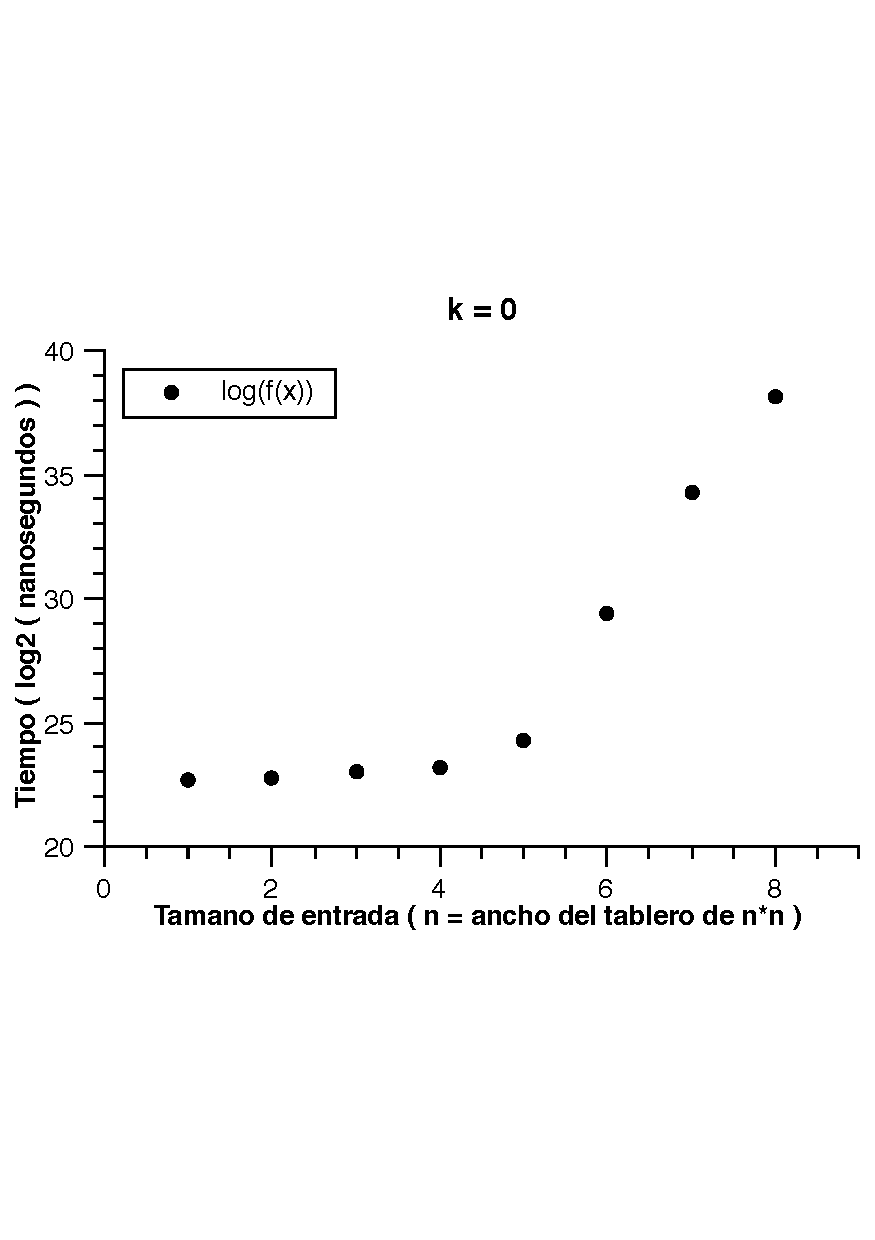
\includegraphics[width=\textwidth]{imagenes/grafico3-k-0-log.pdf}
                \caption{Logaritmo a la figura (a)}
        \end{subfigure}
        
        \begin{subfigure}[b]{0.5\textwidth}
                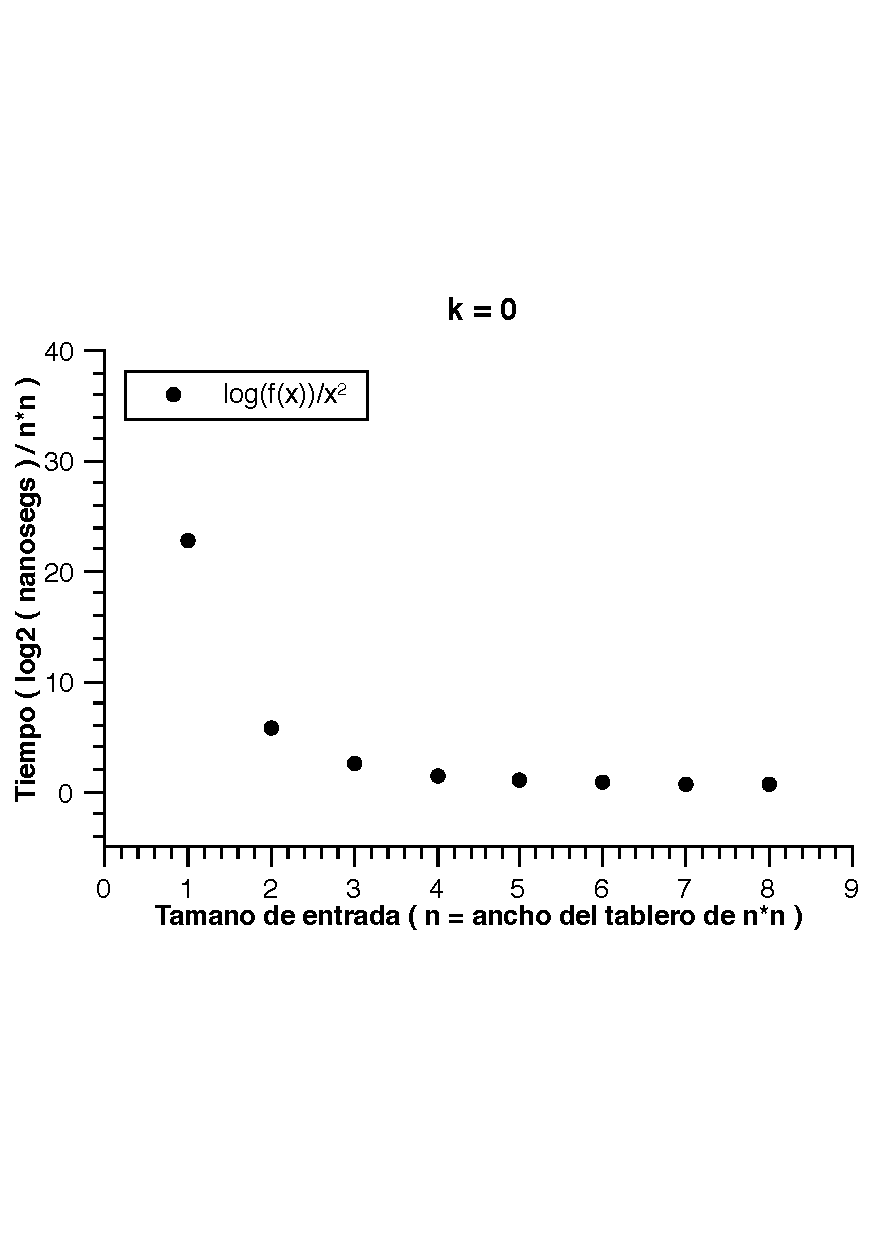
\includegraphics[width=\textwidth]{imagenes/grafico3-k-0-div-log.pdf}
                \caption{Dividiendo por x la figura (b)}
        \end{subfigure}
        \caption{Gráficos para $k=0$}
\end{figure}

Y su tabla también puede encontrarse en el Anexo \ref{sec:tablas-ej3}.

Para este experimento se utilizaron todas las podas detalladas anteriormente.
Se deprenden entonces los mismos resultados observados en los gráficos y tablas anteriores (el razonamiento es identico).

\subsubsection{Experimentación sin Podas}

Por último, se realizaron experimentaciones para comparar las mejoras aportadas por las podas:

\begin{figure}[H]
        \centering
        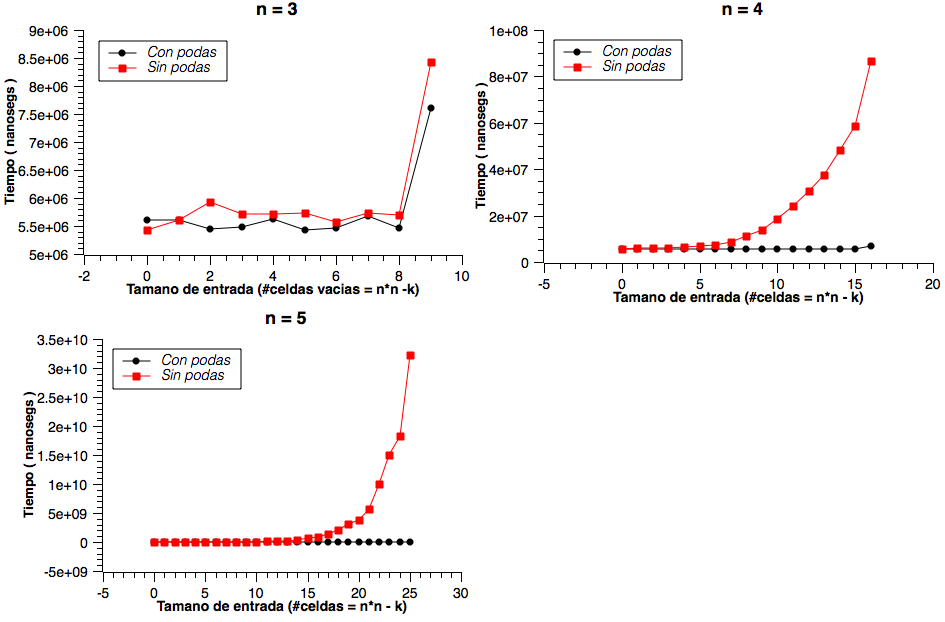
\includegraphics[width=\textwidth]{imagenes/grafico3-cmp-podas.png}
        \caption{Gráficos para $n=3,\ 4\ y\ 5$ comparando con podas vs. sin podas}
\end{figure}

\textit{Nota: el grafico sin podas sigue teniendo las podas B y C, ya que estás son las que hacen que el algoritmo devuelva soluciones correctas y no incorrectas.}

Y su tabla también puede hallarse en el Anexo  \ref{sec:tablas-ej3}.


\newpage
\appendix
% \section{Tablas Ejercicio 1} \label{sec:tablas-ej1}
\subsection{Instancias Aleatorias}
\begin{table}[H]
\parbox{0.3\textwidth}{
  \begin{tabular}{| l | l | l |l |}
    \hline
    Tamano($n$) & Tiempo($t$) & $t / log(n)$ & $t / n*log(n)$ \\ \hline
   271	&	510	&	63,10	&	0,233	\\ \hline
330	&	598	&	71,48	&	0,217	\\ \hline
537	&	958	&	105,64	&	0,197	\\ \hline
614	&	1.058	&	114,23	&	0,186	\\ \hline
940	&	3.641	&	368,65	&	0,392	\\ \hline
1.748	&	4.912	&	456,02	&	0,261	\\ \hline
2.086	&	3.595	&	326,03	&	0,156	\\ \hline
2.345	&	3.955	&	353,27	&	0,151	\\ \hline
2.390	&	4.137	&	368,62	&	0,154	\\ \hline
2.893	&	4.910	&	427,02	&	0,148	\\ \hline
3.451	&	5.865	&	499,03	&	0,145	\\ \hline
3.453	&	7.197	&	612,32	&	0,177	\\ \hline
3.585	&	6.957	&	589,19	&	0,164	\\ \hline
3.652	&	10.326	&	872,54	&	0,239	\\ \hline
4.098	&	14.579	&	1.214,85	&	0,296	\\ \hline
4.159	&	10.427	&	867,33	&	0,209	\\ \hline
4.168	&	9.553	&	794,42	&	0,191	\\ \hline
4.713	&	8.137	&	666,83	&	0,141	\\ \hline
4.786	&	12.340	&	1.009,44	&	0,211	\\ \hline
4.849	&	12.842	&	1.048,89	&	0,216	\\ \hline
5.128	&	8.800	&	714,04	&	0,139	\\ \hline
5.430	&	13.024	&	1.049,75	&	0,193	\\ \hline
5.760	&	13.980	&	1.119,13	&	0,194	\\ \hline
6.031	&	13.581	&	1.081,45	&	0,179	\\ \hline
6.084	&	11.125	&	884,99	&	0,145	\\ \hline
6.145	&	14.428	&	1.146,43	&	0,187	\\ \hline
6.233	&	15.134	&	1.200,57	&	0,193	\\ \hline
6.275	&	10.747	&	851,90	&	0,136	\\ \hline
6.411	&	10.953	&	866,10	&	0,135	\\ \hline
7.333	&	12.593	&	980,75	&	0,134	\\ \hline
7.653	&	13.165	&	1.020,40	&	0,133	\\ \hline
7.925	&	13.543	&	1.045,61	&	0,132	\\ \hline
7.958	&	15.081	&	1.163,82	&	0,146	\\ \hline
8.062	&	13.838	&	1.066,35	&	0,132	\\ \hline
8.122	&	20.788	&	1.600,60	&	0,197	\\ \hline
8.187	&	15.871	&	1.220,93	&	0,149	\\ \hline
8.213	&	14.799	&	1.138,06	&	0,139	\\ \hline
8.466	&	21.715	&	1.664,31	&	0,197	\\ \hline
8.504	&	19.453	&	1.490,20	&	0,175	\\ \hline
8.586	&	23.741	&	1.816,76	&	0,212	\\ \hline
8.955	&	17.885	&	1.362,31	&	0,152	\\ \hline
8.996	&	20.332	&	1.547,92	&	0,172	\\ \hline
  \end{tabular}
   \caption*{Tabla 1/12}
}
\end{table}
\begin{table}[H]
\parbox{0.3\textwidth}{
  \begin{tabular}{| l | l | l |l |}
    \hline
    Tamano($n$) & Tiempo($t$) & $t / log(n)$ & $t / n*log(n)$ \\ \hline
9.047	&	20.220	&	1.538,44	&	0,170	\\ \hline
9.122	&	15.921	&	1.210,25	&	0,133	\\ \hline
9.299	&	16.616	&	1.260,42	&	0,136	\\ \hline
9.478	&	17.568	&	1.329,86	&	0,140	\\ \hline
9.780	&	17.630	&	1.330,00	&	0,136	\\ \hline
9.909	&	23.867	&	1.797,96	&	0,181	\\ \hline
10.329	&	19.373	&	1.452,86	&	0,141	\\ \hline
10.456	&	19.555	&	1.464,57	&	0,140	\\ \hline
10.545	&	19.838	&	1.484,41	&	0,141	\\ \hline
10.610	&	26.497	&	1.981,36	&	0,187	\\ \hline
10.662	&	18.424	&	1.376,96	&	0,129	\\ \hline
10.830	&	25.672	&	1.915,43	&	0,177	\\ \hline
10.910	&	22.681	&	1.690,93	&	0,155	\\ \hline
10.946	&	25.839	&	1.925,68	&	0,176	\\ \hline
11.007	&	22.085	&	1.644,93	&	0,149	\\ \hline
11.120	&	21.517	&	1.600,86	&	0,144	\\ \hline
11.225	&	19.340	&	1.437,44	&	0,128	\\ \hline
11.312	&	24.947	&	1.852,65	&	0,164	\\ \hline
11.368	&	19.643	&	1.457,99	&	0,128	\\ \hline
11.897	&	21.330	&	1.575,53	&	0,132	\\ \hline
12.049	&	26.937	&	1.987,00	&	0,165	\\ \hline
12.281	&	22.794	&	1.677,99	&	0,137	\\ \hline
12.329	&	22.052	&	1.622,69	&	0,132	\\ \hline
12.645	&	23.881	&	1.752,57	&	0,139	\\ \hline
12.721	&	22.866	&	1.677,02	&	0,132	\\ \hline
12.868	&	26.964	&	1.975,17	&	0,153	\\ \hline
13.006	&	23.309	&	1.705,51	&	0,131	\\ \hline
13.010	&	25.779	&	1.886,18	&	0,145	\\ \hline
13.017	&	28.668	&	2.097,44	&	0,161	\\ \hline
13.048	&	24.299	&	1.777,34	&	0,136	\\ \hline
13.107	&	22.913	&	1.675,17	&	0,128	\\ \hline
13.607	&	25.396	&	1.849,39	&	0,136	\\ \hline
13.648	&	25.051	&	1.823,69	&	0,134	\\ \hline
13.837	&	23.864	&	1.734,78	&	0,125	\\ \hline
14.066	&	29.308	&	2.126,86	&	0,151	\\ \hline
14.081	&	27.346	&	1.984,26	&	0,141	\\ \hline
14.114	&	29.329	&	2.127,63	&	0,151	\\ \hline
14.273	&	24.974	&	1.809,58	&	0,127	\\ \hline
14.540	&	25.952	&	1.876,81	&	0,129	\\ \hline
14.774	&	27.302	&	1.971,15	&	0,133	\\ \hline
14.911	&	27.463	&	1.980,87	&	0,133	\\ \hline
15.981	&	32.518	&	2.328,69	&	0,146	\\ \hline
  \end{tabular}
  \caption*{Tabla 2/12}
}
\end{table}
\begin{table}[H]
\parbox{0.3\textwidth}{
  \begin{tabular}{| l | l | l |l |}
    \hline
    Tamano($n$) & Tiempo($t$) & $t / log(n)$ & $t / n*log(n)$ \\ \hline
16.119	&	33.946	&	2.428,80	&	0,151	\\ \hline
16.749	&	29.334	&	2.090,54	&	0,125	\\ \hline
16.929	&	32.238	&	2.294,98	&	0,136	\\ \hline
16.975	&	30.603	&	2.177,98	&	0,128	\\ \hline
17.253	&	30.130	&	2.140,74	&	0,124	\\ \hline
17.732	&	35.128	&	2.488,86	&	0,140	\\ \hline
17.815	&	31.067	&	2.200,09	&	0,123	\\ \hline
17.992	&	33.129	&	2.343,75	&	0,130	\\ \hline
18.083	&	37.809	&	2.673,46	&	0,148	\\ \hline
18.476	&	33.828	&	2.386,73	&	0,129	\\ \hline
18.497	&	32.259	&	2.275,77	&	0,123	\\ \hline
19.046	&	38.834	&	2.731,48	&	0,143	\\ \hline
19.330	&	34.218	&	2.403,19	&	0,124	\\ \hline
19.364	&	35.589	&	2.499,04	&	0,129	\\ \hline
19.749	&	34.663	&	2.429,17	&	0,123	\\ \hline
20.165	&	36.214	&	2.532,52	&	0,126	\\ \hline
20.346	&	37.056	&	2.589,07	&	0,127	\\ \hline
20.500	&	41.954	&	2.929,07	&	0,143	\\ \hline
21.328	&	41.098	&	2.857,91	&	0,134	\\ \hline
21.521	&	39.825	&	2.766,88	&	0,129	\\ \hline
23.231	&	40.624	&	2.800,93	&	0,121	\\ \hline
23.815	&	43.206	&	2.971,61	&	0,125	\\ \hline
23.880	&	45.530	&	3.130,60	&	0,131	\\ \hline
24.176	&	42.234	&	2.900,43	&	0,120	\\ \hline
24.359	&	44.020	&	3.020,83	&	0,124	\\ \hline
24.364	&	44.351	&	3.043,48	&	0,125	\\ \hline
24.501	&	42.944	&	2.945,29	&	0,120	\\ \hline
24.607	&	50.331	&	3.450,45	&	0,140	\\ \hline
24.645	&	44.789	&	3.070,05	&	0,125	\\ \hline
24.653	&	50.141	&	3.436,79	&	0,139	\\ \hline
24.828	&	43.785	&	2.999,04	&	0,121	\\ \hline
24.843	&	46.056	&	3.154,40	&	0,127	\\ \hline
24.862	&	49.145	&	3.365,71	&	0,135	\\ \hline
24.920	&	45.598	&	3.122,08	&	0,125	\\ \hline
24.925	&	44.659	&	3.057,72	&	0,123	\\ \hline
25.148	&	51.010	&	3.489,50	&	0,139	\\ \hline
25.622	&	46.791	&	3.194,99	&	0,125	\\ \hline
25.645	&	45.785	&	3.126,03	&	0,122	\\ \hline
25.988	&	45.731	&	3.118,26	&	0,120	\\ \hline
26.532	&	53.420	&	3.635,14	&	0,137	\\ \hline
26.710	&	53.263	&	3.622,08	&	0,136	\\ \hline
26.864	&	47.112	&	3.201,98	&	0,119	\\ \hline
  \end{tabular}
  \caption*{Tabla 3/12}
}
\end{table}
\begin{table}[H]
\parbox{0.3\textwidth}{
  \begin{tabular}{| l | l | l |l |}
    \hline
    Tamano($n$) & Tiempo($t$) & $t / log(n)$ & $t / n*log(n)$ \\ \hline
26.923	&	53.728	&	3.650,86	&	0,136	\\ \hline
26.936	&	48.875	&	3.320,93	&	0,123	\\ \hline
27.076	&	53.090	&	3.605,50	&	0,133	\\ \hline
27.151	&	49.036	&	3.329,28	&	0,123	\\ \hline
27.312	&	48.309	&	3.278,02	&	0,120	\\ \hline
27.460	&	51.835	&	3.515,42	&	0,128	\\ \hline
27.873	&	57.937	&	3.923,52	&	0,141	\\ \hline
27.938	&	50.667	&	3.430,41	&	0,123	\\ \hline
28.535	&	51.057	&	3.449,69	&	0,121	\\ \hline
28.958	&	58.634	&	3.955,96	&	0,137	\\ \hline
29.344	&	55.209	&	3.720,09	&	0,127	\\ \hline
29.381	&	58.788	&	3.960,76	&	0,135	\\ \hline
29.765	&	53.536	&	3.602,37	&	0,121	\\ \hline
29.803	&	58.879	&	3.961,40	&	0,133	\\ \hline
30.029	&	53.011	&	3.563,99	&	0,119	\\ \hline
30.239	&	54.537	&	3.664,11	&	0,121	\\ \hline
30.380	&	60.550	&	4.066,26	&	0,134	\\ \hline
30.682	&	57.935	&	3.886,92	&	0,127	\\ \hline
30.982	&	59.582	&	3.993,66	&	0,129	\\ \hline
31.176	&	55.229	&	3.699,66	&	0,119	\\ \hline
31.186	&	62.837	&	4.209,17	&	0,135	\\ \hline
31.232	&	61.880	&	4.144,47	&	0,133	\\ \hline
31.511	&	56.705	&	3.794,61	&	0,120	\\ \hline
31.620	&	57.098	&	3.819,63	&	0,121	\\ \hline
32.208	&	57.004	&	3.806,58	&	0,118	\\ \hline
32.223	&	57.503	&	3.839,73	&	0,119	\\ \hline
32.373	&	63.551	&	4.241,68	&	0,131	\\ \hline
32.951	&	60.271	&	4.015,92	&	0,122	\\ \hline
33.014	&	63.065	&	4.201,31	&	0,127	\\ \hline
33.034	&	60.465	&	4.027,87	&	0,122	\\ \hline
33.076	&	59.328	&	3.951,64	&	0,119	\\ \hline
33.882	&	63.522	&	4.221,23	&	0,125	\\ \hline
34.261	&	62.812	&	4.169,60	&	0,122	\\ \hline
34.552	&	63.117	&	4.186,45	&	0,121	\\ \hline
34.575	&	61.668	&	4.090,08	&	0,118	\\ \hline
34.710	&	62.404	&	4.137,36	&	0,119	\\ \hline
34.877	&	62.256	&	4.125,65	&	0,118	\\ \hline
35.054	&	62.130	&	4.115,31	&	0,117	\\ \hline
35.278	&	66.797	&	4.421,74	&	0,125	\\ \hline
35.435	&	68.038	&	4.501,99	&	0,127	\\ \hline
35.499	&	62.881	&	4.160,04	&	0,117	\\ \hline
35.645	&	65.010	&	4.299,20	&	0,121	\\ \hline
  \end{tabular}
  \caption*{Tabla 4/12}
}
\end{table}
\begin{table}[H]
\parbox{0.3\textwidth}{
  \begin{tabular}{| l | l | l |l |}
    \hline
    Tamano($n$) & Tiempo($t$) & $t / log(n)$ & $t / n*log(n)$ \\ \hline
35.744	&	63.172	&	4.176,55	&	0,117	\\ \hline
35.819	&	63.473	&	4.195,61	&	0,117	\\ \hline
35.834	&	64.779	&	4.281,76	&	0,119	\\ \hline
36.024	&	70.654	&	4.667,74	&	0,130	\\ \hline
36.161	&	65.797	&	4.345,29	&	0,120	\\ \hline
36.375	&	67.246	&	4.438,49	&	0,122	\\ \hline
36.497	&	68.334	&	4.508,86	&	0,124	\\ \hline
36.591	&	68.376	&	4.510,53	&	0,123	\\ \hline
36.715	&	72.381	&	4.773,19	&	0,130	\\ \hline
36.913	&	68.572	&	4.519,69	&	0,122	\\ \hline
37.002	&	65.440	&	4.312,27	&	0,117	\\ \hline
37.117	&	65.674	&	4.326,41	&	0,117	\\ \hline
37.652	&	66.864	&	4.398,82	&	0,117	\\ \hline
37.783	&	68.381	&	4.497,14	&	0,119	\\ \hline
37.811	&	68.751	&	4.521,15	&	0,120	\\ \hline
38.906	&	74.607	&	4.893,00	&	0,126	\\ \hline
39.133	&	70.444	&	4.617,43	&	0,118	\\ \hline
39.824	&	70.782	&	4.631,92	&	0,116	\\ \hline
40.369	&	72.406	&	4.732,12	&	0,117	\\ \hline
41.048	&	74.943	&	4.890,24	&	0,119	\\ \hline
41.223	&	79.331	&	5.174,49	&	0,126	\\ \hline
41.278	&	82.620	&	5.388,35	&	0,131	\\ \hline
41.413	&	77.273	&	5.038,08	&	0,122	\\ \hline
41.897	&	79.133	&	5.153,71	&	0,123	\\ \hline
42.182	&	75.115	&	4.888,92	&	0,116	\\ \hline
42.230	&	75.125	&	4.889,05	&	0,116	\\ \hline
43.173	&	79.527	&	5.164,81	&	0,120	\\ \hline
43.346	&	82.846	&	5.378,35	&	0,124	\\ \hline
43.479	&	77.259	&	5.014,20	&	0,115	\\ \hline
43.586	&	78.765	&	5.110,77	&	0,117	\\ \hline
43.831	&	78.321	&	5.079,29	&	0,116	\\ \hline
43.945	&	83.414	&	5.408,27	&	0,123	\\ \hline
44.074	&	79.874	&	5.177,33	&	0,117	\\ \hline
44.290	&	83.899	&	5.435,74	&	0,123	\\ \hline
44.478	&	82.785	&	5.361,44	&	0,121	\\ \hline
44.623	&	86.095	&	5.574,12	&	0,125	\\ \hline
44.733	&	80.572	&	5.215,34	&	0,117	\\ \hline
44.772	&	79.750	&	5.161,71	&	0,115	\\ \hline
44.893	&	81.290	&	5.260,06	&	0,117	\\ \hline
45.129	&	85.631	&	5.538,24	&	0,123	\\ \hline
45.216	&	80.127	&	5.181,34	&	0,115	\\ \hline
45.579	&	82.356	&	5.321,50	&	0,117	\\ \hline
  \end{tabular}
  \caption*{Tabla 5/12}
}
\end{table}
\begin{table}[H]
\parbox{0.3\textwidth}{
  \begin{tabular}{| l | l | l |l |}
    \hline
    Tamano($n$) & Tiempo($t$) & $t / log(n)$ & $t / n*log(n)$ \\ \hline
45.939	&	86.254	&	5.569,29	&	0,121	\\ \hline
46.141	&	85.702	&	5.531,39	&	0,120	\\ \hline
46.174	&	81.927	&	5.287,39	&	0,115	\\ \hline
46.191	&	82.500	&	5.324,19	&	0,115	\\ \hline
46.775	&	88.359	&	5.695,64	&	0,122	\\ \hline
46.786	&	90.141	&	5.810,38	&	0,124	\\ \hline
46.827	&	83.318	&	5.370,14	&	0,115	\\ \hline
47.087	&	85.777	&	5.525,79	&	0,117	\\ \hline
47.181	&	84.236	&	5.425,51	&	0,115	\\ \hline
47.643	&	85.109	&	5.476,78	&	0,115	\\ \hline
48.607	&	92.512	&	5.942,11	&	0,122	\\ \hline
48.778	&	91.000	&	5.843,09	&	0,120	\\ \hline
48.817	&	90.156	&	5.788,47	&	0,119	\\ \hline
49.022	&	95.255	&	6.113,48	&	0,125	\\ \hline
49.291	&	95.035	&	6.096,27	&	0,124	\\ \hline
49.331	&	89.352	&	5.731,29	&	0,116	\\ \hline
49.457	&	88.559	&	5.679,08	&	0,115	\\ \hline
49.731	&	95.624	&	6.129,01	&	0,123	\\ \hline
50.346	&	93.461	&	5.983,58	&	0,119	\\ \hline
50.678	&	91.898	&	5.879,94	&	0,116	\\ \hline
50.720	&	97.807	&	6.257,54	&	0,123	\\ \hline
50.726	&	91.500	&	5.853,96	&	0,115	\\ \hline
50.901	&	92.377	&	5.908,19	&	0,116	\\ \hline
50.973	&	97.156	&	6.213,04	&	0,122	\\ \hline
50.998	&	91.423	&	5.846,15	&	0,115	\\ \hline
51.527	&	92.518	&	5.910,54	&	0,115	\\ \hline
51.552	&	92.185	&	5.889,01	&	0,114	\\ \hline
51.592	&	93.698	&	5.985,23	&	0,116	\\ \hline
51.753	&	92.747	&	5.922,79	&	0,114	\\ \hline
51.862	&	96.482	&	6.160,11	&	0,119	\\ \hline
51.961	&	95.809	&	6.116,06	&	0,118	\\ \hline
51.973	&	99.384	&	6.344,14	&	0,122	\\ \hline
52.679	&	99.273	&	6.329,19	&	0,120	\\ \hline
52.936	&	95.239	&	6.069,29	&	0,115	\\ \hline
53.226	&	98.952	&	6.302,74	&	0,118	\\ \hline
53.431	&	96.597	&	6.150,56	&	0,115	\\ \hline
53.651	&	95.065	&	6.050,73	&	0,113	\\ \hline
53.823	&	97.920	&	6.230,62	&	0,116	\\ \hline
54.036	&	99.436	&	6.324,79	&	0,117	\\ \hline
54.389	&	104.644	&	6.652,08	&	0,122	\\ \hline
54.476	&	102.266	&	6.499,96	&	0,119	\\ \hline
54.496	&	100.051	&	6.358,96	&	0,117	\\ \hline
  \end{tabular}
  \caption*{Tabla 6/12}
}
\end{table}
\begin{table}[H]
\parbox{0.3\textwidth}{
  \begin{tabular}{| l | l | l |l |}
    \hline
    Tamano($n$) & Tiempo($t$) & $t / log(n)$ & $t / n*log(n)$ \\ \hline
54.730	&	98.581	&	6.263,07	&	0,114	\\ \hline
54.831	&	103.389	&	6.567,42	&	0,120	\\ \hline
54.896	&	98.051	&	6.227,67	&	0,113	\\ \hline
55.149	&	99.489	&	6.316,34	&	0,115	\\ \hline
55.156	&	98.769	&	6.270,56	&	0,114	\\ \hline
55.200	&	99.076	&	6.289,59	&	0,114	\\ \hline
55.223	&	104.374	&	6.625,67	&	0,120	\\ \hline
55.665	&	99.898	&	6.336,90	&	0,114	\\ \hline
55.808	&	99.759	&	6.326,60	&	0,113	\\ \hline
55.819	&	100.917	&	6.399,92	&	0,115	\\ \hline
56.020	&	102.179	&	6.477,83	&	0,116	\\ \hline
56.278	&	107.357	&	6.803,24	&	0,121	\\ \hline
56.294	&	100.954	&	6.397,31	&	0,114	\\ \hline
56.562	&	106.036	&	6.716,43	&	0,119	\\ \hline
56.681	&	105.722	&	6.695,26	&	0,118	\\ \hline
56.934	&	102.783	&	6.506,49	&	0,114	\\ \hline
57.077	&	103.891	&	6.575,12	&	0,115	\\ \hline
57.766	&	108.130	&	6.835,91	&	0,118	\\ \hline
57.985	&	108.136	&	6.833,93	&	0,118	\\ \hline
58.118	&	104.412	&	6.597,21	&	0,114	\\ \hline
58.395	&	110.914	&	7.005,00	&	0,120	\\ \hline
58.839	&	108.028	&	6.818,02	&	0,116	\\ \hline
59.029	&	107.995	&	6.813,94	&	0,115	\\ \hline
59.280	&	106.414	&	6.711,59	&	0,113	\\ \hline
59.371	&	106.083	&	6.689,78	&	0,113	\\ \hline
59.477	&	106.405	&	6.709,00	&	0,113	\\ \hline
59.879	&	109.720	&	6.913,78	&	0,115	\\ \hline
59.965	&	106.622	&	6.717,69	&	0,112	\\ \hline
60.163	&	112.806	&	7.105,18	&	0,118	\\ \hline
60.215	&	107.964	&	6.799,67	&	0,113	\\ \hline
60.564	&	116.298	&	7.320,71	&	0,121	\\ \hline
60.643	&	114.118	&	7.182,63	&	0,118	\\ \hline
60.713	&	110.216	&	6.936,31	&	0,114	\\ \hline
60.821	&	109.962	&	6.919,21	&	0,114	\\ \hline
60.859	&	110.060	&	6.924,98	&	0,114	\\ \hline
61.001	&	109.292	&	6.875,20	&	0,113	\\ \hline
61.346	&	114.264	&	7.184,30	&	0,117	\\ \hline
61.447	&	111.656	&	7.019,28	&	0,114	\\ \hline
61.673	&	109.557	&	6.885,03	&	0,112	\\ \hline
61.831	&	111.907	&	7.031,08	&	0,114	\\ \hline
61.916	&	110.945	&	6.969,77	&	0,113	\\ \hline
62.176	&	112.631	&	7.073,00	&	0,114	\\ \hline
  \end{tabular}
  \caption*{Tabla 7/12}
}
\end{table}
\begin{table}[H]
\parbox{0.3\textwidth}{
  \begin{tabular}{| l | l | l |l |}
    \hline
    Tamano($n$) & Tiempo($t$) & $t / log(n)$ & $t / n*log(n)$ \\ \hline
62.194	&	112.231	&	7.047,70	&	0,113	\\ \hline
62.598	&	112.601	&	7.066,79	&	0,113	\\ \hline
62.690	&	112.451	&	7.056,44	&	0,113	\\ \hline
62.857	&	121.769	&	7.639,31	&	0,122	\\ \hline
62.895	&	114.622	&	7.190,54	&	0,114	\\ \hline
63.362	&	114.096	&	7.152,76	&	0,113	\\ \hline
64.737	&	117.503	&	7.352,07	&	0,114	\\ \hline
64.863	&	121.689	&	7.612,65	&	0,117	\\ \hline
65.218	&	117.387	&	7.339,91	&	0,113	\\ \hline
65.323	&	123.242	&	7.704,89	&	0,118	\\ \hline
65.360	&	120.866	&	7.555,96	&	0,116	\\ \hline
65.684	&	119.573	&	7.471,79	&	0,114	\\ \hline
66.105	&	125.110	&	7.813,28	&	0,118	\\ \hline
66.174	&	118.215	&	7.381,99	&	0,112	\\ \hline
66.194	&	122.486	&	7.648,49	&	0,116	\\ \hline
66.226	&	120.732	&	7.538,63	&	0,114	\\ \hline
66.239	&	123.369	&	7.703,15	&	0,116	\\ \hline
66.345	&	118.396	&	7.391,57	&	0,111	\\ \hline
66.482	&	123.530	&	7.710,66	&	0,116	\\ \hline
66.484	&	121.772	&	7.600,91	&	0,114	\\ \hline
66.768	&	124.157	&	7.746,80	&	0,116	\\ \hline
66.805	&	126.336	&	7.882,37	&	0,118	\\ \hline
66.859	&	120.539	&	7.520,14	&	0,112	\\ \hline
67.017	&	122.977	&	7.670,61	&	0,114	\\ \hline
67.444	&	121.380	&	7.566,67	&	0,112	\\ \hline
67.667	&	127.401	&	7.939,65	&	0,117	\\ \hline
68.321	&	124.497	&	7.751,97	&	0,113	\\ \hline
68.464	&	124.005	&	7.719,89	&	0,113	\\ \hline
68.523	&	122.714	&	7.638,93	&	0,111	\\ \hline
68.821	&	124.163	&	7.726,11	&	0,112	\\ \hline
69.019	&	125.521	&	7.808,60	&	0,113	\\ \hline
69.257	&	125.561	&	7.808,68	&	0,113	\\ \hline
69.670	&	125.537	&	7.803,02	&	0,112	\\ \hline
69.779	&	129.503	&	8.048,41	&	0,115	\\ \hline
69.844	&	133.354	&	8.287,05	&	0,119	\\ \hline
70.091	&	133.054	&	8.265,79	&	0,118	\\ \hline
70.370	&	135.632	&	8.422,95	&	0,120	\\ \hline
70.707	&	128.645	&	7.985,63	&	0,113	\\ \hline
70.915	&	134.919	&	8.372,88	&	0,118	\\ \hline
71.114	&	132.937	&	8.247,81	&	0,116	\\ \hline
71.292	&	132.362	&	8.210,30	&	0,115	\\ \hline
71.349	&	128.689	&	7.981,90	&	0,112	\\ \hline
  \end{tabular}
  \caption*{Tabla 8/12}
}
\end{table}
\begin{table}[H]
\parbox{0.3\textwidth}{
  \begin{tabular}{| l | l | l |l |}
    \hline
    Tamano($n$) & Tiempo($t$) & $t / log(n)$ & $t / n*log(n)$ \\ \hline
71.407	&	137.166	&	8.507,06	&	0,119	\\ \hline
71.458	&	130.156	&	8.071,79	&	0,113	\\ \hline
71.693	&	127.814	&	7.924,22	&	0,111	\\ \hline
71.770	&	132.266	&	8.199,44	&	0,114	\\ \hline
71.854	&	130.715	&	8.102,45	&	0,113	\\ \hline
72.026	&	131.197	&	8.130,59	&	0,113	\\ \hline
72.327	&	135.610	&	8.400,94	&	0,116	\\ \hline
72.560	&	129.279	&	8.006,44	&	0,110	\\ \hline
72.658	&	130.531	&	8.083,00	&	0,111	\\ \hline
72.748	&	138.247	&	8.559,86	&	0,118	\\ \hline
73.348	&	135.839	&	8.404,59	&	0,115	\\ \hline
73.510	&	135.455	&	8.379,19	&	0,114	\\ \hline
73.631	&	133.682	&	8.268,29	&	0,112	\\ \hline
73.817	&	133.575	&	8.259,82	&	0,112	\\ \hline
74.260	&	140.419	&	8.678,39	&	0,117	\\ \hline
74.263	&	134.893	&	8.336,84	&	0,112	\\ \hline
74.455	&	138.825	&	8.577,87	&	0,115	\\ \hline
74.462	&	135.935	&	8.399,23	&	0,113	\\ \hline
74.540	&	139.711	&	8.631,74	&	0,116	\\ \hline
74.569	&	137.974	&	8.524,13	&	0,114	\\ \hline
75.354	&	143.154	&	8.835,90	&	0,117	\\ \hline
75.450	&	139.023	&	8.579,95	&	0,114	\\ \hline
75.534	&	138.074	&	8.520,54	&	0,113	\\ \hline
75.871	&	141.282	&	8.715,05	&	0,115	\\ \hline
76.282	&	141.475	&	8.722,76	&	0,114	\\ \hline
76.315	&	144.077	&	8.882,85	&	0,116	\\ \hline
76.323	&	139.456	&	8.597,87	&	0,113	\\ \hline
76.473	&	142.148	&	8.762,31	&	0,115	\\ \hline
76.545	&	145.063	&	8.941,25	&	0,117	\\ \hline
76.896	&	141.158	&	8.697,02	&	0,113	\\ \hline
77.240	&	143.825	&	8.857,82	&	0,115	\\ \hline
77.309	&	141.329	&	8.703,41	&	0,113	\\ \hline
77.342	&	141.213	&	8.695,94	&	0,112	\\ \hline
77.519	&	139.498	&	8.588,58	&	0,111	\\ \hline
77.552	&	140.409	&	8.644,34	&	0,111	\\ \hline
77.610	&	144.066	&	8.868,90	&	0,114	\\ \hline
77.654	&	146.495	&	9.017,98	&	0,116	\\ \hline
77.897	&	140.730	&	8.660,69	&	0,111	\\ \hline
77.951	&	145.666	&	8.963,91	&	0,115	\\ \hline
78.022	&	147.668	&	9.086,37	&	0,116	\\ \hline
78.187	&	142.218	&	8.749,38	&	0,112	\\ \hline
78.300	&	148.755	&	9.150,37	&	0,117	\\ \hline
  \end{tabular}
  \caption*{Tabla 9/12}
}
\end{table}
\begin{table}[H]
\parbox{0.3\textwidth}{
  \begin{tabular}{| l | l | l |l |}
    \hline
    Tamano($n$) & Tiempo($t$) & $t / log(n)$ & $t / n*log(n)$ \\ \hline
78.353	&	142.064	&	8.738,26	&	0,112	\\ \hline
78.360	&	140.854	&	8.663,76	&	0,111	\\ \hline
78.573	&	149.240	&	9.177,37	&	0,117	\\ \hline
78.574	&	147.878	&	9.093,60	&	0,116	\\ \hline
78.713	&	143.176	&	8.803,08	&	0,112	\\ \hline
78.778	&	149.300	&	9.178,93	&	0,117	\\ \hline
78.980	&	149.074	&	9.162,96	&	0,116	\\ \hline
79.098	&	145.440	&	8.938,41	&	0,113	\\ \hline
79.438	&	144.836	&	8.897,90	&	0,112	\\ \hline
79.606	&	145.173	&	8.916,94	&	0,112	\\ \hline
79.882	&	145.202	&	8.915,98	&	0,112	\\ \hline
80.169	&	144.925	&	8.896,15	&	0,111	\\ \hline
80.921	&	152.233	&	9.337,03	&	0,115	\\ \hline
80.994	&	154.150	&	9.453,85	&	0,117	\\ \hline
81.044	&	152.373	&	9.344,36	&	0,115	\\ \hline
81.208	&	151.751	&	9.304,55	&	0,115	\\ \hline
81.627	&	148.693	&	9.112,90	&	0,112	\\ \hline
82.060	&	148.923	&	9.122,73	&	0,111	\\ \hline
82.172	&	153.511	&	9.402,65	&	0,114	\\ \hline
82.202	&	150.203	&	9.199,73	&	0,112	\\ \hline
82.227	&	151.199	&	9.260,49	&	0,113	\\ \hline
82.413	&	149.017	&	9.125,03	&	0,111	\\ \hline
83.032	&	150.926	&	9.235,82	&	0,111	\\ \hline
83.091	&	155.500	&	9.515,12	&	0,115	\\ \hline
83.304	&	152.036	&	9.301,06	&	0,112	\\ \hline
83.362	&	151.644	&	9.276,51	&	0,111	\\ \hline
83.469	&	153.796	&	9.407,09	&	0,113	\\ \hline
83.542	&	154.705	&	9.461,96	&	0,113	\\ \hline
83.585	&	152.853	&	9.348,26	&	0,112	\\ \hline
83.631	&	151.971	&	9.293,87	&	0,111	\\ \hline
83.651	&	154.916	&	9.473,77	&	0,113	\\ \hline
83.696	&	153.774	&	9.403,49	&	0,112	\\ \hline
84.181	&	151.349	&	9.250,48	&	0,110	\\ \hline
84.266	&	152.790	&	9.337,72	&	0,111	\\ \hline
84.399	&	152.327	&	9.308,13	&	0,110	\\ \hline
84.466	&	161.913	&	9.893,20	&	0,117	\\ \hline
84.699	&	152.295	&	9.303,27	&	0,110	\\ \hline
84.796	&	155.189	&	9.479,10	&	0,112	\\ \hline
84.832	&	154.815	&	9.455,90	&	0,111	\\ \hline
84.857	&	160.550	&	9.805,93	&	0,116	\\ \hline
85.140	&	154.623	&	9.441,16	&	0,111	\\ \hline
85.188	&	153.528	&	9.373,83	&	0,110	\\ \hline
  \end{tabular}
  \caption*{Tabla 10/12}
}
\end{table}
\begin{table}[H]
\parbox{0.3\textwidth}{
  \begin{tabular}{| l | l | l |l |}
    \hline
    Tamano($n$) & Tiempo($t$) & $t / log(n)$ & $t / n*log(n)$ \\ \hline
85.415	&	154.793	&	9.448,85	&	0,111	\\ \hline
85.594	&	156.994	&	9.581,44	&	0,112	\\ \hline
85.615	&	154.592	&	9.434,64	&	0,110	\\ \hline
85.669	&	156.332	&	9.540,30	&	0,111	\\ \hline
85.788	&	158.075	&	9.645,49	&	0,112	\\ \hline
85.790	&	154.801	&	9.445,70	&	0,110	\\ \hline
85.864	&	155.002	&	9.457,24	&	0,110	\\ \hline
86.136	&	155.626	&	9.492,67	&	0,110	\\ \hline
86.248	&	160.123	&	9.765,86	&	0,113	\\ \hline
86.448	&	165.124	&	10.068,82	&	0,116	\\ \hline
86.673	&	156.991	&	9.570,70	&	0,110	\\ \hline
86.903	&	157.844	&	9.620,46	&	0,111	\\ \hline
87.080	&	160.809	&	9.799,42	&	0,113	\\ \hline
87.112	&	159.108	&	9.695,45	&	0,111	\\ \hline
87.198	&	157.666	&	9.606,75	&	0,110	\\ \hline
87.545	&	162.752	&	9.913,18	&	0,113	\\ \hline
87.767	&	161.035	&	9.806,42	&	0,112	\\ \hline
87.777	&	159.202	&	9.694,70	&	0,110	\\ \hline
87.865	&	165.684	&	10.088,53	&	0,115	\\ \hline
88.060	&	163.864	&	9.975,77	&	0,113	\\ \hline
88.181	&	161.238	&	9.814,72	&	0,111	\\ \hline
88.263	&	160.369	&	9.761,03	&	0,111	\\ \hline
88.298	&	160.750	&	9.783,88	&	0,111	\\ \hline
88.399	&	165.901	&	10.096,37	&	0,114	\\ \hline
88.484	&	159.619	&	9.713,24	&	0,110	\\ \hline
88.780	&	161.085	&	9.799,58	&	0,110	\\ \hline
88.873	&	167.610	&	10.195,59	&	0,115	\\ \hline
88.987	&	168.470	&	10.246,75	&	0,115	\\ \hline
89.024	&	164.562	&	10.008,69	&	0,112	\\ \hline
89.483	&	164.212	&	9.982,90	&	0,112	\\ \hline
89.647	&	166.589	&	10.125,78	&	0,113	\\ \hline
89.722	&	165.836	&	10.079,27	&	0,112	\\ \hline
89.902	&	168.104	&	10.215,32	&	0,114	\\ \hline
90.228	&	163.447	&	9.929,17	&	0,110	\\ \hline
90.740	&	169.108	&	10.267,98	&	0,113	\\ \hline
90.828	&	168.640	&	10.238,69	&	0,113	\\ \hline
91.159	&	165.654	&	10.054,20	&	0,110	\\ \hline
91.178	&	163.915	&	9.948,47	&	0,109	\\ \hline
91.787	&	171.796	&	10.420,72	&	0,114	\\ \hline
91.927	&	171.814	&	10.420,42	&	0,113	\\ \hline
91.998	&	166.668	&	10.107,64	&	0,110	\\ \hline
92.016	&	166.185	&	10.078,17	&	0,110	\\ \hline
  \end{tabular}
  \caption*{Tabla 11/12}
}
\end{table}
\begin{table}[H]
\parbox{0.3\textwidth}{
  \begin{tabular}{| l | l | l |l |}
    \hline
    Tamano($n$) & Tiempo($t$) & $t / log(n)$ & $t / n*log(n)$ \\ \hline
92.713	&	168.311	&	10.200,37	&	0,110	\\ \hline
92.980	&	168.173	&	10.189,44	&	0,110	\\ \hline

93.256	&	177.135	&	10.729,66	&	0,115	\\ \hline
93.288	&	168.371	&	10.198,49	&	0,109	\\ \hline
93.666	&	175.062	&	10.600,03	&	0,113	\\ \hline
93.911	&	177.814	&	10.764,21	&	0,115	\\ \hline
93.929	&	171.731	&	10.395,79	&	0,111	\\ \hline
93.971	&	175.527	&	10.625,17	&	0,113	\\ \hline

94.590	&	172.471	&	10.434,20	&	0,110	\\ \hline
94.690	&	176.288	&	10.664,13	&	0,113	\\ \hline
94.900	&	174.800	&	10.572,08	&	0,111	\\ \hline
94.968	&	175.424	&	10.609,15	&	0,112	\\ \hline
95.153	&	172.867	&	10.452,74	&	0,110	\\ \hline
95.396	&	173.480	&	10.487,47	&	0,110	\\ \hline
95.494	&	172.677	&	10.437,99	&	0,109	\\ \hline
95.572	&	174.155	&	10.526,59	&	0,110	\\ \hline
96.130	&	182.809	&	11.044,06	&	0,115	\\ \hline
96.178	&	177.928	&	10.748,72	&	0,112	\\ \hline
96.553	&	178.384	&	10.772,61	&	0,112	\\ \hline
96.631	&	176.000	&	10.627,89	&	0,110	\\ \hline
96.703	&	181.731	&	10.973,25	&	0,113	\\ \hline
96.714	&	176.870	&	10.679,63	&	0,110	\\ \hline
96.750	&	178.210	&	10.760,19	&	0,111	\\ \hline
96.998	&	177.114	&	10.691,63	&	0,110	\\ \hline
97.107	&	179.106	&	10.810,82	&	0,111	\\ \hline
97.288	&	175.469	&	10.589,58	&	0,109	\\ \hline
97.538	&	176.710	&	10.662,09	&	0,109	\\ \hline
97.904	&	176.177	&	10.626,46	&	0,109	\\ \hline
98.066	&	184.153	&	11.105,95	&	0,113	\\ \hline
98.068	&	177.755	&	10.720,08	&	0,109	\\ \hline
98.100	&	181.413	&	10.940,38	&	0,112	\\ \hline
98.229	&	178.379	&	10.756,18	&	0,110	\\ \hline
98.296	&	178.935	&	10.789,07	&	0,110	\\ \hline
98.404	&	180.022	&	10.853,57	&	0,110	\\ \hline
98.612	&	179.711	&	10.832,83	&	0,110	\\ \hline
99.097	&	182.861	&	11.018,01	&	0,111	\\ \hline
99.342	&	179.873	&	10.835,65	&	0,109	\\ \hline
99.482	&	179.194	&	10.793,42	&	0,108	\\ \hline

    
%    \textbf{Promedio} & 0,110 & 0,110 & 0,110		\\ \hline
  \end{tabular}
  \caption*{Tabla 12/12}
}
\end{table}
\newpage
\subsection{Mejor Caso}
\begin{table}[H]
\parbox{0.3\textwidth}{
  \begin{tabular}{| l | l | l |l |}
    \hline
    Tamano($n$) & Tiempo($t$) & $t / log(n)$ & $t / n*log(n)$ \\ \hline
1,574	&	5,991	&	564.11	&	0.358	\\ \hline
2,405	&	7,082	&	630.53	&	0.262	\\ \hline
2,462	&	9,208	&	817.35	&	0.332	\\ \hline
2,667	&	8,656	&	760.57	&	0.285	\\ \hline
4,667	&	7,881	&	646.60	&	0.139	\\ \hline
5,311	&	12,807	&	1,034.93	&	0.195	\\ \hline
5,503	&	11,014	&	886.37	&	0.161	\\ \hline
5,832	&	12,192	&	974.60	&	0.167	\\ \hline
6,319	&	10,932	&	865.87	&	0.137	\\ \hline
6,962	&	11,822	&	926.11	&	0.133	\\ \hline
7,096	&	15,075	&	1,178.40	&	0.166	\\ \hline
8,335	&	20,757	&	1,593.63	&	0.191	\\ \hline
9,603	&	22,968	&	1,736.15	&	0.181	\\ \hline
9,959	&	18,878	&	1,421.35	&	0.143	\\ \hline
10,197	&	22,134	&	1,662.23	&	0.163	\\ \hline
13,884	&	31,343	&	2,277.65	&	0.164	\\ \hline
14,029	&	29,936	&	2,173.03	&	0.155	\\ \hline
15,534	&	30,005	&	2,155.05	&	0.139	\\ \hline
16,224	&	31,420	&	2,246.56	&	0.138	\\ \hline
16,537	&	29,497	&	2,104.91	&	0.127	\\ \hline
16,749	&	34,737	&	2,475.59	&	0.148	\\ \hline
17,376	&	29,990	&	2,129.24	&	0.123	\\ \hline
19,682	&	35,555	&	2,492.54	&	0.127	\\ \hline
20,809	&	45,875	&	3,198.00	&	0.154	\\ \hline
22,327	&	42,857	&	2,966.60	&	0.133	\\ \hline
22,946	&	46,981	&	3,243.21	&	0.141	\\ \hline
22,962	&	47,357	&	3,268.94	&	0.142	\\ \hline
24,386	&	49,062	&	3,366.46	&	0.138	\\ \hline
26,440	&	53,424	&	3,636.65	&	0.138	\\ \hline
26,752	&	52,752	&	3,586.78	&	0.134	\\ \hline
28,544	&	50,455	&	3,408.91	&	0.119	\\ \hline
33,169	&	66,513	&	4,429.02	&	0.134	\\ \hline
34,122	&	68,154	&	4,525.97	&	0.133	\\ \hline
34,581	&	63,005	&	4,178.69	&	0.121	\\ \hline
36,028	&	64,334	&	4,250.16	&	0.118	\\ \hline
36,129	&	63,645	&	4,203.52	&	0.116	\\ \hline
36,326	&	65,970	&	4,354.82	&	0.120	\\ \hline
37,087	&	75,285	&	4,959.94	&	0.134	\\ \hline
37,864	&	74,586	&	4,904.22	&	0.130	\\ \hline
38,197	&	84,084	&	5,524.15	&	0.145	\\ \hline
40,895	&	78,578	&	5,129.23	&	0.125	\\ \hline
42,718	&	82,334	&	5,352.43	&	0.125	\\ \hline

  \end{tabular}
   \caption*{Tabla 1/3}
}
\end{table}
\begin{table}[H]
\parbox{0.3\textwidth}{
  \begin{tabular}{| l | l | l |l |}
    \hline
    Tamano($n$) & Tiempo($t$) & $t / log(n)$ & $t / n*log(n)$ \\ \hline
44,143	&	80,694	&	5,229.72	&	0.118	\\ \hline
47,839	&	90,695	&	5,834.01	&	0.122	\\ \hline
47,893	&	85,989	&	5,530.72	&	0.115	\\ \hline
47,896	&	85,376	&	5,491.26	&	0.115	\\ \hline
48,194	&	87,004	&	5,592.75	&	0.116	\\ \hline
49,776	&	102,674	&	6,580.33	&	0.132	\\ \hline
50,946	&	93,791	&	5,998.14	&	0.118	\\ \hline
51,532	&	95,975	&	6,131.34	&	0.119	\\ \hline
51,534	&	94,772	&	6,054.47	&	0.117	\\ \hline
51,628	&	96,053	&	6,135.27	&	0.119	\\ \hline
53,375	&	97,691	&	6,220.82	&	0.117	\\ \hline
53,965	&	101,022	&	6,426.44	&	0.119	\\ \hline
54,686	&	98,324	&	6,247.20	&	0.114	\\ \hline
55,406	&	103,423	&	6,563.31	&	0.118	\\ \hline
57,134	&	105,585	&	6,681.72	&	0.117	\\ \hline
58,131	&	109,203	&	6,899.78	&	0.119	\\ \hline
58,370	&	111,733	&	7,057.00	&	0.121	\\ \hline
58,540	&	108,905	&	6,876.56	&	0.117	\\ \hline
59,808	&	106,877	&	6,735.36	&	0.113	\\ \hline
60,056	&	112,446	&	7,083.65	&	0.118	\\ \hline
60,436	&	111,851	&	7,042.13	&	0.117	\\ \hline
61,413	&	114,491	&	7,197.86	&	0.117	\\ \hline
61,493	&	111,408	&	7,003.21	&	0.114	\\ \hline
65,293	&	121,873	&	7,619.61	&	0.117	\\ \hline
65,882	&	119,261	&	7,450.28	&	0.113	\\ \hline
65,918	&	124,500	&	7,777.17	&	0.118	\\ \hline
66,243	&	120,437	&	7,520.04	&	0.114	\\ \hline
66,513	&	132,595	&	8,276.14	&	0.124	\\ \hline
68,790	&	123,747	&	7,700.54	&	0.112	\\ \hline
68,958	&	125,980	&	7,837.78	&	0.114	\\ \hline
69,941	&	125,196	&	7,779.12	&	0.111	\\ \hline
70,224	&	129,624	&	8,051.34	&	0.115	\\ \hline
71,187	&	149,792	&	9,292.70	&	0.131	\\ \hline
73,417	&	135,664	&	8,393.06	&	0.114	\\ \hline
73,843	&	137,610	&	8,509.06	&	0.115	\\ \hline
74,167	&	138,992	&	8,591.16	&	0.116	\\ \hline
75,111	&	136,413	&	8,422.25	&	0.112	\\ \hline
75,298	&	141,520	&	8,735.63	&	0.116	\\ \hline
76,191	&	138,505	&	8,540.55	&	0.112	\\ \hline
76,329	&	144,175	&	8,888.75	&	0.116	\\ \hline
77,184	&	139,809	&	8,611.04	&	0.112	\\ \hline
79,597	&	149,414	&	9,177.52	&	0.115	\\ \hline


  \end{tabular}
   \caption*{Tabla 2/3}
}
\end{table}
\begin{table}[H]
\parbox{0.3\textwidth}{
  \begin{tabular}{| l | l | l |l |}
    \hline
    Tamano($n$) & Tiempo($t$) & $t / log(n)$ & $t / n*log(n)$ \\ \hline
80,640	&	151,454	&	9,292.11	&	0.115	\\ \hline
84,521	&	154,040	&	9,411.61	&	0.111	\\ \hline
85,486	&	157,776	&	9,630.24	&	0.113	\\ \hline
89,272	&	163,195	&	9,923.13	&	0.111	\\ \hline
89,483	&	178,221	&	10,834.55	&	0.121	\\ \hline
92,479	&	171,924	&	10,421.63	&	0.113	\\ \hline
92,854	&	167,048	&	10,122.48	&	0.109	\\ \hline
92,877	&	179,340	&	10,867.09	&	0.117	\\ \hline
93,021	&	167,888	&	10,171.78	&	0.109	\\ \hline
95,888	&	180,248	&	10,891.73	&	0.114	\\ \hline
97,401	&	179,004	&	10,801.82	&	0.111	\\ \hline
97,567	&	180,332	&	10,880.35	&	0.112	\\ \hline
97,863	&	184,156	&	11,108.14	&	0.114	\\ \hline
98,415	&	180,447	&	10,879.09	&	0.111	\\ \hline
98,914	&	179,276	&	10,803.74	&	0.109	\\ \hline
100,032	&	180,844	&	10,887.59	&	0.109	\\ \hline

  \end{tabular}
   \caption*{Tabla 3/3}
}
\end{table}


\subsection{Peor Caso}
\begin{table}[H]
\parbox{0.3\textwidth}{
  \begin{tabular}{| l | l | l |l |}
    \hline
    Tamano($n$) & Tiempo($t$) & $t / log(n)$ & $t / n*log(n)$ \\ \hline
1,574	&	9,122	&	858.93	&	0.546	\\ \hline
2,405	&	9,774	&	870.21	&	0.362	\\ \hline
2,462	&	11,581	&	1,028.00	&	0.418	\\ \hline
2,667	&	7,037	&	618.31	&	0.232	\\ \hline
4,667	&	18,319	&	1,503.00	&	0.322	\\ \hline
5,311	&	19,676	&	1,590.01	&	0.299	\\ \hline
5,503	&	20,626	&	1,659.91	&	0.302	\\ \hline
5,832	&	22,814	&	1,823.69	&	0.313	\\ \hline
6,319	&	24,205	&	1,917.15	&	0.303	\\ \hline
6,962	&	24,410	&	1,912.22	&	0.275	\\ \hline
7,096	&	25,778	&	2,015.04	&	0.284	\\ \hline
8,335	&	28,516	&	2,189.33	&	0.263	\\ \hline
9,603	&	36,639	&	2,769.54	&	0.288	\\ \hline
9,959	&	36,737	&	2,765.97	&	0.278	\\ \hline
10,197	&	39,745	&	2,984.79	&	0.293	\\ \hline
13,884	&	43,169	&	3,137.02	&	0.226	\\ \hline

  \end{tabular}
   \caption*{Tabla 1/3}
}
\end{table}
\begin{table}[H]
\parbox{0.3\textwidth}{
  \begin{tabular}{| l | l | l |l |}
    \hline
    Tamano($n$) & Tiempo($t$) & $t / log(n)$ & $t / n*log(n)$ \\ \hline
14,029	&	40,811	&	2,962.44	&	0.211	\\ \hline
15,534	&	46,229	&	3,320.30	&	0.214	\\ \hline
16,224	&	49,989	&	3,574.26	&	0.220	\\ \hline
16,537	&	56,700	&	4,046.12	&	0.245	\\ \hline
16,749	&	52,728	&	3,757.75	&	0.224	\\ \hline
17,376	&	57,835	&	4,106.20	&	0.236	\\ \hline
19,682	&	64,361	&	4,511.94	&	0.229	\\ \hline
20,809	&	65,438	&	4,561.75	&	0.219	\\ \hline
22,327	&	67,195	&	4,651.30	&	0.208	\\ \hline
22,946	&	69,687	&	4,810.66	&	0.210	\\ \hline
22,962	&	73,829	&	5,096.24	&	0.222	\\ \hline
24,386	&	80,754	&	5,541.05	&	0.227	\\ \hline
26,440	&	81,021	&	5,515.22	&	0.209	\\ \hline
26,752	&	87,467	&	5,947.16	&	0.222	\\ \hline
28,544	&	88,968	&	6,010.99	&	0.211	\\ \hline
33,169	&	102,735	&	6,841.00	&	0.206	\\ \hline
34,122	&	105,710	&	7,020.00	&	0.206	\\ \hline
34,581	&	114,430	&	7,589.36	&	0.219	\\ \hline
36,028	&	112,385	&	7,424.61	&	0.206	\\ \hline
36,129	&	112,754	&	7,447.00	&	0.206	\\ \hline
36,326	&	110,893	&	7,320.29	&	0.202	\\ \hline
37,087	&	117,553	&	7,744.64	&	0.209	\\ \hline
37,864	&	117,604	&	7,732.76	&	0.204	\\ \hline
38,197	&	129,026	&	8,476.75	&	0.222	\\ \hline
40,895	&	132,396	&	8,642.24	&	0.211	\\ \hline
42,718	&	137,539	&	8,941.23	&	0.209	\\ \hline
44,143	&	139,672	&	9,052.04	&	0.205	\\ \hline
47,839	&	147,920	&	9,515.05	&	0.199	\\ \hline
47,893	&	160,016	&	10,292.05	&	0.215	\\ \hline
47,896	&	155,872	&	10,025.46	&	0.209	\\ \hline
48,194	&	153,871	&	9,891.06	&	0.205	\\ \hline
49,776	&	157,239	&	10,077.38	&	0.202	\\ \hline
50,946	&	164,097	&	10,494.36	&	0.206	\\ \hline
51,532	&	171,356	&	10,947.04	&	0.212	\\ \hline
51,534	&	164,948	&	10,537.63	&	0.204	\\ \hline
51,628	&	165,893	&	10,596.22	&	0.205	\\ \hline
53,375	&	170,367	&	10,848.72	&	0.203	\\ \hline
53,965	&	169,932	&	10,810.10	&	0.200	\\ \hline
54,686	&	170,681	&	10,844.54	&	0.198	\\ \hline
55,406	&	178,760	&	11,344.26	&	0.205	\\ \hline
57,134	&	178,517	&	11,297.07	&	0.198	\\ \hline
58,131	&	201,832	&	12,752.37	&	0.219	\\ \hline


  \end{tabular}
   \caption*{Tabla 2/3}
}
\end{table}

\begin{table}[H]
\parbox{0.3\textwidth}{
  \begin{tabular}{| l | l | l |l |}
    \hline
    Tamano($n$) & Tiempo($t$) & $t / log(n)$ & $t / n*log(n)$ \\ \hline
58,370	&	186,469	&	11,777.28	&	0.202	\\ \hline
58,540	&	186,040	&	11,747.07	&	0.201	\\ \hline
59,808	&	199,646	&	12,581.63	&	0.210	\\ \hline
60,056	&	191,256	&	12,048.37	&	0.201	\\ \hline
60,436	&	192,856	&	12,142.20	&	0.201	\\ \hline
61,413	&	199,142	&	12,519.73	&	0.204	\\ \hline
61,493	&	194,670	&	12,237.14	&	0.199	\\ \hline
65,293	&	210,349	&	13,151.22	&	0.201	\\ \hline
65,882	&	214,130	&	13,376.77	&	0.203	\\ \hline
65,918	&	215,327	&	13,450.89	&	0.204	\\ \hline
66,243	&	215,096	&	13,430.51	&	0.203	\\ \hline
66,513	&	211,811	&	13,220.55	&	0.199	\\ \hline
68,790	&	224,777	&	13,987.45	&	0.203	\\ \hline
68,958	&	223,474	&	13,903.32	&	0.202	\\ \hline
69,941	&	227,242	&	14,119.80	&	0.202	\\ \hline
70,224	&	226,809	&	14,087.80	&	0.201	\\ \hline
71,187	&	231,481	&	14,360.46	&	0.202	\\ \hline
73,417	&	239,006	&	14,786.47	&	0.201	\\ \hline
73,843	&	240,186	&	14,851.81	&	0.201	\\ \hline
74,167	&	244,416	&	15,107.47	&	0.204	\\ \hline
75,111	&	246,073	&	15,192.75	&	0.202	\\ \hline
75,298	&	248,304	&	15,327.10	&	0.204	\\ \hline
76,191	&	252,415	&	15,564.52	&	0.204	\\ \hline
76,329	&	249,327	&	15,371.63	&	0.201	\\ \hline
77,184	&	250,608	&	15,435.32	&	0.200	\\ \hline
79,597	&	254,918	&	15,657.94	&	0.197	\\ \hline
80,640	&	261,103	&	16,019.37	&	0.199	\\ \hline
84,521	&	279,177	&	17,057.29	&	0.202	\\ \hline
85,486	&	287,561	&	17,551.97	&	0.205	\\ \hline
89,272	&	293,204	&	17,828.37	&	0.200	\\ \hline
89,483	&	286,589	&	17,422.54	&	0.195	\\ \hline
92,479	&	299,692	&	18,166.63	&	0.196	\\ \hline
92,854	&	310,673	&	18,825.61	&	0.203	\\ \hline
92,877	&	300,995	&	18,238.77	&	0.196	\\ \hline
93,021	&	303,404	&	18,382.25	&	0.198	\\ \hline
95,888	&	309,010	&	18,672.36	&	0.195	\\ \hline
97,401	&	314,691	&	18,989.72	&	0.195	\\ \hline
97,567	&	315,383	&	19,028.66	&	0.195	\\ \hline
97,863	&	332,936	&	20,082.43	&	0.205	\\ \hline
98,415	&	322,493	&	19,443.00	&	0.198	\\ \hline
98,914	&	327,398	&	19,730.04	&	0.199	\\ \hline
100,032	&	327,654	&	19,726.19	&	0.197	\\ \hline



  \end{tabular}
   \caption*{Tabla 3/3}
}
\end{table}

\newpage
\subsection{Adicionales}

% \newpage
% \section{Script testing de tiempos Ejercicio 3} \label{sec:script-ej3}
% \lstinputlisting[language=C++]{codigo/timer-test.cpp}

\newpage
\section{Tablas Ejercicio 3} \label{sec:tablas-ej3}

\begin{table}[H]
\parbox{0.3\textwidth}{
  \begin{tabular}{| l | l | l | l |}
    \hline
    $x=n^2-k$ & f(x) & log2(f(x)) & log2(f(x))/x 	\\ \hline
    0	&5,923,061	&22.497912	&inf				\\ \hline
    1	&5,900,691	&22.492453	&22.492453			\\ \hline
    2	&5,959,983	&22.506877	&11.253438			\\ \hline
    3	&5,826,992	&22.474320	&7.491440			\\ \hline
    4	&5,973,392	&22.510119	&5.627530			\\ \hline
    5	&5,857,268	&22.481796	&4.496359			\\ \hline
    6	&5,890,469	&22.489951	&3.748325			\\ \hline
    7	&6,034,068	&22.524699	&3.217814			\\ \hline
    8	&5,934,667	&22.500736	&2.812592			\\ \hline
    9	&6,012,767	&22.519598	&2.502178			\\ \hline
    10	&5,993,751	&22.515028	&2.251503			\\ \hline
    11	&6,021,937	&22.521796	&2.047436			\\ \hline
    12	&6,034,641	&22.524836	&1.877070			\\ \hline
    13	&6,079,293	&22.535472	&1.733498			\\ \hline
    14	&6,160,413	&22.554596	&1.611043			\\ \hline
    15	&6,246,402	&22.574594	&1.504973			\\ \hline
    16	&6,332,631	&22.594374	&1.412148			\\ \hline
    17	&6,439,949	&22.618618	&1.330507			\\ \hline
    18	&6,580,078	&22.649673	&1.258315			\\ \hline
    19	&6,762,607	&22.689148	&1.194166			\\ \hline
    20	&7,056,819	&22.750587	&1.137529			\\ \hline
    21	&7,393,725	&22.817870	&1.086565			\\ \hline
    22	&7,896,252	&22.912737	&1.041488			\\ \hline
    23	&9,165,207	&23.127736	&1.005554			\\ \hline
    24	&11,082,891	&23.401831	&0.975076			\\ \hline
    25	&15,192,578	&23.856863	&0.954275			\\ \hline
%    \textbf{Promedio} & 0,110 & 0,110 & 0,110		\\ \hline
  \end{tabular}
  \caption*{Tabla para $n=5$}
}
\end{table}

\begin{table}[H]
\parbox{0.3\textwidth}{
    \begin{tabular}{| l | l | l | l |}
    \hline
    $x=n^2-k$ & f(x) & log2(f(x)) & log2(f(x))/x 	\\ \hline
    0	&5,565,381	&22.408049	&inf \\ \hline
    1	&5,565,990	&22.408207	&22.408207 \\ \hline
    2	&5,500,844	&22.391221	&11.195611 \\ \hline
    3	&5,548,730	&22.403726	&7.467909 \\ \hline
    4	&5,552,305	&22.404655	&5.601164 \\ \hline
    5	&5,597,932	&22.416462	&4.483292 \\ \hline
    6	&5,616,712	&22.421294	&3.736882 \\ \hline
    7	&5,680,755	&22.437651	&3.205379 \\ \hline
    8	&5,755,858	&22.456600	&2.807075 \\ \hline
    9	&5,852,594	&22.480645	&2.497849 \\ \hline
    10	&5,814,878	&22.471317	&2.247132 \\ \hline
    11	&5,922,181	&22.497697	&2.045245 \\ \hline
    12	&6,270,084	&22.580053	&1.881671 \\ \hline
    13	&6,322,634	&22.592094	&1.737853 \\ \hline
    14	&6,516,583	&22.635684	&1.616835 \\ \hline
    15	&7,002,270	&22.739391	&1.515959 \\ \hline
    16	&7,204,589	&22.780485	&1.423780 \\ \hline
    17	&7,510,993	&22.840572	&1.343563 \\ \hline
    18	&8,480,934	&23.015792	&1.278655 \\ \hline
    19	&8,879,245	&23.082006	&1.214842 \\ \hline
    20	&10,012,036	&23.255232	&1.162762 \\ \hline
    21	&10,944,942	&23.383761	&1.113512 \\ \hline
    22	&12,068,263	&23.524715	&1.069305 \\ \hline
    23	&15,184,908	&23.856135	&1.037223 \\ \hline
    24	&17,689,305	&24.076374	&1.003182 \\ \hline
    25	&21,671,515	&24.369297	&0.974772 \\ \hline
    26	&24,556,881	&24.549624	&0.944216 \\ \hline
    27	&31,239,419	&24.896864	&0.922106 \\ \hline
    28	&43,780,536	&25.383786	&0.906564 \\ \hline
    29	&58,248,061	&25.795707	&0.889507 \\ \hline
    30	&75,611,103	&26.172095	&0.872403 \\ \hline
    31	&96,289,604	&26.520877	&0.855512 \\ \hline
    32	&136,355,286	&27.022795	&0.844462 \\ \hline
    33	&173,505,088	&27.370403	&0.829406 \\ \hline
    34	&244,281,566	&27.863970	&0.819529 \\ \hline
    35	&382,792,021	&28.511986	&0.814628 \\ \hline
    36	&762,531,623	&29.506222	&0.819617 \\ \hline
%    \textbf{Promedio} & 0,110 & 0,110 & 0,110		\\ \hline
  \end{tabular}
  \caption*{Tabla para $n=6$}
}
\end{table}

\begin{table}[H]
\parbox{0.3\textwidth}{
  \begin{tabular}{| l | l | l | l |}
    \hline
    $x=n^2-k$ & f(x) & log2(f(x)) & log2(f(x))/x 	\\ \hline
    0	&5,658,051	&22.431874	&inf \\ \hline
    1	&5,681,202	&22.437765	&22.437765 \\ \hline
    2	&6,076,304	&22.534763	&11.267381 \\ \hline
    3	&6,069,770	&22.533210	&7.511070 \\ \hline
    4	&5,773,935	&22.461123	&5.615281 \\ \hline
    5	&5,758,758	&22.457326	&4.491465 \\ \hline
    6	&5,492,207	&22.388955	&3.731492 \\ \hline
    7	&5,395,753	&22.363393	&3.194770 \\ \hline
    8	&5,551,311	&22.404397	&2.800550 \\ \hline
    9	&5,627,470	&22.424055	&2.491562 \\ \hline
    10	&5,567,587	&22.408621	&2.240862 \\ \hline
    11	&5,766,603	&22.459290	&2.041754 \\ \hline
    12	&5,584,103	&22.412894	&1.867741 \\ \hline
    13	&5,524,277	&22.397354	&1.722873 \\ \hline
    14	&6,066,478	&22.532428	&1.609459 \\ \hline
    15	&5,736,076	&22.451633	&1.496776 \\ \hline
    16	&5,748,738	&22.454814	&1.403426 \\ \hline
    17	&5,602,114	&22.417540	&1.318679 \\ \hline
    18	&5,636,143	&22.426277	&1.245904 \\ \hline
    19	&5,857,809	&22.481930	&1.183259 \\ \hline
    20	&5,757,360	&22.456976	&1.122849 \\ \hline
    21	&6,092,406	&22.538581	&1.073266 \\ \hline
    22	&5,693,843	&22.440971	&1.020044 \\ \hline
    23	&5,645,738	&22.428731	&0.975162 \\ \hline
    24	&5,689,501	&22.439871	&0.934995 \\ \hline
    25	&6,275,472	&22.581292	&0.903252 \\ \hline
    26	&9,863,721	&23.233701	&0.893604 \\ \hline
    27	&9,787,981	&23.222580	&0.860096 \\ \hline
    28	&15,326,389	&23.869514	&0.852483 \\ \hline
    29	&17,433,639	&24.055370	&0.829496 \\ \hline
    30	&46,732,384	&25.477919	&0.849264 \\ \hline
    31	&208,022,561	&27.632165	&0.891360 \\ \hline
    32	&207,625,305	&27.629407	&0.863419 \\ \hline
    33	&248,319,145	&27.887620	&0.845079 \\ \hline
    34	&376,092,555	&28.486513	&0.837839 \\ \hline
    35	&411,197,407	&28.615256	&0.817579 \\ \hline
    36	&448,556,370	&28.740714	&0.798353 \\ \hline
    37	&492,876,908	&28.876652	&0.780450 \\ \hline
    38	&609,898,842	&29.183995	&0.768000 \\ \hline
    39	&1,427,423,303	&30.410766	&0.779763 \\ \hline
    40	&1,758,884,497	&30.712014	&0.767800 \\ \hline
    41	&2,463,547,271	&31.198090	&0.760929 \\ \hline
    42	&2,262,938,362	&31.075550	&0.739894 \\ \hline
    43	&3,067,540,200	&31.514435	&0.732894 \\ \hline
    44	&8,222,938,242	&32.937007	&0.748568 \\ \hline
    45	&9,802,502,055	&33.190503	&0.737567 \\ \hline
    46	&7,629,766,484	&32.828992	&0.713674 \\ \hline
    47	&11,287,976,621	&33.394068	&0.710512 \\ \hline
    48	&11,509,510,828	&33.422107	&0.696294 \\ \hline
    49	&20,280,864,861	&34.239400	&0.698763 \\ \hline
%    \textbf{Promedio} & 0,110 & 0,110 & 0,110	\\ \hline
  \end{tabular}
  \caption*{Tabla para $n=7$}
}
\end{table}

\begin{table}[H]
\parbox{0.3\textwidth}{
  \begin{tabular}{| l | l | l | l |}
    \hline
    $x=n$ & f(x) & log2(f(x)) & log2(f(x))/(x*x) 	\\ \hline
    1	&6,894,821	&22.717082	&22.7171 			\\ \hline
    2	&7,258,736	&22.791287	&5.69782 			\\ \hline
    3	&8,437,732	&23.008424	&2.55649 			\\ \hline
    4	&9,649,562	&23.202032	&1.45013 			\\ \hline
    5	&20,032,573	&24.255844	&0.970234 			\\ \hline
    6	&696,757,144	&29.376081	&0.816002 		\\ \hline
    7	&20,679,794,169	&34.267503	&0.699337 		\\ \hline
    8	&299,907,350,785	&38.125726	&0.595714 	\\ \hline
%    \textbf{Promedio} & 0,110 & 0,110 & 0,110		\\ \hline
  \end{tabular}
  \caption*{Tabla para $k=0$}
}
\end{table}

 \begin{table}[H]
 \parbox{0.7\textwidth}{
\begin{tabular}{ |l|l|l|l|l|l|l| }
  \hline
  k & \multicolumn{2}{|c|}{$n=3$} & \multicolumn{2}{|c|}{$n=4$} & \multicolumn{2}{|c|}{$n=5$} \\ \hline
  {}& con podas& sin podas&	con podas&	sin podas&	con podas&	sin podas \\ \hline
  0&	5,599,710&	5,421,781&	5,473,768&	5,784,018&	5,605,871&	6,544,455 \\ \hline
  1&	5,612,436&	5,604,190&	5,510,945&	5,947,644&	5,536,143&	7,107,637 \\ \hline
  2&	5,450,933&	5,936,583&	5,521,407&	6,005,466&	5,495,775&	8,050,800 \\ \hline
  3&	5,487,297&	5,705,466&	5,477,040&	6,037,971&	5,589,136&	9,446,413 \\ \hline
  4&	5,617,896&	5,717,293&	5,509,341&	6,381,715&	5,553,264&	9,799,520 \\ \hline
  5&	5,431,101&	5,728,081&	5,555,143&	6,812,464&	5,518,550&	11,924,701 \\ \hline
  6&	5,471,542&	5,566,319&	5,506,907&	7,172,540&	5,596,573&	14,523,360 \\ \hline
  7&	5,672,431&	5,727,042&	5,533,490&	8,411,726&	5,486,095&	27,464,034 \\ \hline
  8&	5,467,644&	5,688,279&	5,514,259&	11,391,268&	5,541,097&	39,776,822 \\ \hline
  9&	7,611,266&	8,436,007&	5,544,664&	13,931,410&	5,584,355&	66,818,916 \\ \hline
  10&			{}&			{}&	5,565,962&	18,574,226&	5,509,177&	64,198,701 \\ \hline
  11&			{}&			{}&	5,529,941&	24,196,471&	5,548,982&	100,469,504 \\ \hline
  12&			{}&			{}&	5,564,854&	30,429,761&	5,589,544&	176,433,434 \\ \hline
  13&			{}&			{}&	5,551,530&	37,589,963&	5,615,420&	242,246,035 \\ \hline
  14&			{}&			{}&	5,578,268&	48,436,269&	5,628,109&	377,537,126 \\ \hline
  15&			{}&			{}&	5,522,458&	58,712,605&	5,659,103&	683,836,846 \\ \hline
  16&			{}&			{}&	6,956,095&	86,716,207&	5,767,523&	893,203,595 \\ \hline
  17&			{}&			{}&			{}&			{}&	5,788,079&	1,326,734,757 \\ \hline
  18&			{}&			{}&			{}&			{}&	5,974,659&	2,031,435,579 \\ \hline
  19&			{}&			{}&			{}&			{}&	6,048,999&	3,165,594,743 \\ \hline
  20&			{}&			{}&			{}&			{}&	6,283,413&	3,781,117,314 \\ \hline
  21&			{}&			{}&			{}&			{}&	6,259,904&	5,603,863,234 \\ \hline
  22&			{}&			{}&			{}&			{}&	6,193,765&	9,993,456,118 \\ \hline
  23&			{}&			{}&			{}&			{}&	6,006,958&	14,970,489,604 \\ \hline
  24&			{}&			{}&			{}&			{}&	5,502,917&	18,238,644,771 \\ \hline
  25&			{}&			{}&			{}&			{}&	8,168,827&	32,265,934,044 \\ \hline
\end{tabular}
 \caption*{Tabla para $n=3,\ 4\ y\ 5$ comparando con Podas vs. sin Podas}
}
\end{table}


\end{document}